%%%%%%%%%%%%%%%%%%%%%%%%%%%%%%%%%%%%%%%%%%
%                                        %
% Szablon pracy dyplomowej magisterskiej % 
%                                        %
%%%%%%%%%%%%%%%%%%%%%%%%%%%%%%%%%%%%%%%%%%



\documentclass[a4paper,twoside,12pt]{book}
\usepackage[utf8]{inputenc}                                      
\usepackage[T1]{fontenc}  
\usepackage{amsmath,amsfonts,amssymb,amsthm}
\usepackage[british,polish]{babel} 
\usepackage{indentfirst}
\usepackage{lmodern}
\usepackage{graphicx} 
\usepackage{hyperref}
\usepackage{booktabs}
\usepackage{tikz}
\usepackage{pgfplots}
\usepackage{mathtools}
\usepackage{geometry}
\usepackage[page]{appendix} % toc,
\renewcommand{\appendixtocname}{Dodatki}
\renewcommand{\appendixpagename}{Dodatki}
\renewcommand{\appendixname}{Dodatek}

%MOJE
\usepackage{subcaption}
\usepackage{enumitem}
\usepackage{float}
\usepackage{subcaption}

%\usepackage{microtype}
%\usepackage{mathptmx}
%\usepackage{amsmath}
%\usepackage[none]{hyphenat}
%\usepackage{fancyhdr}
%\usepackage{graphicx}
%\usepackage{float}
%\usepackage{subcaption}
%\usepackage{lipsum}
%\usepackage{tcolorbox}
%\usepackage{enumitem}
%\usepackage{sectsty}
%\usepackage{algpseudocode}
%\usepackage{wrapfig}
%\usepackage{multirow}
%%\usepackage{showframe}
%\usepackage{chngcntr}
%\usepackage{glossaries}
%\usepackage{listings}
%\usepackage{xcolor} 
%%%%%%

\usepackage{setspace}
\onehalfspacing


\frenchspacing

%MOJE
\definecolor{backcolour}{rgb}{0.95,0.95,0.92}
\usepackage{listings}
\lstset{
	language={},
	basicstyle=\ttfamily,
	keywordstyle=\lst@ifdisplaystyle\color{blue}\fi,
	commentstyle=\color{gray},                 
    numbers=left,                    
    numbersep=5pt,
    backgroundcolor=\color{backcolour},
    captionpos=b
}

\lstset{
        language=SQL,
    % inputencoding=utf8x,
    % extendedchars=\true,
    literate={ą}{{\k{a}}}1
             {Ą}{{\k{A}}}1
             {ę}{{\k{e}}}1
             {Ę}{{\k{E}}}1
             {ó}{{\'o}}1
             {Ó}{{\'O}}1
             {ś}{{\'s}}1
             {Ś}{{\'S}}1
             {ł}{{\l{}}}1
             {Ł}{{\L{}}}1
             {ż}{{\.z}}1
             {Ż}{{\.Z}}1
             {ź}{{\'z}}1
             {Ź}{{\'Z}}1
             {ć}{{\'c}}1
             {Ć}{{\'C}}1
             {ń}{{\'n}}1
             {Ń}{{\'N}}1
}
%%%

%%%%%%%%%

%%%% TODO LIST GENERATOR %%%%%%%%%

%\usepackage{tikz}
%\usepackage{manfnt}   % dangerous sign 
\usepackage{color}
\definecolor{brickred}      {cmyk}{0   , 0.89, 0.94, 0.28}

\makeatletter \newcommand \kslistofremarks{\section*{Uwagi} \@starttoc{rks}}
  \newcommand\l@uwagas[2]
    {\par\noindent \textbf{#2:} %\parbox{10cm}
{#1}\par} \makeatother


\newcommand{\ksremark}[1]{%
{%\marginpar{\textdbend}
{\color{brickred}{[#1]}}}%
\addcontentsline{rks}{uwagas}{\protect{#1}}%
}

\newcommand{\comma}{\ksremark{przecinek}}
\newcommand{\nocomma}{\ksremark{bez przecinka}}
\newcommand{\styl}{\ksremark{styl}}
\newcommand{\ortografia}{\ksremark{ortografia}}
\newcommand{\fleksja}{\ksremark{fleksja}}
\newcommand{\pauza}{\ksremark{pauza `--', nie dywiz `-'}}
\newcommand{\kolokwializm}{\ksremark{kolokwializm}}

%%%%%%%%%%%%%% END OF TODO LIST GENERATOR %%%%%%%%%%%

%%%%%%%%%%%% ZYWA PAGINA %%%%%%%%%%%%%%%
% brak kapitalizacji zywej paginy
\usepackage{fancyhdr}
\pagestyle{fancy}
\fancyhf{}
\fancyhead[LO]{\nouppercase{\it\rightmark}}
\fancyhead[RE]{\nouppercase{\it\leftmark}}
\fancyhead[LE,RO]{\it\thepage}


\fancypagestyle{tylkoNumeryStron}{%
   \fancyhf{} 
   \fancyhead[LE,RO]{\it\thepage}
}

\fancypagestyle{NumeryStronNazwyRozdzialow}{%
   \fancyhf{} 
   \fancyhead[LO]{\nouppercase{\it\rightmark}}
   \fancyhead[RE]{\nouppercase{\it\leftmark}}
   \fancyhead[LE,RO]{\it\thepage}
}


%%%%%%%%%%%%% OBCE WTRETY  
\newcommand{\obcy}[1]{\emph{#1}}
\newcommand{\ang}[1]{{\selectlanguage{british}\obcy{#1}}}
%%%%%%%%%%%%%%%%%%%%%%%%%%%%%

% polskie oznaczenia funkcji matematycznych
\renewcommand{\tan}{\operatorname {tg}}
\renewcommand{\log}{\operatorname {lg}}

% jeszcze jakies drobiazgi

\newcounter{stronyPozaNumeracja}

\newcommand{\hcancel}[1]{%
    \tikz[baseline=(tocancel.base)]{
        \node[inner sep=0pt,outer sep=0pt] (tocancel) {#1};
        \draw[red] (tocancel.south west) -- (tocancel.north east);
    }%
}%

\newcommand{\miesiac}{%
  \ifcase\the\month
  \or styczeń% 1
  \or luty% 2
  \or marzec% 3
  \or kwiecień% 4
  \or maj% 5
  \or czerwiec% 6
  \or lipiec% 7
  \or sierpień% 8
  \or wrzesień% 9
  \or październik% 10
  \or listopad% 11
  \or grudzień% 12
  \fi}


%%%%%%%%%%%%%%%%%%%%%%%%%%%%%%%%%%%%%%%%%%%%%%
% Helvetica font macros for the title page:
\newcommand{\headerfont}{\fontfamily{phv}\fontsize{18}{18}\bfseries\scshape\selectfont}
\newcommand{\titlefont}{\fontfamily{phv}\fontsize{18}{18}\selectfont}
\newcommand{\otherfont}{\fontfamily{phv}\fontsize{14}{14}\selectfont}

%%%%%%%%%%%%%%%%%%%%%%%%%%%%%%%%%%%%%%%%%%%%%%
%%%%%%%%%%%%%%%%%%%%%%%%%%%%%%%%%%%%%%%%%%%%%%
%%%%%%%%%%%%%%%%%%%%%%%%%%%%%%%%%%%%%%%%%%%%%%
%%%%%%%%%%%%%%%%%%%%%%%%%%%%%%%%%%%%%%%%%%%%%%
%%%%%%%%%%%%%%%%%%%%%%%%%%%%%%%%%%%%%%%%%%%%%%
%%%%%%%%%%%%%%%%%%%%%%%%%%%%%%%%%%%%%%%%%%%%%%
%%%%%%%%%%%%%%%%%%%%%%%%%%%%%%%%%%%%%%%%%%%%%%


\newcommand{\autor}{Jacek Blady}
\newcommand{\promotor}{dr Ewa Lach}
\newcommand{\konsultant}{dr inż. Imię Nazwisko}
\newcommand{\tytul}{Metody poprawy wydajności silnika graficznego}
\newcommand{\polsl}{Politechnika Śląska}
\newcommand{\wydzial}{Wydział Automatyki, Elektroniki i~Informatyki}



\begin{document}
%\kslistofremarks 
	
%%%%%%%%%%%%%%%%%%  STRONA TYTULOWA %%%%%%%%%%%%%%%%%%%
\pagestyle{empty}
{
	\newgeometry{top=2.5cm,%
	             bottom=2.5cm,%
	             left=3cm,
	             right=2.5cm}
	\sffamily
	\rule{0cm}{0cm}
	
	\begin{center}
	
\includegraphics[width=29mm]{polsl}
	\end{center} 
	\vspace{1cm}
	\begin{center}
	\headerfont \polsl
	\end{center}
	\begin{center}
	\headerfont \wydzial
	\end{center}
	\vfill
	\begin{center}
	\titlefont Praca dyplomowa magisterska
	\end{center}
	\vfill
	
	\begin{center}
	\otherfont \tytul\par
	\end{center}
	
	\vfill
	
	\vfill
	 
	\noindent\vbox
	{
		\hbox{\otherfont autor: \autor}
		\vspace{12pt}
		\hbox{\otherfont kierujący pracą: \promotor}
		\vspace{12pt}
		\hbox{\otherfont konsultant: \konsultant}
	}
	\vfill 
 
   \begin{center}
   \otherfont Gliwice,  \miesiac\ \the\year
   \end{center}	
	\restoregeometry
}
  

\cleardoublepage
 

\rmfamily
\normalfont
{
%%%%%%%%%%%%%%%%%%%%% oswiadczenie o~udostępnianiu pracy dyplomowej %%%%%%%%%%%%%%%%%%%
\cleardoublepage

\begin{flushright}
załącznik nr 2 do zarz. nr 97/08/09 
\end{flushright}

\vfill  

\begin{center}
\Large\bfseries Oświadczenie
\end{center}

\vfill

Wyrażam  zgodę / Nie wyrażam zgody*  na  udostępnienie  mojej  pracy  dyplomowej / rozprawy doktorskiej*.

\vfill

Gliwice, dnia \today

\vfill

\rule{0.5\textwidth}{0cm}\dotfill 

\rule{0.5\textwidth}{0cm}
\begin{minipage}{0.45\textwidth}
{\begin{center}(podpis)\end{center}}
\end{minipage} 

\vfill

\rule{0.5\textwidth}{0cm}\dotfill 

\rule{0.5\textwidth}{0cm}
\begin{minipage}{0.45\textwidth}
{\begin{center}\rule{0mm}{5mm}(poświadczenie wiarygodności podpisu przez Dziekanat)\end{center}}
\end{minipage}


\vfill

* podkreślić właściwe

 


%%%%%%%%%%%%%%%%%%%%% oswiadczenie promotora o~spełnieniu wymagań formalnych %%%%%%%%%%%%%%%%%%%
\cleardoublepage

\rule{1cm}{0cm}

\vfill  

\begin{center}
\Large\bfseries Oświadczenie promotora
\end{center}

\vfill

Oświadczam, że praca „\tytul” spełnia wymagania formalne pracy dyplomowej magisterskiej.

\vfill



\vfill

Gliwice, dnia \today

\rule{0.5\textwidth}{0cm}\dotfill 

\rule{0.5\textwidth}{0cm}
\begin{minipage}{0.45\textwidth}
{\begin{center}(podpis promotora)\end{center}}
\end{minipage} 

\vfill

%\rule{0.5\textwidth}{0cm}\dotfill 
%
%\rule{0.5\textwidth}{0cm}
%\begin{minipage}{0.45\textwidth}
%{\begin{center}\rule{0mm}{5mm}(poświadczenie wiarygodności podpisu przez Dziekanat)\end{center}}
%\end{minipage}
%
%
%\vfill

 

\cleardoublepage

}
%%%%%%%%%%%%%%%%%% SPIS TRESCI %%%%%%%%%%%%%%%%%%%%%%
\pagenumbering{Roman}
\pagestyle{tylkoNumeryStron}
\tableofcontents

%%%%%%%%%%%%%%%%%%%%%%%%%%%%%%%%%%%%%%%%%%%%%%%%%%%%%
\setcounter{stronyPozaNumeracja}{\value{page}}
\mainmatter
\pagestyle{NumeryStronNazwyRozdzialow}

%%%%%%%%%%%%%% wlasciwa tresc pracy %%%%%%%%%%%%%%%%%

\chapter{Wstęp}

Silnik graficzny zajmuje się generowaniem trójwymiarowej grafiki z~wykorzystaniem wielu mechanizmów i~technologii. Tego typu oprogramowanie najczęściej jest zbudowane na podstawie jednego lub wielu graficznych interfejsów programowania aplikacji, które umożliwiają pracę z~kartą graficzną. \\
Programy renderujące znajdują dzisiaj wiele zastosowań, od prostych aplikacji poglądowych do zaawansowanych wizualnie gier komputerowych. Generacja fotorealistycznych scen i~obrazów nie stanowi już tak wielkiego wyzwania jak kiedyś, jednak większym problemem jest obsługa w~czasie rzeczywistym i~optymalizacja szybkości tego procesu. Niezależnie od tego jak wysoką jakość grafiki uda się osiągnąć, brak płynności obrazu może bardzo łatwo zrazić użytkownika lub mocno zmniejszyć użyteczność aplikacji. \\
Istnieje wiele technik, które pomagają zapewnić dobrą jakość renderowanego obrazu przy jednoczesnej optymalizacji czasu potrzebnego na jego wyświetlenie. Ta praca ma za zadanie prezentację takich metod i~zbadanie ich wpływu na wydajność silnika. W~ramach pracy zaimplementowana została aplikacja wykorzystująca graficzny interfejs programowania aplikacji OpenGL (ang. \ang{Open Graphics Library} - Otwarta Biblioteka Graficzna). Program posłuży do wykonania testów, których zadaniem jest określenie wpływu poszczególnych metod na wydajność silnika.

\section{Cel pracy}
Głównym celem pracy jest zapoznanie się i~zbadanie podstawowych metod poprawy wydajności silnika graficznego. Zaimplementowana została aplikacja wykorzystująca te techniki. Ich wpływ został porównany do wersji programu nie korzystającej z~żadnych analizowanych usprawnień. \\

W ramach pracy stopniowo dodawane były metody poprawiające wydajność narzędzia:
\begin{itemize}
    \item odrzucanie tylnych ścian,
    \item odrzucanie elementów spoza bryły widoku,
    \item manipulacja poziomem szczegółowości,
    \item renderowanie instancyjne,
    \item mipmapping i~filtrowanie anizotropowe.
\end{itemize}

Praca koncentruje się na analizie wpływu tych technik na ogólną sprawność silnika. W~celu analizy tych technik zostały wyznaczone parametry, takie jak liczba wyświetlanych klatek na sekundę, czas trwania klatki czy liczba renderowanych trójkątów na sekundę. Na ich podstawie możliwa stała się ocena pracy narzędzia. Następnie zaprojektowane i~przeprowadzone zostały testy sprawdzające aspekty pracy różnych etapów potoku graficznego. Eksperymenty zostały przeprowadzone na wielu scenach, z~wykorzystaniem rozmaitych obiektów i~efektów, wyrenderowanych całkowicie przy pomocy zaimplementowanego programu. \\

Główny nacisk został położony na analizę i~eksplorację działania aplikacji graficznej. Praca ma za zadanie pokazać jak ważnym zagadnieniem jest wydajność w~kontekście grafiki komputerowej - bez tych technik wiele profesjonalnych programów graficznych czy choćby gier komputerowych nie byłaby w~stanie w~ogóle funkcjonować.

\section{Zakres pracy}
\begin{itemize}
    \item Analiza tematu - w~środowisku naukowym istnieje wiele publikacji badających różne aspekty pracy silników renderujących. Aby osiągnąć cel założony w~pracy musiała zostać podjęta gruntowna analiza tematu pracy. Dokładnie przestudiowane zostały również sposoby pomiaru i~testowania oprogramowania graficznego.
    \item Aplikacja bazowa – implementacja podstawowych funkcji silnika graficznego, bez żadnych badanych technik poprawy wydajności. Względem tej wersji programu zostaną wykonane testy.
    \item Rozbudowa o~poszczególne metody optymalizacyjne – do aplikacji dodane zostały opcje umożliwiające włączenie poszczególnych technik zwiększających wydajność silnika.
    \item Konstrukcja środowiska badawczego - sceny, wyświetlane w~ramach testów, zostały zbudowane w~taki sposób, aby umożliwić gruntowną analizę wielu aspektów procesu renderowania obrazu i~wpływ zaimplementowanych metod poprawy wydajności.
    \item Wyznaczenie wskaźników wydajność - w~celu określenia i~zmierzenia wpływu danej metody na ogólną sprawność silnika graficznego należało zdefiniować wskaźniki reprezentujące poziom jakości rozwiązania.
    \item Testy – środowisko testowe zawiera kilka różnych scen, o~różnych parametrach mający na celu dokładne przebadanie możliwości programu. Do pomiaru wydajności silnika wykorzystane zostały narzędzia zewnętrzne.
    \item Zestawienie i~analiza wyników – dane zebrane w~ramach testów zostały poddane badaniom, a~następnie zestawione w~pracy wraz z~gruntownym opracowaniem.
\end{itemize}

\section{Charakterystyka rozdziałów}
\begin{itemize}
    \item Rozdział 1 - Wstęp \\
    \begin{itemize}
        \item wprowadzenie do zagadnienia opisywanego w~pracy
        \item osadzenie problemu w~dziedzinie
        \item cele pracy
        \item zakres pracy
        \item krótka charakterystyka pozostałej części pracy
    \end{itemize}
    \item Rozdział 2 - Wydajność silnika graficznego \\
    \begin{itemize}
        \item analiza tematu
        \item wprowadzenie do dziedziny wydajności w~grafice komputerowej
        \item opis znanych rozwiązań usprawnienia programów graficznych
        \item analiza sposobów pomiaru i~testowania oprogramowania graficznego
        \item przegląd literatury tematu
    \end{itemize}
    \item Rozdział 3 - Wybrane metody poprawy wydajności \\
    \begin{itemize}
        \item przedmiot pracy
        \item analiza wybranych metod, na podstawie których zbadano problem
        \item uzasadnienie wyboru technik
    \end{itemize}
    \item Rozdział 4 - Badania \\
    \begin{itemize}
        \item przedstawienie metodyki badań
        \item opis środowiska badawczego i~sprzętowego
        \item przedstawienie narzędzi pomocniczych
        \item opis scen testowych
        \item opis wykorzystanych wskaźników wydajności
        \item opis przeprowadzonych testów
        \item prezentacja i~opracowanie wyników testów
        \item wnioski do poszczególnych testów
        \item wnioski ogólne
    \end{itemize}
    \item Rozdział 5 - Podsumowanie \\
    \begin{itemize}
        \item zestawienie wykonanych prac
        \item wnioski
        \item kierunki dalszego rozwoju
    \end{itemize}
\end{itemize}


\chapter{Wydajność silnika graficznego[Analiza tematu]}
\label{chapter:analiza}

Wydajność aplikacji jest jednym z~głównych tematów w~grafice komputerowej. Programy, w~których niezbędne jest renderowanie w~czasie rzeczywistym lub położony jest duży nacisk na szczegóły, nie byłyby w~stanie poprawnie funkcjonować przy niskiej sprawności aplikacji. Jednym z~najbardziej popularnych przykładów takich zastosowań są gry komputerowe, których potencjał rynkowy wciąż rośnie. W~ciągu ostatnich lat rozwój sprzętowy wraz ze wzrostem danych i~liczby wykonywanych operacji pozwala na osiąganie coraz bardziej realistycznych efektów, mimo to w~grafice wciąż pojęcie efektywności prowadzi do klasycznego kompromisu między jakością, a~wydajnością. \cite{trapp} \\
Problem podjęty w~tej pracy to próba rozwiązania tego kompromisu - istnieje wiele metod pozwalających na zwiększenie sprawności przy jednoczesnym pozostawieniu jakości na wysokim poziomie. Zadaniem przeprowadzonych badań jest analiza niektórych z~tych mechanizmów oraz określenie stopnia ich przydatności w~dzisiejszym środowisku graficznym. \\


\section{Pojęcie wydajności}
W przypadku informatyki, w~tym grafiki komputerowej, wydajność wydaje się mieć dwa znaczenia:
\begin{itemize}
    \item Szybkość działania komputera, teoretycznie lub poprzez zliczanie operacji i~instrukcji wykonanych podczas \textbf{testu porównawczego}. Taki eksperyment zwykle obejmuje pewną kombinację zadań, która próbuje naśladować rodzaj pracy, jaką wykonuje komputer podczas faktycznego użytkowania. Czasami wydajność jest określana na podstawie wielu różnych wskaźników.
    \item Całkowita efektywność systemu komputerowego, w~tym przepustowość, indywidualny czas reakcji i~dostępność.
\end{itemize}

Jeśli aplikacja nie działa zgodnie z~oczekiwaniami, trzeba określić, która część aplikacji jest przyczyną i~dlaczego. Ta praca skupia się na programach graficznych o~architekturze potokowej, gdzie celem badań wydajnościowych jest zrównoważony potok graficzny, a~co za tym idzie renderowanie najwyższej jakości przy optymalnej prędkości. Programy wykorzystują wiele części potoku w~różnym stopniu, dlatego ważne jest zrozumienie, które elementy stanowią wąskie gardła programu. \cite{trapp}

\subsection{Wąskie gardła}
Tradycyjna optymalizacja oprogramowania koncentruje się na wyszukiwaniu i~dostrajaniu miejsc kluczowych, w~których program spędza większość swojego czasu działania. Strojenie programów opartych o~architekturę potokową wykorzystuje inne podejście: szuka \textbf{wąskich gardeł} - przeciążonych etapów, które wstrzymują inne procesy. \\

W dowolnym momencie jeden z~etapów potoku jest wąskim gardłem. Skrócenie czasu spędzanego w~wąskim gardle jest jedynym sposobem na poprawę wydajności. Przyspieszenie operacji w~innych częściach potoku nie pozbędzie się problemu. Może jedynie pomóc w~szybszym dojściu do wąskiego gardła, ale program dalej będzie zmuszony czekać w~danym punkcie. I~odwrotnie, wykonywanie pracy, która jeszcze bardziej zawęża wąskie gardło lub tworzy nowe gdzieś indziej, bez uprzedniego wyeliminowania poprzedniego, dodatkowo obniża wydajność. \\
Celem każdego programu o~architekturze potokowej jest zrównoważony potok graficzny. \\

\vbox{}

Metodyka poprawy wydajności: \cite{bib:game_dev_conference}
\begin{enumerate}
    \item Lokalizacja wąskich gardeł (Rysunek \ref{fig:bottleneck_locate}) \\
        \begin{figure}[H]
            \centering
            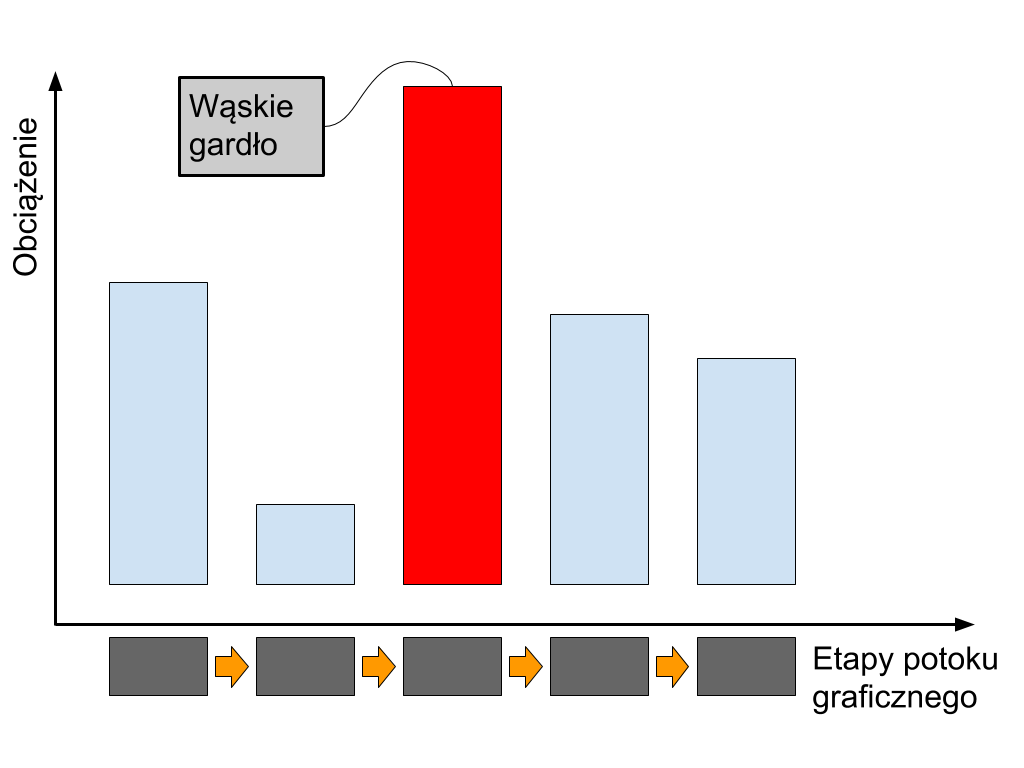
\includegraphics[width=0.4\textwidth]{res/bottleneck_locate.png}
            \caption{Lokalizacja}
            \label{fig:bottleneck_locate}
        \end{figure}
    \item Eliminacja wąskich gardeł, jeśli to możliwe (Rysunek \ref{fig:bottleneck_eliminate}) \\
        - Odciążenie etapów najbardziej obciążonych \\
        \begin{figure}[H]
            \centering
            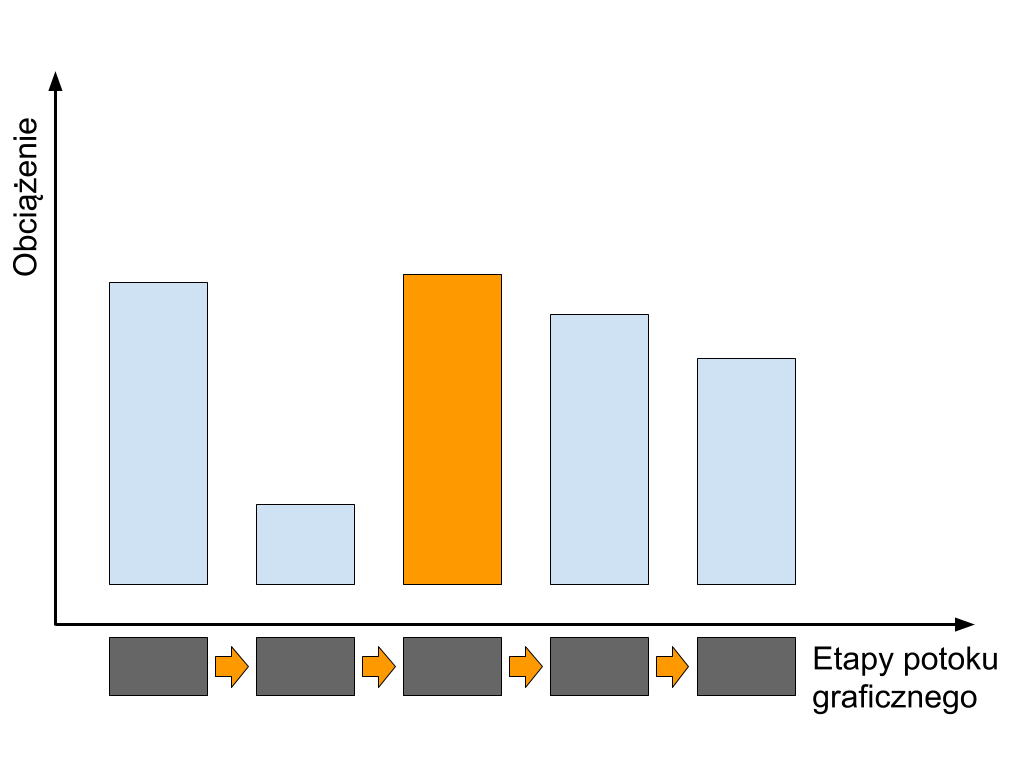
\includegraphics[width=0.4\textwidth]{res/bottleneck_eliminate.png}
            \caption{Eliminacja}
            \label{fig:bottleneck_eliminate}
        \end{figure}
    \item Zrównoważenie potoku, jeśli eliminacja wąskich gardeł niemożliwa (Rysunek \ref{fig:bottleneck_balance}) \\
        - Zwiększenie pracy innych części potoku \\
        \begin{figure}[H]
            \centering
            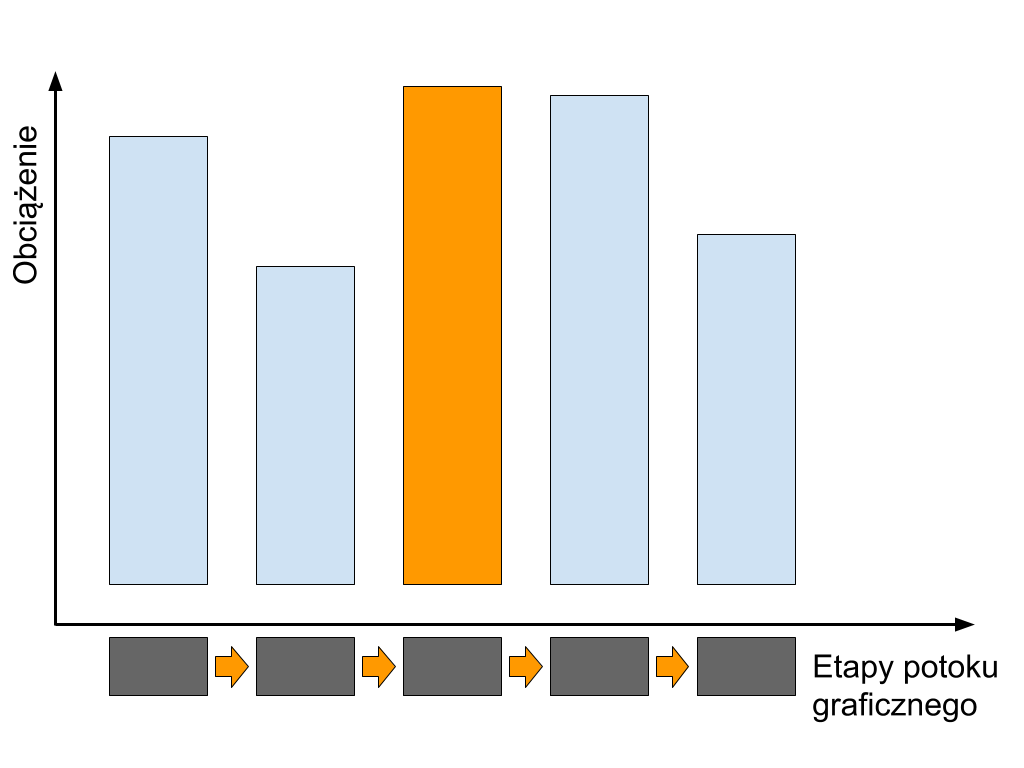
\includegraphics[width=0.4\textwidth]{res/bottleneck_balance.png}
            \caption{Zbalansowanie}
            \label{fig:bottleneck_balance}
        \end{figure}
\end{enumerate}

\section{Model potoku graficznego}
Ta praca skupia się na środowisku OpenGL, którego potok jak wielu innych systemów graficznych może zostać podzielony na trzy główne etapy (przedstawione na rysunku \ref{fig:pipeline_flow}):
\begin{itemize}
    \item Etap pracy procesora - aplikacja wykonywana przez procesor komputera, przekazuje polecania do karty graficznej.
    \item Etap geometrii - operacje wykonywane dla każdego wielokąta tworzącego model wyświetlanego obiektu. Dotyczą działań związanych z~wierzchołkami, takich jak transformacje współrzędnych, oświetlenie czy generowanie współrzędnych tekstury. \cite{bib:opengl_insights}
    \item Etap rastrowy - operacje na pikselach i~fragmentach, takie jak rysowanie wypełnionych wielokątów, mapowanie tekstur czy zapis koloru do bufora klatki.
\end{itemize}

\vbox{}

Niektóre źródła \cite{bib:top-down} wyróżniają również procesy takie jak: 
\begin{itemize}
    \item Przycinanie i~składanie prymitywów - proces transformacji pojedynczych wierzchołków w~większe struktury - prymitywy. Te elementy zostają również przycięte do okna programu wyświetlającego.
    \item Rasteryzacja - proces przejścia z~modelu opartego o~wierzchołki na obraz graficzny oparty o~piksele i~fragmenty.
\end{itemize}

\begin{figure}[H]
    \centering
    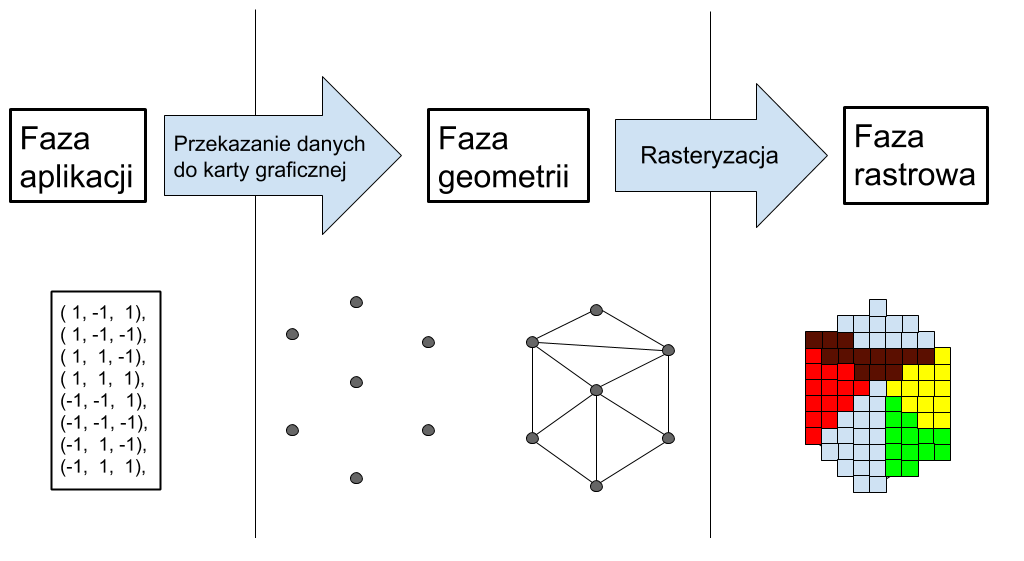
\includegraphics[width=\textwidth]{res/pipeline_flow.png}
    \caption{Fazy potoku graficznego}
    \label{fig:pipeline_flow}
\end{figure}

Pierwszym krokiem w~zwiększeniu wydajności programu jest stwierdzenie, w~którym z~etapów występuje wąskie gardło. Istnieje wiele metod sprawdzenia, który podsystem jest odpowiedzialny za spowolnienie całości systemu, na przykład, gdy podejrzewana jest faza rastrowa często wystarczy zmiana rozmiarów wyświetlacza i~sprawdzenie czy program sprawdza się lepiej. Jeżeli problem leży w~operacjach na tym poziomie system powinien mocno przyspieszyć po zmniejszeniu liczby obsługiwanych pikseli. \\
Dla każdego etapu przewidziane są również inne metody optymalizacji - jeżeli problem leży po stronie logiki aplikacji, należy przyjrzeć się fazie pracy procesora. Redukcja liczby obsługiwanych wierzchołków na pewno pomoże z~działaniami związanymi z~geometrią, a~wykorzystanie tekstur o~mniejszych rozdzielczościach odciąży podsystem rastrowy.

\section{Metody usprawnienia potoku graficznego}
Program może działać sprawniej dzięki zmianie sprzętu, na którym jest uruchamiany. Takie podejście nie jest jednak satysfakcjonujące, problem może zostać rozwiązany bez zmiany środowiska sprzętowego. Wydajność aplikacji zależy nie tylko od używanych podzespołów komputera, ale także od wielu innych czynników. Istnieje wiele technik, które umożliwiają poprawę wydajności na różnych etapach potoku graficznego. Te metody można pogrupować według ich efektów i~funkcjonalności:
\begin{itemize}
    \item Operacje przycinania danych \cite{backface_culling} \cite{game_programming_gems5} \cite{ogl_guide} - w~danej chwili wyświetlacz zazwyczaj nie pokazuje wszystkich elementów sceny trójwymiarowej. Elementy, które nie są widoczne wykorzystują cenne zasoby, nie wnosząc tym samym nic wartościowego. Techniki przycinania obiektów spoza bryły widzenia, zasłoniętych lub których powierzchnie odwrócone są w stronę środka modelu pozwalają wyeliminować tego typu składniki z~udziału w~potoku graficznym.
    \item Manipulacja poziomem szczegółów \cite{lod} \cite{lod1} \cite{lod2} \cite{lod3} \cite{lod4} \cite{bib:hoppe} - renderowanie wszystkich obiektów widocznych na ekranie w~sposób bardzo dokładny zazwyczaj ma duże konsekwencje wydajnościowe, a~niewiele korzyści jakościowych. Metody manipulacji poziomem szczegółowości zmniejszają jakość elementów mniej widocznych, oszczędzając tym zasoby na niepotrzebnie skomplikowanych modelach.
    \item Zmniejszenie obciążenia środków przesyłu danych między poszczególnymi systemami \cite{ogl_guide} \cite{bib:opengl_insights} - często to nie same procesy wykonywane na procesorze czy karcie graficznej stanowią wąskie gardło programu, ale mechanizmy transferu danych między tymi jednostkami. Techniki takie jak renderowanie instancyjne służą do zwiększania wydajności połączeń komunikacyjnych.
    \item Operacje na teksturach \cite{bib:superbible} - dwuwymiarowe grafiki można umieścić na trójwymiarowej scenie na wiele różnych sposobów, problemem zazwyczaj jest ich wielkość w~stosunku do jakości. Metody takie jak mipmapping czy filtrowanie anizotropowe pomagają zmniejszyć zasoby wymagane na poprawną obsługę tekstur.
    \item Optymalizacja pracy z~OpenGL \cite{ogl_guide} \cite{bib:superbible} - graficzny interfejs programowania aplikacji posiada wiele różnych mechanizmów, które obsłużone w~zły sposób mogą znacząco wpływać na wydajność systemu. To środowisko jest narzędziem, z~pomocą którego program ma spełniać daną funkcję. Poprawne wykorzystanie tego przyrządu jest niezbędne do uzyskania właściwych rezultatów. Mechanizmy takie jak programowalny potok graficzny i~wykorzystanie jednostek cieniujących pomagają zwiększyć wydajność programu.
    \item Czyszczenie niepotrzebnych już danych \cite{ogl_guide} \cite{bib:superbible} - informacje, które spełniły swoje zadanie i~nie są wymagane do przeprowadzenia kolejnych zadań powinny zostać zwalniane z~pamięci, robiąc tym samym miejsce dla użytecznych danych.
    \item Odciążanie głównej pętli renderującej \cite{ogl_guide} \cite{lod4} - przed rozpoczęciem wyświetlania obrazu, aplikacja może wykonać wiele czynności, których wyniki mogą zostać zapisane do późniejszego szybkiego użytku.
\end{itemize}


\section{Podstawowe zasady pomiaru wydajności}
Próba dostrojenia sprawności aplikacji opartej o~OpenGL wymaga ustalonej metryki do oszacowania wydajności programu. Testy porównawcze systemów graficznych nie różnią się niczym od weryfikowania innych operacji w~systemie komputerowym. Wśród podstawowych wskaźników wydajności wyróżnić można \cite{trapp}:
\begin{itemize}
    \item Liczba klatek na sekundę - standardowa operacja pomiaru tej wartości polega na zapisaniu wartości początkowej, wyrenderowaniu sceny i~sczytaniu wartości końcowej. Wartość porównawcza zostaje wyliczona przez podzielenie liczby wyrysowanych klatek i~upływu czasu w~sekundach. Dokładniejszy pomiar można uzyskać, na podstawie większej liczby klatek. W~celu uzyskania większej liczby danych, zaleca się zapisywanie wyników dla średniej liczby klatek na sekundę, minimalnej, maksymalnej oraz liczby pomiarów. Odwrotnością liczby klatek na sekundę jest czas trwania pojedynczej klatki, który lepiej obrazuje wzrost wydajności przy szybszym czasie wyświetlania klatki.
    \item Liczba prymitywów na sekundę - wymaga implementacji dodatkowych mechanizmów pomiarowych. Miara ta pozwala na dokładniejsze zbadanie przebiegu potoku graficznego. Dzięki tej wartości można sprawdzić jak dobrze system radzi sobie z~skomplikowanymi obiektami geometrycznymi.
    \item Liczba pikseli na sekundę - obliczanie liczby pikseli na sekundę jest nieco trudniejsze. Jednym z~prostszych sposobów jest napisanie małego programu testującego, który renderuje prymitywy o~znanym rozmiarze. Umożliwia to pomiar wydajności operacji etapu rastrowego.
\end{itemize}

\vbox{}

Pomiary powinny odbywać się w~odpowiednim środowisku testowym:
\begin{enumerate}
    \item System komputerowych nie powinien być obciążony innymi procesami niż tym, którego wydajność jest aktualnie mierzona.
    \item Pomiary powinny być prowadzone w~dostatecznie dużych odcinkach czasu (przynajmniej 100 razy większy okres niż dokładność zegara pomiarowego).
    \item Sceny testów porównawczych powinny zawierać dużą liczbę prymitywów.
    \item Zegar pomiarowy powinien zostać zatrzymany po całkowitym skończeniu pracy systemu. Niektóre operacje mogą wciąż być wykonywane w~tle, nawet po zakończonym procesie renderowania.
\end{enumerate}

\vbox{}

Poza głównymi wskaźnikami wydajności wyróżnia się dodatkowo:
\begin{itemize}
    \item Liczba prymitywów obsługiwanych w~ramach jednej klatki.
    \item Liczba obiektów obsługiwanych w~ramach jednej klatki.
    \item Liczba wierzchołków obsługiwanych w~ramach jednej klatki.
    \item Obciążenie procesora - stan wykorzystania zasobów procesora w~danej chwili.
    \item Obciążenie karty graficznej - stan wykorzystania zasobów kraty graficznej w~danej chwili.
    \item Obciążenie pamięci - zasoby pamięciowe zajmowane przez program.
\end{itemize}



\chapter{Wybrane metody poprawy wydajności[Przedmiot pracy]}

\section{Odrzucanie tylnych ścian}
Odrzucanie tylnych powierzchni (ang. \ang{Backface culling}) określa, czy dany wielokąt obiektu graficznego jest renderowany czy nie. Jest to krok w~potoku graficznym, który sprawdza czy punkty w~wielokącie pojawiają się w~kolejności zgodnej z~ruchem wskazówek zegara, czy przeciwnie do ruchu wskazówek zegara, gdy są rzutowane na ekran. Jeśli użytkownik określi, że wielokąty skierowane do przodu mają uzwojenie zgodne z~ruchem wskazówek zegara, a~wielokąt wyświetlany na ekranie ma uzwojenie przeciwne do ruchu wskazówek zegara, wówczas oznacza to, że jest on obrócony w~kierunku wnętrza bryły modelu i~nie zostanie narysowany. Oznacza to usunięcie niewidocznych trójkątów zamkniętych powierzchni przed kosztownymi operacjami rasteryzacji i~tymi wewnątrz jednostki cieniującej fragmentów.

Proces ten sprawia, że renderowanie obiektów jest szybsze i~bardziej wydajne, poprzez zmniejszenie liczby wielokątów rysowanych przez program. Generalnie nie ma potrzeby wyświetlania trójkątów tworzących powierzchnie odwrócone w~stronę wnętrza obiektu - są całkowicie zasłonięte wielokątami skierowanymi w~stronę kamery. \cite{backface_culling}

\begin{figure}[H]
    \centering
    \begin{subfigure}[b]{0.8\textwidth}
        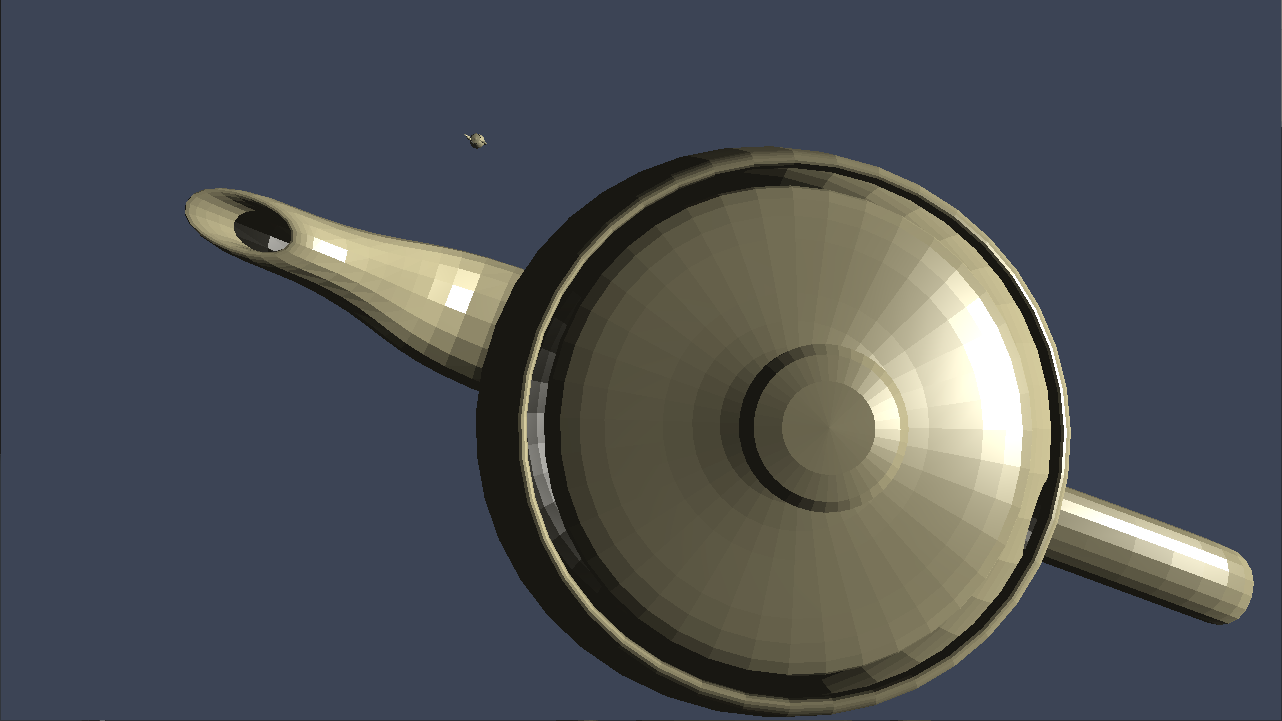
\includegraphics[width=\textwidth]{res/backface_culling_example2.png}
        \captionof{figure}{Odrzucanie tylnych ścian wyłączone}
        \label{fig:backface_culling_example2}
    \end{subfigure}
    ~ %add desired spacing between images, e. g. ~, \quad, \qquad, \hfill etc. 
    %(or a\,blank line to force the subfigure onto a\,new line)
    \begin{subfigure}[b]{0.8\textwidth}
        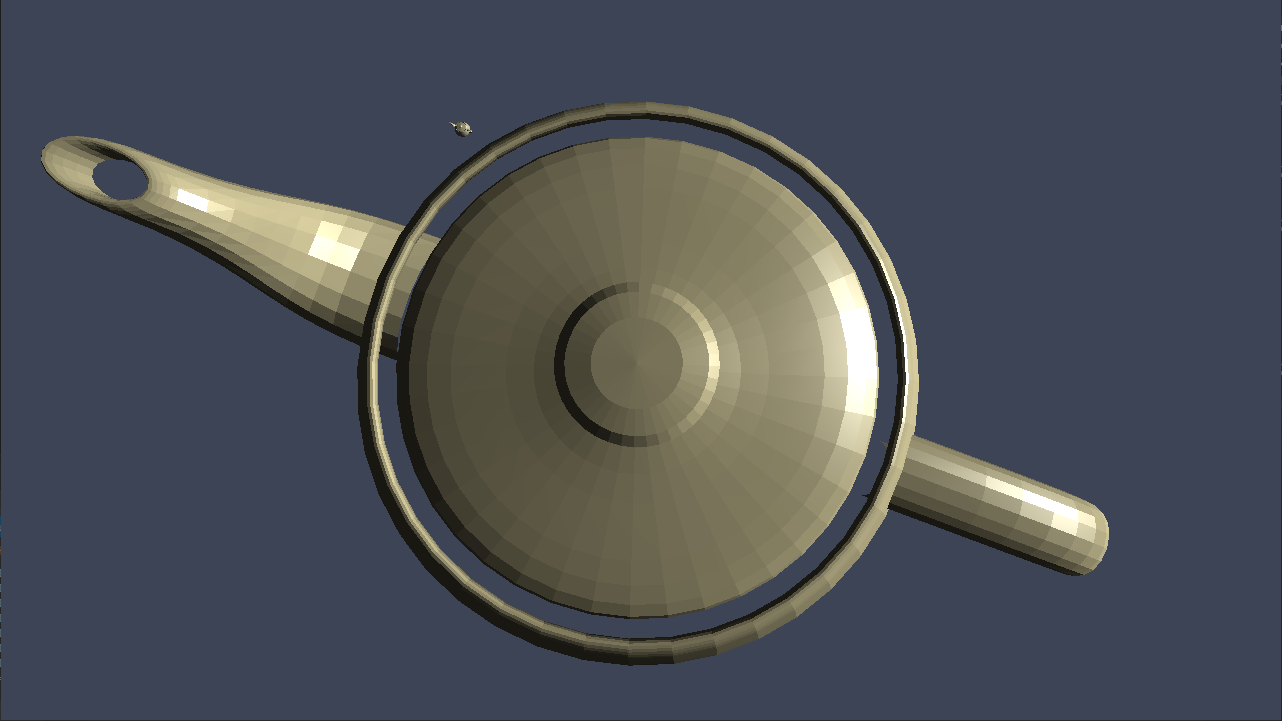
\includegraphics[width=\textwidth]{res/backface_culling_example1.png}
        \captionof{figure}{Odrzucanie tylnych ścian włączone}
        \label{fig:backface_culling_example1}
    \end{subfigure}
    \captionof{figure}{Przykład działania odrzucania tylnych ścian}
    \label{fig:backface_culling_example}
\end{figure}

Można założyć, że odrzucanie tylnej ściany nie powoduje powstania widocznych artefaktów w~renderowanej scenie, jeśli zawiera ona jedynie zamkniętą i~nieprzejrzystą geometrię. Na scenach zawierających przezroczyste wielokąty powierzchnie skierowane do wnętrza obiektu mogą stać się widoczne. Jak zostało przedstawione na rysunkach \ref{fig:backface_culling_example}, jeżeli model nie jest do końca zamknięty metoda może pozbyć się ścian które powinny zostać wyrysowane. \\
Niektóre modele umyślnie wykorzystują zestawienie powierzchni otwartych i~zamkniętych. Należy wówczas uważać, aby nie stracić informacji zawartych w~ramach obiektu.

OpenGL zapewnia wsparcie dla tej metody. Wystarczy włączyć odpowiednią opcję oraz wybrać wielokąty do wycięcia. W~tym przypadku odrzuca się oczywiście te zwrócone w~stronę wnętrza modelu.

\lstinputlisting[language=c++, caption=Aktywacja odrzucania tylnych powierzchni w~OpenGL, label=enable-backface-culling]{res/enable_backface_culling.txt}

\section{Odrzucanie obszarów spoza bryły widoku}
Kolejna metoda odrzucania elementów, których kamera nie jest w~stanie zobaczyć. Opiera się na konstrukcji bryły widoku - obszaru zawierającego wszystkie widoczne w~danej chwili obiekty. Figura jest określana na podstawie ustawień kamery i~poprzez wykorzystanie projekcji perspektywicznej przyjmuje kształt ściętej piramidy. Wszystkie obiekty znajdujące się wewnątrz zostają przekazane dalej w~potoku renderującym, pozostałe zostają odrzucone. Rysunek \ref{fig:frustrum_view} prezentuje to podejście.

\begin{figure}[H]
    \centering
    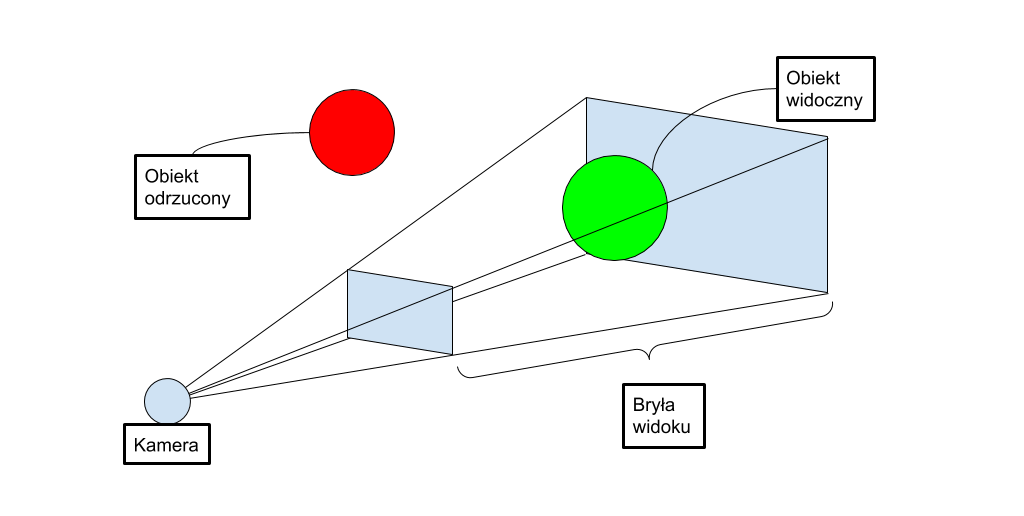
\includegraphics[width=\textwidth]{res/frustrum_view.png}
    \caption{Bryła widoku}
    \label{fig:frustrum_view}
\end{figure}

Celem tej metody jest więc identyfikacja tego, co znajduje się wewnątrz bryły widoku (całkowicie lub częściowo) i~odrzucenia wszystkiego, co nie jest w~środku. Na koniec od sprzętu graficznego wymaga się jedynie renderowania tego, co jest widoczne, co pozwala zaoszczędzić na przetwarzaniu wszystkich tych wierzchołków, które i~tak nie są dostrzegalne. Oznacza to odciążenie sprzętu i~zazwyczaj poprawia wydajność programu.

Ta metoda ma sens, jeśli część sceny, która znajduje się w~bryle widoku, jest znacznie mniejsza niż sama scena. W~skrajnym przypadku, gdy cały świat trójwymiarowy jest zawsze widoczny, odrzucanie obszarów spoza bryły widzenia to strata czasu, ponieważ nie ma nic do wycięcia. Taka sytuacja nie zdarza się jednak często, a~potencjalne korzyści w~zakresie wydajności mogą być bardzo znaczące.

Istnieje wiele różnych wersji tej techniki, a~większość z~nich sprowadzają się do dwóch etapów: konstrukcji bryły widoku i~sprawdzenia czy obiekt się w~niej znajduje.

\subsection{Podejście geometryczne}
To podejście samo w~sobie zawiera wiele wariacji, przedstawiona tu wersja przedstawia każdą płaszczyznę tworzącą bryłę widoku jako punkt do niej należący oraz jej wektor normalny, skierowany do środka figury. W~celu wyznaczenia tych danych potrzebne są następujące parametry:
\begin{itemize}
    \item pozycja i~rotacja kamery,
    \item kąt pola widzenia,
    \item odległości dalekiej i~bliskiej płaszczyzny od kamery,
    \item stosunek szerokości do wysokości ekranu.
\end{itemize}
Rysunek \ref{fig:frustrum_geo_params} obrazuje te parametry w~odniesieniu do kamery i~jej pola widzenia.

\begin{figure}[H]
    \centering
    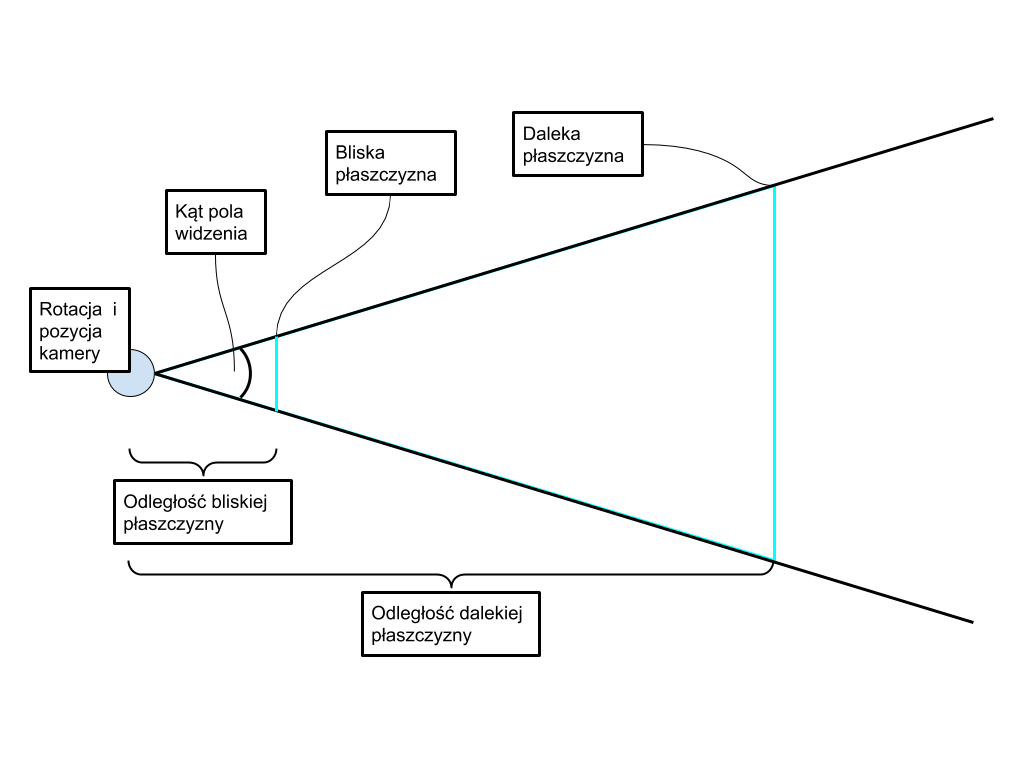
\includegraphics[width=\textwidth]{res/frustrum_geo_params.png}
    \caption{Parametry potrzebne do wyznaczenia płaszczyzn określających bryłę widoku}
    \label{fig:frustrum_geo_params}
\end{figure}

Kiedy wyznaczone zostały już płaszczyzny określające bryłę widoku można przejść do sprawdzenia które obiekty znajdują się w~jej środku. W~tym celu wyliczana zostaje odległość obiektu od każdej z~powierzchni. Ze względu na wektor normalny płaszczyzny ujemny wynik przy co najmniej jednym sprawdzeniu oznacza, że element leży poza bryłą widoku. \\
Pozostaje tylko wyznaczyć punkt, na podstawie którego ma być wyliczana ta odległość. Najprościej obliczyć tą wartość dla każdego wierzchołka modelu i~jeżeli chociaż jeden z~nich leży wewnątrz bryły widoku cały obiekt powinien zostać wyrenderowany. Takie podejście wiąże się jednak z~duża ilością obliczeń i~sporym obciążeniem wydajności.  \\
Rozwiązaniem tego problemu może być konstrukcja bryły ograniczającej dla każdego obiektu. Ten twór za pomocą prostej reprezentacji ma opisywać obszar zawierający wszystkie wierzchołki modelu. Wówczas zamiast każdego z~wierzchołków obiektu sprawdzona zostanie tylko utworzona struktura. Oczywiście wiąże się to z~pewną niedokładnością, mimo to warto jednak skorzystać z~takiego podejścia. Proces ten zostanie opisany na przykładzie sfery. \\
Sfera ograniczająca dany obiekt przedstawia jest jako punkt, będący jej środkiem oraz jej promień. Te dane obliczane są przez wyznaczenie średniej pozycji wszystkich wierzchołków modelu, a~następnie zmierzenie odległości między tym punktem, a~najbardziej oddalonym od niego wierzchołkiem. Odległości od każdej z~płaszczyzn określających bryłę widoku obliczana jest względem środka sfery. Jeżeli ta wartość dla co najmniej jednej z~powierzchni jest mniejsza od ujemnej wartości promienia to obiekt zostaje odrzucony - znajduje się poza bryłą widoku.

\lstinputlisting[language=c++, caption=Sprawdzenie czy sfera ograniczające znajduje się wewnątrz bryły widoku, label=frustrum-geo-check]{res/frustrum_geo_check.txt}

W kolejnych metodach omówione zostanie tylko przycinanie punktu, podejście do sfery ograniczającej jest analogiczne do tego powyżej.

\subsection{Podejście przestrzeni przycinającej}
Ta metoda sprowadza się do zaprojektowania macierzy, przekształcającej punkty do przestrzeni przycinającej. W~tym wymiarze bryła widoku jest sześcianem o~środku w~punkcie (0, 0, 0) i~boku o~długości równiej 2. Tworzące ją powierzchnie zdefiniowane są poprzez punkty:
\begin{itemize}
    \item powierzchnia górna: (0, 1, 0),
    \item powierzchnia dolna: (0, -1, 0),
    \item powierzchnia prawa: (1, 0, 0),
    \item powierzchnia lewa: (-1, 0, 0),
    \item powierzchnia przednia: (0, 0, 1),
    \item powierzchnia tylna: (0, 0, -1).
\end{itemize}
Po przekształceniu punktu do tej przestrzeni sprawdzenie czy leży on w~środku bryły przycinającej staje się bardzo proste. Zakładając, że ten przerobiony punkt to $p = (x, y, z)$, wystarczy sprawdzić:\\
\begin{align}
-1 < &x < 1 \\
-1 < &y < 1 \\
-1 < &z < 1
\end{align}
Jeżeli te warunki pozostają spełnione punkt znajduje się wewnątrz bryły widoku, w~przeciwnym wypadku zostaje odrzucony. Trudnością w~tym podejściu jest przekształcenie danych do przestrzeni przycinającej lub wyznaczenie równań na płaszczyzny ograniczające bryłę widoku w~tej przestrzeni.

\subsection{Podejście radarowe}
Ta metoda różni się od pozostałych tym, że nie konstruuje się tutaj bezpośrednio bryły widoku, a~raczej bada położenie danego punktu. Na początku jednak należy przekształcić współrzędne elementów sceny do układu współrzędnych opartego o~kamerę. Taki układ zakłada, że położenie kamery to zawsze punkt (0, 0, 0) oś X zwrócona jest bezpośrednio w~prawą stronę kamery, oś Y w~górę, a~oś Z~w przód (odwrotnie niż w~OpenGL). \cite{game_programming_gems5} Rysunek \ref{fig:frustrum_radio_ref} obrazuje taki system. \\
Przekształcenie punktu $p$ do takiego układu współrzędnych odbywa się za pomocą prostej operacji - od jego współrzędnych zostają odjęte wartości współrzędnych kamery $cc$. Punkt wynikowy oznaczony jako $pc$.

\begin{align}
pc &= p - cc \\
\Rightarrow pc.z &= p.z - cc.z \\
\Rightarrow pc.y &= p.y - cc.y \\
\Rightarrow pc.x &= p.x - cc.x
\end{align}

\begin{figure}[H]
    \centering
    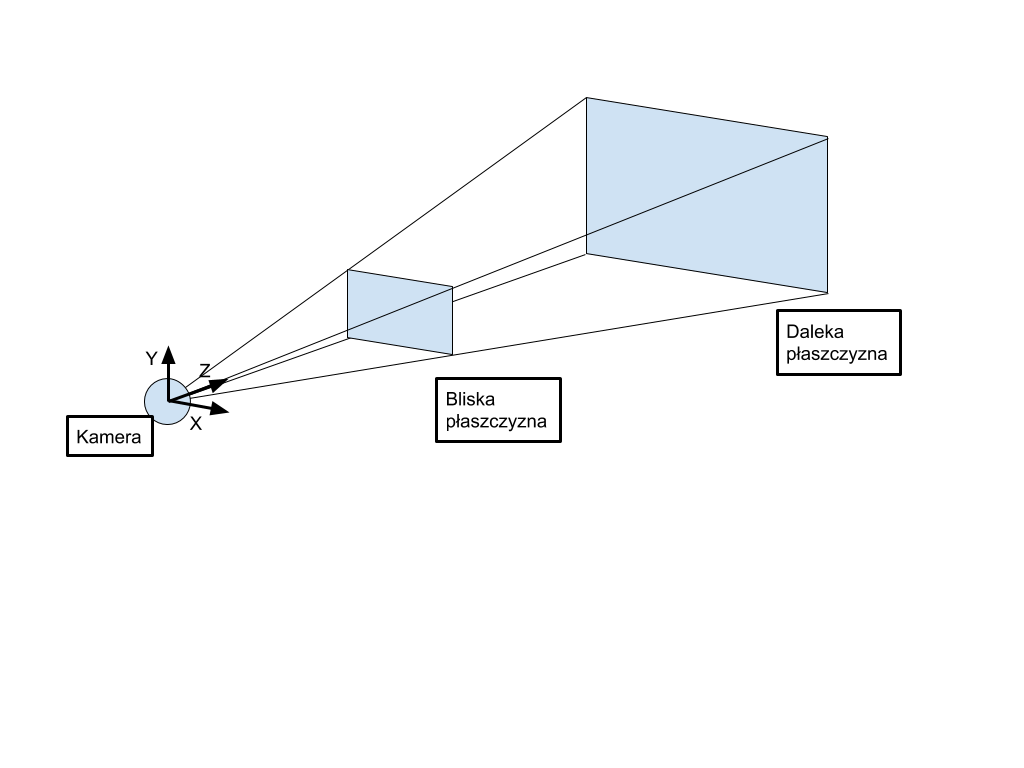
\includegraphics[width=0.9\textwidth]{res/frustrum_radio_ref.png}
    \caption{Układ współrzędnych kamery}
    \label{fig:frustrum_radio_ref}
\end{figure}

Kiedy współrzędne badanego punktu zapisane zostały w~układzie współrzędnych kamery można przystąpić do analizy jego położenie. Wymagane wartości do przeprowadzenie tej operacji obejmują:
\begin{itemize}
    \item kąt pola widzenia,
    \item odległości dalekiej i~bliskiej płaszczyzny od kamery,
    \item stosunek szerokości do wysokości ekranu.
\end{itemize}
Kolejno analizowane zostają pojedyncze współrzędne punktu. Składowa Z~jest porównywana z~odległościami dalekiej ($dp$) i~bliskiej ($bp$) płaszczyzny od kamery, jeżeli badana wartość znajduje się pomiędzy nimi punkt nie zostaje odrzucony.
\begin{equation}
    bp < pc.z < dp
\end{equation}

Współrzędna X i~Y badane są podobnie, najpierw należy wyznaczyć wartość $h$ i~$w$ - wysokość i~szerokość bryły widoku dla współrzędnej Z~punktu. Wykorzystany zostanie tu kąt pola widzenia $a$ oraz stosunek szerokości do wysokości ekranu $r$. Rozmieszczenie parametrów zostało zilustrowanie na rysunku \ref{fig:frustrum_radio_h}.

\begin{figure}[H]
    \centering
    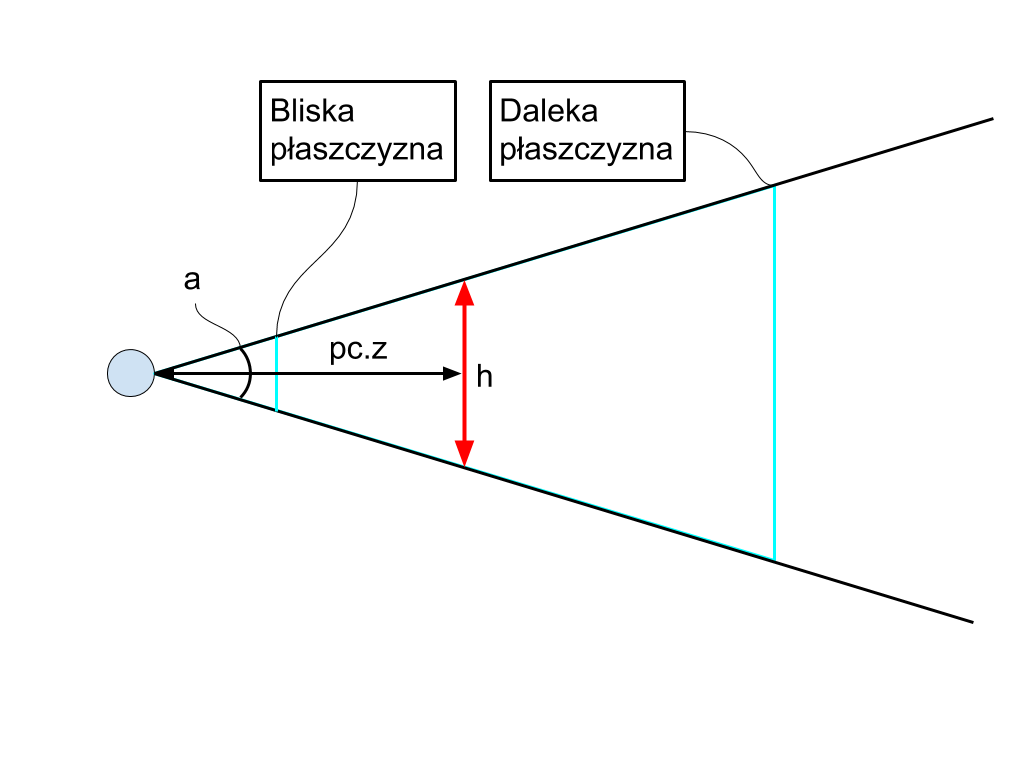
\includegraphics[width=0.5\textwidth]{res/frustrum_radio_h.png}
    \caption{Obliczanie wysokości bryły widoku dla współrzędnej Z~punktu}
    \label{fig:frustrum_radio_h}
\end{figure}

\begin{align}
h &= pc.z * 2 * tg(a/2) \\
w &= h * r
\end{align}

Wykorzystując te wartości można określić czy współrzędne X i~Y punktu znajdują się wewnątrz bryły widoku.
\begin{align}
-h/2 < &pc.y < h/2 \\
-w/2 < &pc.x < w/2
\end{align}
Jeżeli wszystkie współrzędne punktu spełniają nałożone ograniczenia punkt leży wewnątrz bryły widzenia i~może zostać wyrenderowany.

\vbox{}

\textbf{W pracy wykorzystane zostało podejście geometryczne.} Jest to metoda klasyczna i~najlepiej oddająca sposób działania tej techniki. Na potrzeby testów i~pracy zostało przyjęte to rozwiązanie, ponieważ stanowi ono podstawę, na której pozostałe zostały oparte.

\section{Poziom szczegółowości}
Manipulacja poziomem szczegółów (ang. \ang{Level of Detail}) – zmniejszenie złożoności modelu obiektu w~zależności od odległości od kamery. Zazwyczaj tę technikę stosuje się tylko do detali geometrii, jednak koncepcja może zostać uogólniona na wiele różnych aspektów. Na przykład przy zarządzaniu jednostkami cieniującymi, w~celu zachowania kontroli nad złożonością pikseli. W~tej pracy technika zajmuje się redukcją liczby wierzchołków modelu, co pozwala na zwiększenie efektywności renderowania poprzez zmniejszenie obciążenia na niektórych etapach potoku graficznego, zwykle tych zajmujących się transformacjami wierzchołków. Rysunek \ref{fig:lod_example} przedstawia model na kilku poziomach szczegółowości. \\
Wyróżniono dwa podstawowe podejścia do tego zagadnienia. \cite{lod}

\begin{figure}[H]
    \centering
    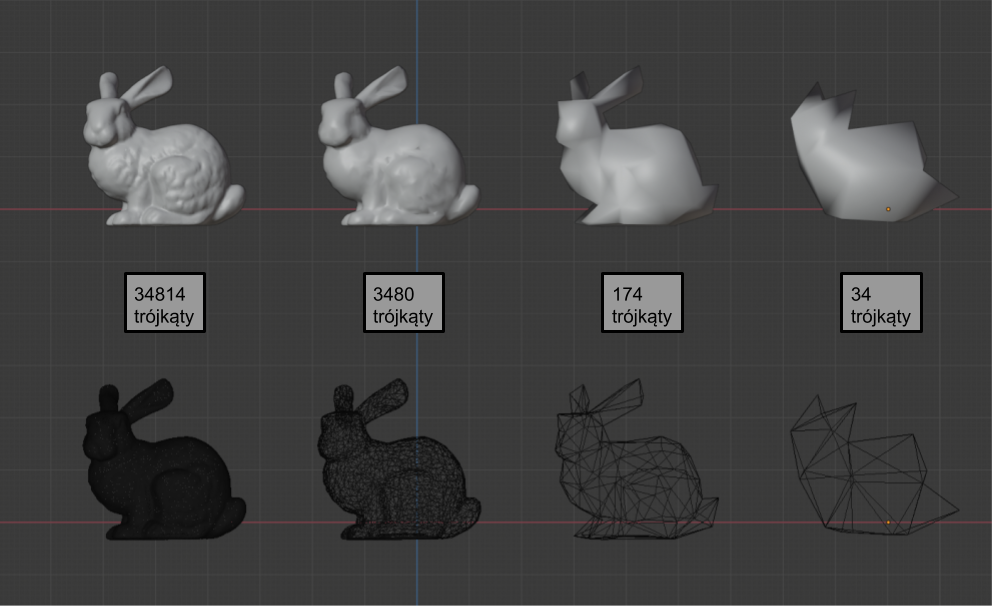
\includegraphics[width=\textwidth]{res/lod_example.png}
    \caption{Przykład kolejnych poziomów szczegółów}
    \label{fig:lod_example}
\end{figure}

\subsection{Podejście dyskretne}
Polega na tworzeniu wielu dyskretnych wersji oryginalnej geometrii ze zmniejszonymi poziomami szczegółów geometrycznych. W~czasie pracy programu modele z~pełnymi szczegółami są zastępowane wariantami o~zmniejszonej szczegółowości lub na odwrót, w~zależności od pozycji kamery. Zdefiniowane zostają zakresy odległości, w~ramach których wykorzystywane są różne stopnie detali. Niektóre warianty tej metody zakładają całkowite usunięcie obiektu z~potoku graficznego, jeżeli znajduje się on w~odpowiedniej pozycji. Ze względu na dyskretną naturę poziomów zamiana jednego modelu na inny może być widoczna. \cite{lod4} \cite{lod} \\
Rysunek \ref{fig:lod_discrete_ranges} obrazuje strefy poszczególnych poziomów szczegółów.

\begin{figure}[H]
    \centering
    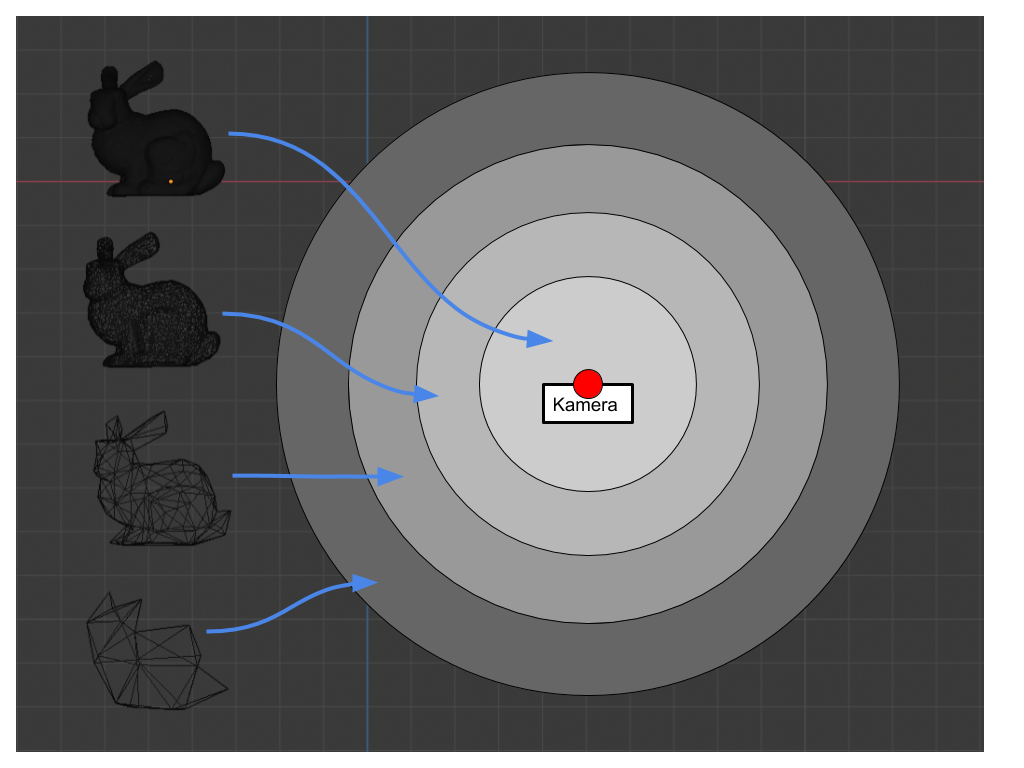
\includegraphics[width=\textwidth]{res/lod_discrete_ranges.png}
    \caption{Zakresy poziomów szczegółowości}
    \label{fig:lod_discrete_ranges}
\end{figure}

\subsection{Podejście ciągłe}
Zamiast dyskretnych zakresów odległości od kamery ta metoda stosuje stale zmienne spektrum szczegółów geometrycznych. Zazwyczaj dany tutaj jest tylko jeden model o~najwyższym poziomie detali oraz algorytm lub heurystyka, która w~trakcie działania programu przycina liczbę wierzchołków w~zależności od parametru decydującego. Podejście to wymaga ciągłego wykonywania potrzebnych obliczeń w~trakcie pętli renderującej, co może znacząco wpłynąć na wydajność pracy programu. Zalety tej metody obejmują rozwiązanie problemu z~przejściami między dyskretnymi wariantami modelu oraz wsparcie dla bardzo dużych obiektów. Przy dostatecznie dużych rozmiarach jeden koniec elementu może znajdować się bardzo blisko kamery, a~drugi daleko, dobranie odpowiedniego poziomu detali może w~takiej sytuacji okazać się problematyczne. Technika ciągła pozwala na wykorzystanie różnych poziomów szczegółowości dla poszczególnych obszarów obiektu. \cite{lod} \cite{bib:hoppe}

\textbf{W pracy wykorzystane zostało podejście dyskretne.} Zapewnia dużą wydajność, modele w~kolejnych zakresach poziomów szczegółów konstruowane są jeszcze przed rozpoczęciem pętli renderującej. Przy wyświetlaniu elementów sprawdzana jest jedynie odległość od kamery i~na jej podstawie wstawiana jest odpowiednia wersja modelu. Wersje o~zmniejszonej szczegółowości zostały tak przygotowane (redukcja nie jest gwałtowna), że efekt wizualny związany z~zamianą jednego modelu na drugi jest prawie niewidoczny. Obiekty nie są na tyle duże, żeby wymagany był różny poziom szczegółowości w~jednym obszarze i~inny w~drugim. 

\lstinputlisting[language=c++, caption=Wybór modelu poziomu szczegółów w~pętli renderującej, label=lod-render]{res/lod_render.txt}

W ramach sceny można wyróżnić dwie główne grupy obiektów, na których zastosowanie metody manipulacji poziomem detali może okazać się bardzo skuteczne. Ze względy na różnice w~strukturze tych elementów można na nich zastosować różne techniki generowania poziomów detali. Grupy składników, o~których mowa to:
\begin{itemize}
    \item Obiekty - istnieje wiele różnych technik generowania rzetelnych wersji modeli o~zmniejszonym poziomie szczegółowości, na przykład Algorytm Rozpadu Krawędzi (ang. \ang{Edge Collapse}) \cite{lod2} \cite{lod} lub Połowiczny Algorytm Rozpadu Krawędzi (ang. \ang{Half-Edge Collapse}) \cite{lod1}.
    \item Teren - zastosowane może tutaj zostać nieco inne podejście, siatka terenu zazwyczaj jest bardzo regularna i~prosta w~porównaniu do obiektów. Dzięki temu prostsze algorytmy, takie jak Geometryczny Mipmapping (ang. \ang{Geometrical Mipmapping}) \cite{lod3}, mogą zostać wykorzystane. Na rysunku \ref{fig:lod_terrain_example} został przedstawiony przykład z~działania metody manipulacji poziomem szczegółów terenu zastosowanej w~niniejszej pracy.
    \begin{figure}[H]
        \centering
        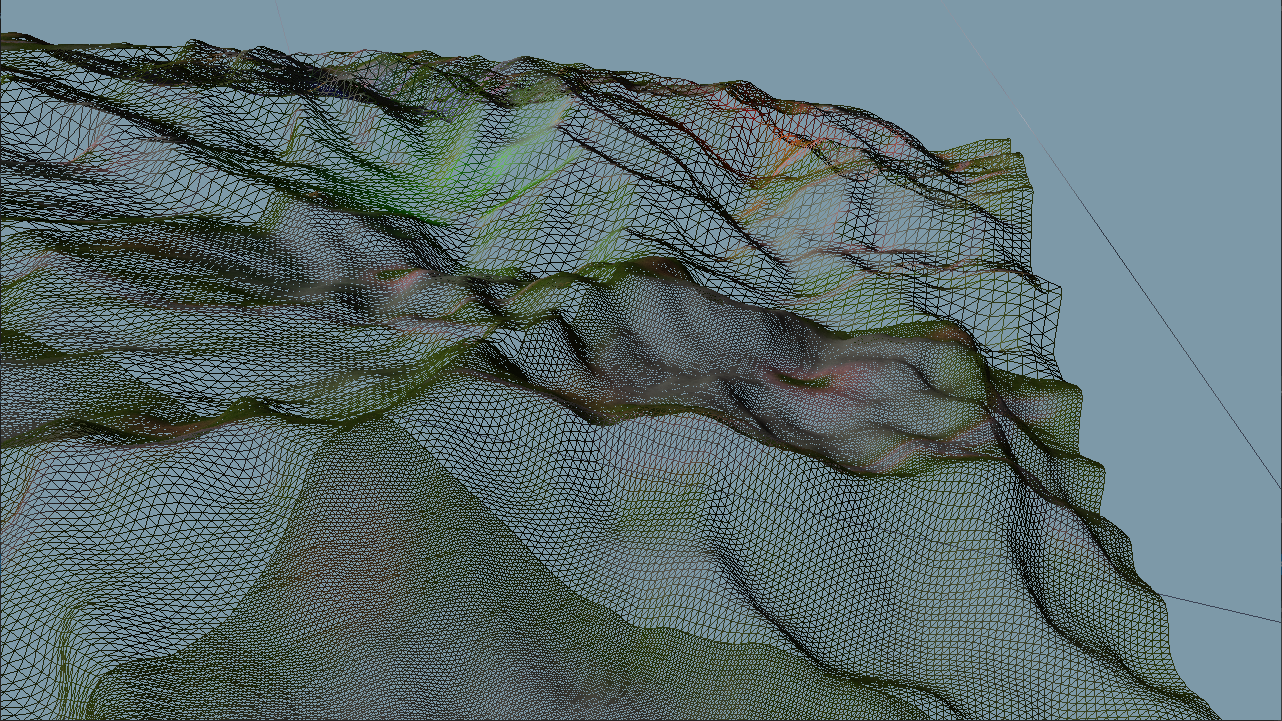
\includegraphics[width=0.9\textwidth]{res/lod_terrain_example.png}
        \caption{Przykład manipulacji poziomem szczegółów terenu}
        \label{fig:lod_terrain_example}
    \end{figure}
\end{itemize}

\section{Renderowanie instancyjne}
Przy rysowaniu wielu instancji tego samego modelu wąskim gardłem, negatywnie wpływającym na wydajność, może okazać się liczba odwołań renderujących. Dużo zasobów zużytych zostaje na samą komunikację między procesorem a~kartą graficzną. Przy każdym odwołaniu OpenGL musi wykonać niezbędne przygotowania, zanim będzie mógł przekazać dane wierzchołków. Więc nawet jeśli renderowanie wierzchołków jest bardzo szybkie, przekazywanie poleceń ich renderowania takie nie jest. Poszczególne instancje jednego modelu zazwyczaj różnią się tylko niewielką liczbą parametrów, takich jak rozmieszczenie na scenie, skala czy obrót. \cite{bib:opengl_insights} \\
Renderowanie instancyjne pozwala na renderowanie wielu instancji tego samego obiektu przy pomocy tylko jednego odwołania do karty graficznej. Rysunki \ref{fig:instancing_chart1} i~\ref{fig:instancing_chart2} obrazują to podejście. W~OpenGL dostępne są różne mechanizmy pozwalające jednostkom cieniującym używać instancji odwołania rysowania jako danych wejściowych i~wykorzystywać różne wartości atrybutów wierzchołków na instancję, a~nie na wierzchołek. \cite{ogl_guide}

\begin{figure}[H]
    \centering
    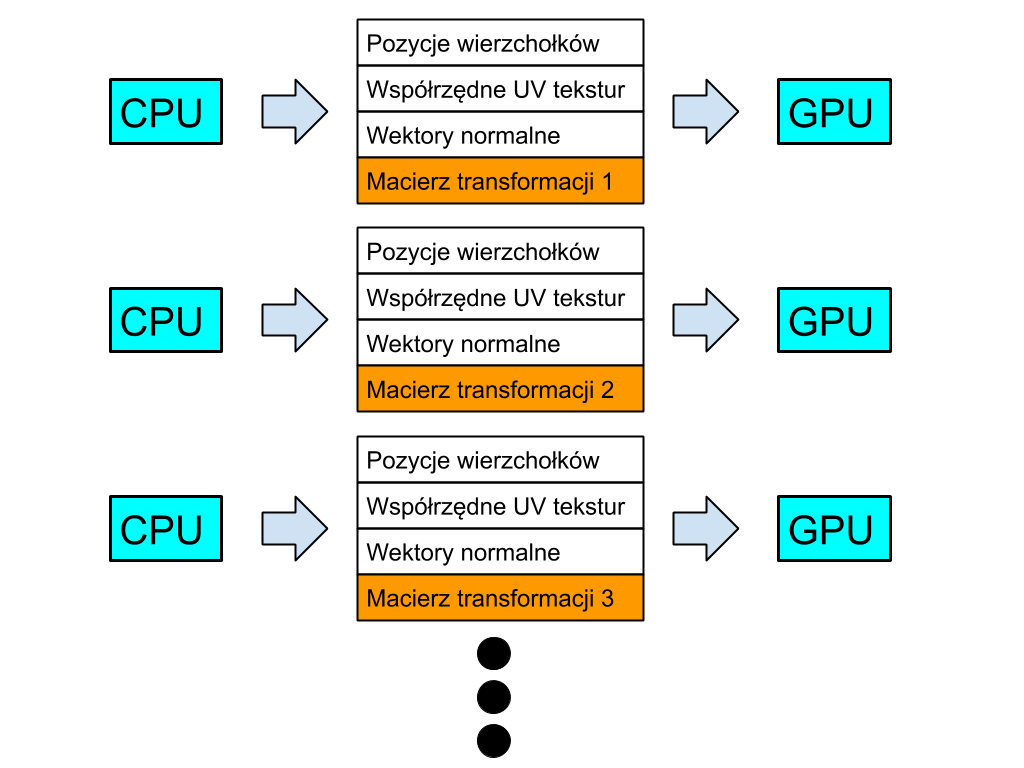
\includegraphics[width=0.8\textwidth]{res/instancing_chart1.png}
    \caption{Bez instancjonowania}
    \label{fig:instancing_chart1}
\end{figure}
~ %add desired spacing between images, e. g. ~, \quad, \qquad, \hfill etc. 
%(or a\,blank line to force the subfigure onto a\,new line)
\begin{figure}[H]
    \centering
    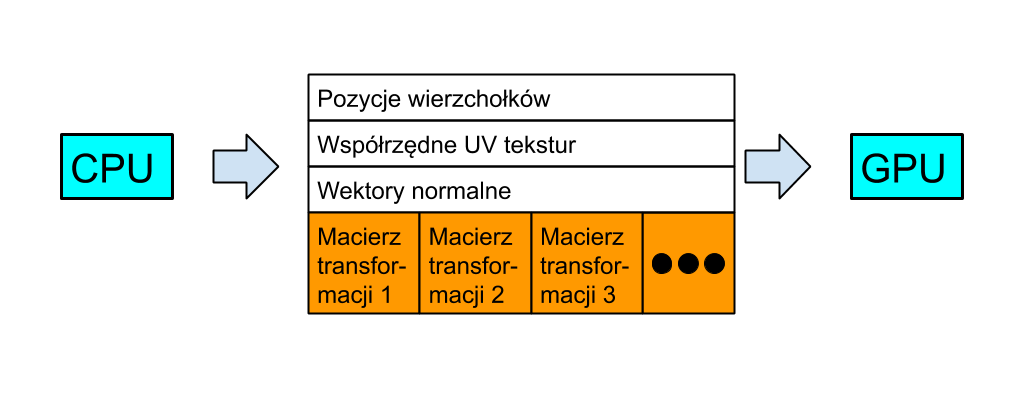
\includegraphics[width=0.8\textwidth]{res/instancing_chart2.png}
    \caption{Renderowanie instancyjne}
    \label{fig:instancing_chart2}
\end{figure}

W jednostkach cieniujących każda instancja posiada własny identyfikator dostępny przez zmienną środowiskową \texttt{gl\_InstanceID}. W~pracy nie została ona jednak wykorzystana, zamiast tego użyto tablic instancyjnych. Definiowane jako parametry wejściowe jednostki cieniującej, pozwalają na przechowywanie i~przenoszenie znacznie większej ilości danych. W~kodzie programu, przed przesłaniem informacji, należy oznaczyć dane jako instancyjne oraz ustawić, które wartości mają zostać przyporządkowane do której instancji.

\section{Mipmapping}
Metoda poprawy jakości wyświetlania tekstur - generuje i~wykorzystuje wiele wersji grafiki o~niższych rozdzielczościach przy renderowaniu obszarów, które zajmują mniej pikseli na ekranie niż oryginalna tekstura. Generalnie zastosowanie tej metody sprowadza się do dwóch przypadków:
\begin{itemize}
    \item oteksturowana powierzchnia znajduje się daleko od kamery,
    \item element jest widoczny pod pewnym kątem.
\end{itemize}
Mipmapping pozwala na wykorzystanie grafik niższej rozdzielczości, co korzystnie wpływa na wydajność silnika i~nie oddziałuje negatywnie lub nawet poprawia jakość obrazu wynikowego.

\begin{figure}[H]
    \centering
    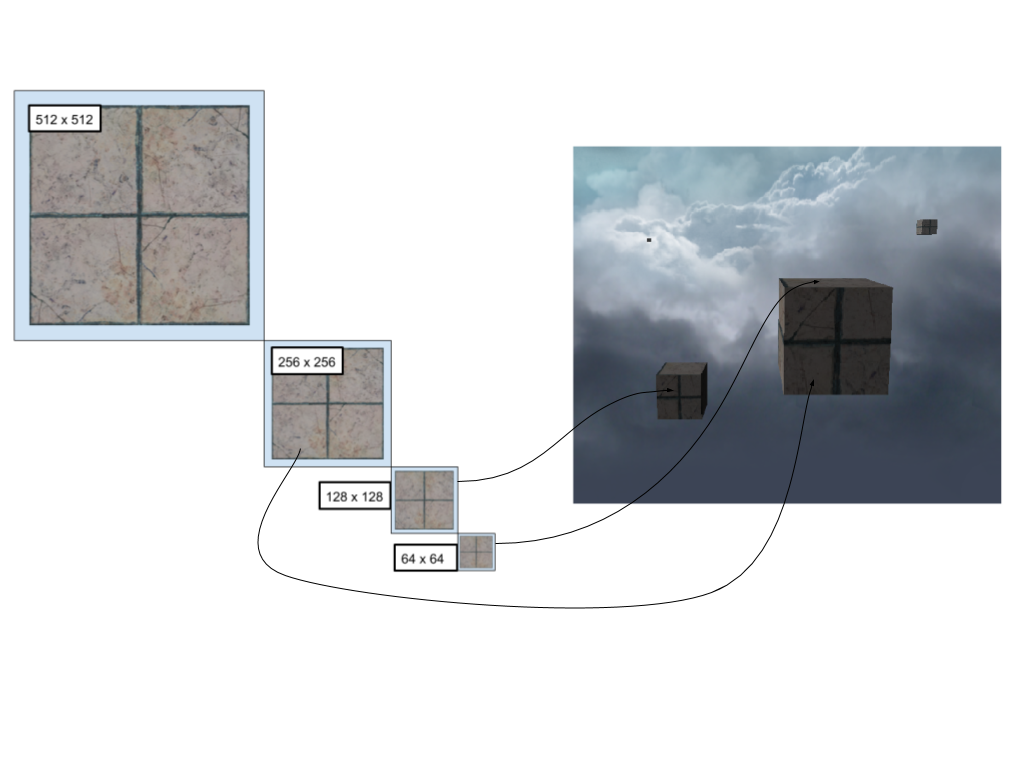
\includegraphics[width=\textwidth]{res/mipmapping_textures.png}
    \caption{Mipmapping - wersje tekstury}
    \label{fig:mipmapping_textures}
\end{figure}

Technika bardzo dobrze radzi sobie z~powierzchniami zwróconymi bezpośrednio przodem do kamery, jednak pod dużym kątem zauważyć można jej wady. Tekstura, przez swój stały format, nie dopasowuje się dobrze, gdy obszar zmienia swoje wymiary. Jak przedstawiono na rysunku \ref{fig:mipmapping_textures} niektóre powierzchnie widziane pod kątem wykorzystują niskie rozdzielczości tekstur, co jest poprawne dla jednego z~wymiarów, jednak dla drugiego grafika jest rozciągnięta.

\subsection{Filtrowanie anizotropowe}
Filtrowanie anizotropowe to rozszerzenie mipmappingu. Stosuje nie tylko liniowo zmniejszone wersje tekstur, ale również grafiki o~innych wymiarach niż pierwotna wersja obrazu. Dzięki temu dla obszarów widzianych pod kątem możliwe staje się lepsze dopasowanie tekstur. Przykład obrazujący to podejście został przedstawiony na rysunku \ref{fig:anisotropy_textures}.

\begin{figure}[H]
    \centering
    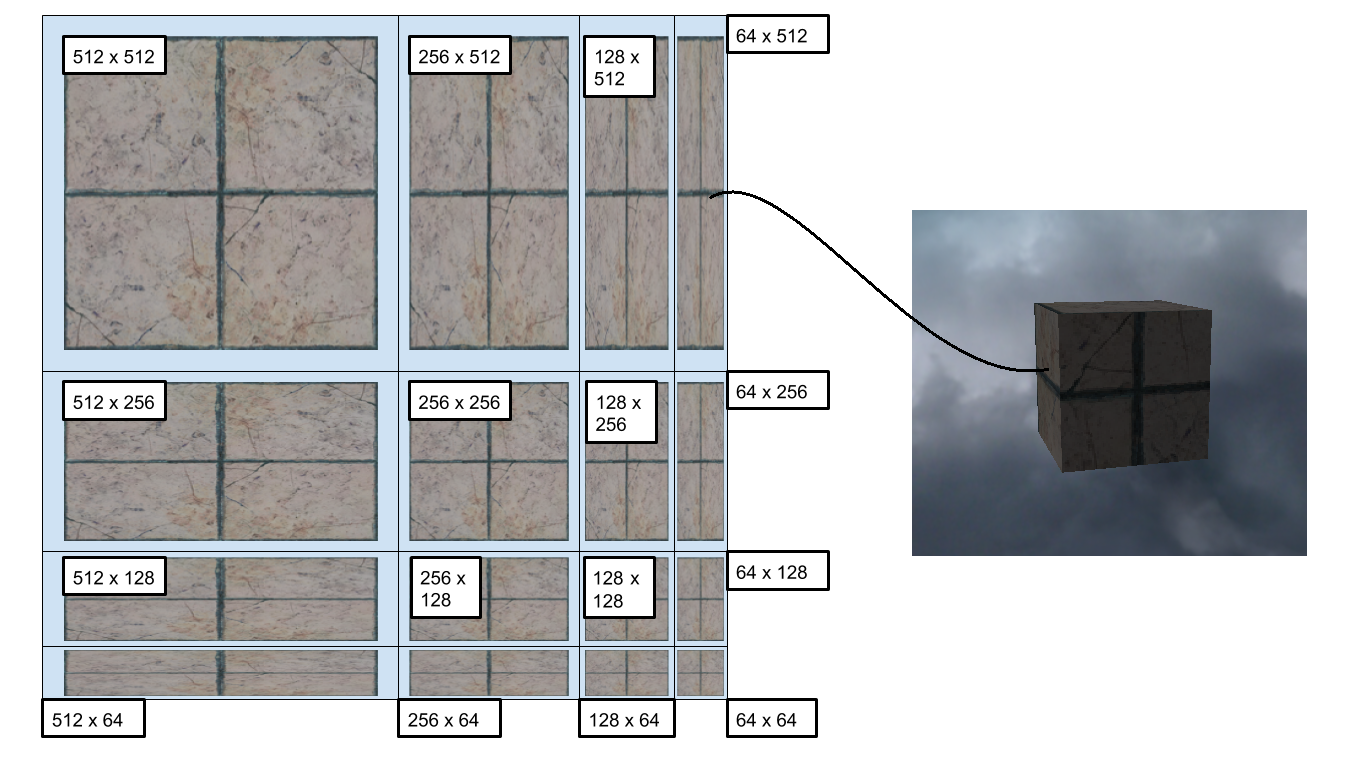
\includegraphics[width=\textwidth]{res/anisotropy_textures.png}
    \caption{Filtrowanie anizotropowe - wersje tekstury}
    \label{fig:anisotropy_textures}
\end{figure}

Zarówno mipmapping jaki i~filtrowanie anizotropowe pomagają pozbyć się szumu który występuje na rozległych powierzchniach opatrzonych w~tekstury o~dużych rozdzielczościach. Przez wykorzystanie tekstur o~mniejszych wymiarach obydwie techniki mogą pozytywnie wpłynąć na wydajność programu, zwłaszcza mipmapping. Jeżeli chodzi o~filtrowanie anizotropowe to metoda ta jest raczej używana w~celu poprawy jakości obrazu końcowego, niż do zwiększenia wydajności. Tekstury wyjściowe posiadają większą rozdzielczość niż w~przypadku mipmappingu, a~odpowiednia ich generacja i~obsługa wymaga wykorzystania dużych zasobów systemu, które zazwyczaj są zbyt kosztowne dla potencjalnych korzyści wydajnościowych. Parametrem filtrowania anizotropowego jest stopnień próbkowania, decyduje o~jakości filtrowania, przy wyższych wartościach tej zmiennej wydajność zazwyczaj jest odczuwalnie niższa. \cite{bib:superbible} \\

OpenGL zapewnia wsparcie zarówno dla mipmappingu, jaki i~filtrowania anizotropowego. Przy wczytywaniu tekstury należy ustawić odpowiednie flagi, aktywujące wewnętrzną implementacje OpenGL oraz dostosować parametry pracy obydwu metod. Im wyższa wartość tym lepszy efekt, ale również bardziej kosztowny wydajnościowo. Nie wszystkie systemy i~wersje środowiska OpenGL wspierają omawiane metody - przed ich obsługą należy sprawdzić stanowisko pracy. \\

W pracy wykorzystane zostały obie techniki, przy czym badania zajmują się głównie mipmappingiem ze względu na jego wpływ na wydajność.


\chapter{Badania}

\section{Metodyka badań}
W celu przeprowadzenia badań zaprojektowana i~zaimplementowana została aplikacja badawcza. Program sprawdza się jako silnik graficzny oparty o~OpenGL i~to na jego podstawie przeprowadzone zostały testy. Aplikacja w~wersji podstawowej nie używa żadnej z~badanych metod poprawy wydajności i~stanowi podstawę do analizy porównawczej. Względem wartości, zmierzonych w~tym wariancie programu, został sprawdzony wpływ poszczególnych metod poprawy wydajności. \\
Aplikacja jest zdolna do wyrenderowania scen, zawierających różne elementy grafiki trójwymiarowej i~wykorzystujących wiele efektów i~mechanizmów, używanych w~profesjonalnych programach graficznych. Przewidzianych zostało wiele wariantów scenerii testowych, sprawdzających aspekty pracy różnych etapów potoku renderowania. \\
Wszystkie testy odbywały się w~tym samym środowisku sprzętowym przy zbliżonym obciążeniu komputera na tej samej wersji programu (z niektórymi funkcjonalnościami wyłączonymi dla poszczególnych testów porównawczych). \\
Narzędzia zewnętrzne zostały wykorzystane do zebrania potrzebnych wartości, na podstawie których przeprowadzona została analiza. Część danych była sczytywana bezpośrednio z~interfejsu aplikacji lub zapisywana do plików w~trakcie przebiegu testu. \\

\vbox{}

Testy zostały podzielone na dwie grupy, w~ramach których pomiary przebiegały w~inny sposób.
\begin{itemize}
    \item Testy statyczne - pozycja kamery i~jej obrót są stałe. Obraz nie zmienia się poza elementami sceny poruszającymi się samodzielnie. Takie podejście pozwala na zbadanie pracy programu dla stosunkowo niezmiennego otoczenia. Niektóre metody poprawy wydajności nie są zależne od pozycji kamery, więc jej zmiana w~czasie nie wniosłaby nic nowego. W~tych testach mierzone jest obciążenie systemu, które w~innych eksperymentach jest mniej stabilne i~trudniejsze do odczytu.
    \item Testy dynamiczne - zaprojektowany został zestaw ruchów kamery po scenie, który jest dokładnie powtarzany w~każdym teście. Zmiany pozycji i~rotacji zdefiniowane są dla każdej klatki trwania pętli renderującej, są niezależne od prędkości działania aplikacji. Na każdy eksperyment składa się 7200 klatek. Kamera przemieszcza się bo całej powierzchni sceny, dochodzi do miejsc, gdzie obiekty występują gęściej lub rzadziej, zbliża i~oddala się od pojedynczych elementów oraz obraca w~górę, w~dół i~na boki.
\end{itemize}
W ramach tych grup inne wartości wskaźników wydajności zostały zbierane (sekcja \ref{section:benchamarks}).\\
Testy przebiegały w~następujący sposób: na początku dla każdego wariantu przewidzianego dla badanej metody zmierzone i~zapisane zostały wartości wskaźników wydajności z~wersji bazowej aplikacji. Następnie kolejno angażowane były badane metody. Pierwszy test każdej metody zawsze odbywa się w~standardowym wariancie sceny 1 w~trybie statycznym. Sprawdzony został stan programu z~każdą metodą działającą osobno oraz z~kombinacją wszystkich mechanizmów. Wyniki zostały zebrane i~przedstawione w~tabelach w~sekcji \ref{section:wyniki}.

\section{Podstawowe środowisko badawcze}
Aplikacja badawcza ma za zadanie skonstruowanie środowiska umożliwiającego przeprowadzenie testów. W~ramach pracy zaimplementowana zastała wersja podstawowa narzędzia, umożliwiająca między innymi wyświetlenie scen, na których przeprowadzone zostały testy. Aplikacja bazowa nie posiada żadnych z~opisywanych metod poprawy wydajności, stanowi ona punkt odniesienia, względem którego odbywały się testy i~do którego zostały porównane wyniki. \\

Wersja podstawowa została następnie rozbudowana o~techniki poprawy wydajności, które zostały przebadane. Na potrzeby testów metody były kolejno włączane i~wyłączane, skonstruowany został również prosty interfejs konsolowy pozwalający na wybór sceny. \\

Silnik został zbudowany od podstaw w~celu kontroli funkcjonalności i~pracy programu. Aplikacja opiera się o~niskopoziomowy interfejs programowania aplikacji OpenGL oraz kilka bibliotek pomocniczych. Mechanizmy i~narzędzia potrzebne do prawidłowego wyświetlenia i~konstrukcji scen zostały napisane od podstaw. Dzięki temu, możliwe było wprowadzenie modyfikacji i~usprawnień na niskim poziomie. Na rynku istnieje wiele gotowych rozwiązań, które bez wątpienia lepiej radzą sobie z~renderowaniem obrazów, jednak dokładny wgląd i~zmiany w~podstawach ich działania jest utrudniony, przez co praca badawcza może być trudna.

\subsection{Dane techniczne}
Aplikacja została napisana w~języku \texttt{C++} w~środowisku Microsoft Visual Studio 2017 Enterprise. 

Silnik graficzny wykorzystuje następujące narzędzia:
\begin{itemize}
    \item OpenGL (ang. \ang{Open Graphics Library} - Otwarta Biblioteka Graficzna) - programistyczny interfejs aplikacji grafiki 2D i~3D. Jest niezależny od systemu okien i~systemu operacyjnego. OpenGL umożliwia programistom oprogramowania tworzenie wydajnych, atrakcyjnych wizualnie aplikacji graficznych na komputery PC, stacje robocze i~sprzęt superkomputerowy na rynkach takich jak projektowanie komputerowe, rozrywka, tworzenie gier, produkcja, medycyna i~wirtualna rzeczywistość. OpenGL pozwala na pracę ze wszystkimi funkcjami najnowszego sprzętu graficznego. Interfejs programowania aplikacji jest zdefiniowany jako zestaw funkcji, które mogą być wywoływane przez program użytkownika wraz z~zestawem wartości stałych.
    
    Narzędzie wykorzystuje język GLSL (ang. \ang{OpenGL Shading Language} - Język Cieniowania OpenGL) do pracy z~jednostkami cieniującymi. Jego składnia zbliżona jest do języka \texttt{C} i~jest bezpośrednio wspierany przez interfejs OpenGL. \\
    Wykorzystana wersja OpenGL: 4.3.0 \\
    Wykorzystana wersja GLSL: 430
    \item GLFW (ang. \ang{Graphics Library Framework} - Środowisko OpenGL) - wielopratformowa i~otwartoźródłowa biblioteka napisana w~języku \texttt{C} stworzona do pracy z~OpenGL. Pozwala na tworzenie i~pracę z oknami, kontekstami OpenGL oraz obsługę urządzeń wejściowych takich jak klawiatura, mysz czy manipulator drążkowy. \\
    Wykorzystana wersja GLFW: 3.3.2
    \item GLEW (ang. \ang{Graphics Library Extension Wrangler} - Treser Rozszerzeń OpenGL) - wieloplatformowa, otwartoźródłowa biblioteka, służąca do wczytywania rozszerzeń \texttt{C/C++}. GLEW zapewnia wydajne mechanizmy uruchomieniowe do określania, które rozszerzenia OpenGL są obsługiwane na platformie docelowej. Rdzeń i~funkcje OpenGL są widoczne w~jednym pliku nagłówkowym. GLEW został przetestowany na różnych systemach operacyjnych. \\
    Wykorzystana wersja GLEW: 2.1.0
    \item GLM (ang. \ang{Graphics Library Mathematics} - Matematyka OpenGL) - matematyczna biblioteka \texttt{C++}, zawierająca tylko nagłówki. Jest przeznaczona dla aplikacji graficznych i~oparata jest o~specyfikacje GLSL. Zapewnia wiele funkcjonalności takich jak: transformacje macierzy, kwaterniony, pakowanie danych, liczby losowe, szum i~inne.\\
    Wykorzystana wersja GLM: 0.9.9.3
    \item stb - niewielka biblioteka domeny publicznej dla języków \texttt{C/C++} wspomagająca pracę z~obrazami. Składa się na nią wiele samowystarczalnych, pojedynczych plików. W~tej pracy wykorzystywany jest konkretnie pakiet \texttt{stb\_image.h} do obsługi grafik w~formacie \texttt{.png}.
\end{itemize}

\subsection{Opis funkcjonalności}
Zadaniem silnika renderującego jest wyświetlanie grafiki trójwymiarowej na ekranie komputera, może wykorzystać do tego kilka metod (na przykład śledzenie promieni (ang. \ang{Ray-tracing})). Większość takich programów wykorzystuje właśnie interfejsy programowania aplikacji takie jak OpenGL, Direct3D czy Vulkan, zamiast bezpośredniej pracy z~kartą graficzną i~procesorem komputera. Silniki graficzne zazwyczaj są później wykorzystywane przez inne aplikacje. \\
Aplikacja badawcza używana w~ramach tej pracy posiada wiele mechanizmów umożliwiających zbudowanie i~wyświetlenie sceny trójwymiarowej na ekranie.

\subsubsection{Obsługa modeli w~formacie \texttt{.obj}}
Aplikacja badawcza do poprawnego wyrenderowania obiektu potrzebuje następujących elementów:
\begin{itemize}
    \item trójwymiarowych pozycji wierzchołków,
    \item zmapowanych współrzędnych tekstur,
    \item wektorów normalnych,
    \item indeksów powyższych składników, składających się na każdy trójkąt.
\end{itemize}
Format zapisu informacji o~trójwymiarowym modelu \texttt{.obj} zawiera wszystkie te informacje, ale do poprawnej obsługi plików konieczna była implementacja mechanizmu wczytującego i~interpretującego pobrane dane. \\ Przykład pliku został przedstawiony poniżej na listingu \ref{obj-example}.

\lstinputlisting[language=c++, caption=Przykładowy plik \texttt{.obj}, label=obj-example]{res/obj_example.txt}

Struktura pliku \texttt{.obj} przedstawia się następująco:
\begin{itemize}
    \item Nagłówek - zawiera informacje o~pliku i~o środowisku, w~jakim został utworzony.
    \item Linie rozpoczynające się od znaku 'o' - nazwa obiektu składowego modelu, informacja nie jest wykorzystywana w~pracy.
    \item Linie rozpoczynające się od znaku 'v' - trójwymiarowy wektor, którego składniki odpowiadają współrzędnym wierzchołka modelu.
    \item Linie rozpoczynające się od znaków 'vt' - wektor dwuwymiarowy, zawierający dane o~zmapowanych współrzędnych tekstury.
    \item Linie rozpoczynające się od znaków 'vn' - trójwymiarowy wektor normalny wierzchołków.
    \item Linie rozpoczynające się od znaku 'f' - reprezentują trójkąty modelu oraz odpowiadające im wektory współrzędnych wierzchołków, tekstur oraz normalne. Informacje zapisane są w~formacie a/b/c d/e/f g/h/i, wszystkie wartości a, b, c, d, e, f, g, h, i~są liczbami naturalnymi. Każdy z~tych trzech członów zawiera informacje, gdzie można znaleźć dane dotyczące jednego z~wierzchołków trójkąta. \\
    Liczby a, d, g to indeksy linii zawierających dane o~współrzędnych wierzchołka. \\
    Liczby b, e, h to indeksy linii zawierających dane o~współrzędnych tekstur. \\
    Liczby c, f, i~to indeksy linii zawierających dane o~wektorach normalnych.
\end{itemize}
Należy dodać, że indeksy poszczególnych elementów nie odpowiadają sobie, to znaczy, że jeden wierzchołek może posiadać wektor normalny o~danym indeksie i~wektor współrzędnych o~zupełnie innym indeksie. Dlatego ostatni element (poprzedzony znakiem 'f') jest bardzo ważny przy składaniu modelu w~jedną całość. \\
W programie wszystkie elementy zostają posortowane według ostatniego składnika i~zapisane w~tablicach. Następnie te tablice zostają przekształcone na obiekty VBO \footnote{VBO (ang. \ang{Vertex Buffer Object}) - 
Obiekt Bufora Wierzchołków - struktura interfejsu OpenGL umożliwiająca wczytanie i~pracę z~wartościami wektorowymi. 
Jest wykorzystywany jako źródło danych tablicy wierzchołków.} i~wczytane do VAO \footnote{VAO (ang. \ang{Vertex Array Object}) - 
Obiekt Tablicy Wierzchołków - struktura interfejsu OpenGL przechowująca format danych wierzchołków oraz obiekty VBO, zapewniające tablice danych wierzchołków.}, gdzie są gotowe do użycia przez OpenGL. \\
Modele \texttt{.obj} wykonane na potrzeby pracy zostały opracowane z~pomocą darmowego programu Blender 2.80.

\subsubsection{Obsługa tekstur w~formacie \texttt{.bmp} i~\texttt{.png}}
Tekstury wykorzystywane w~aplikacji badawczej początkowo zapisywane były w~formacie \texttt{.bmp}, jednak ze względu na duży rozmiar zaimplementowana została również obsługa grafik \texttt{.png}. Do wczytania i~dekodowania z~pliku i~pamięci wykorzystana została publiczna biblioteka \texttt{stb}. \\

\begin{figure}[H]
    \centering
    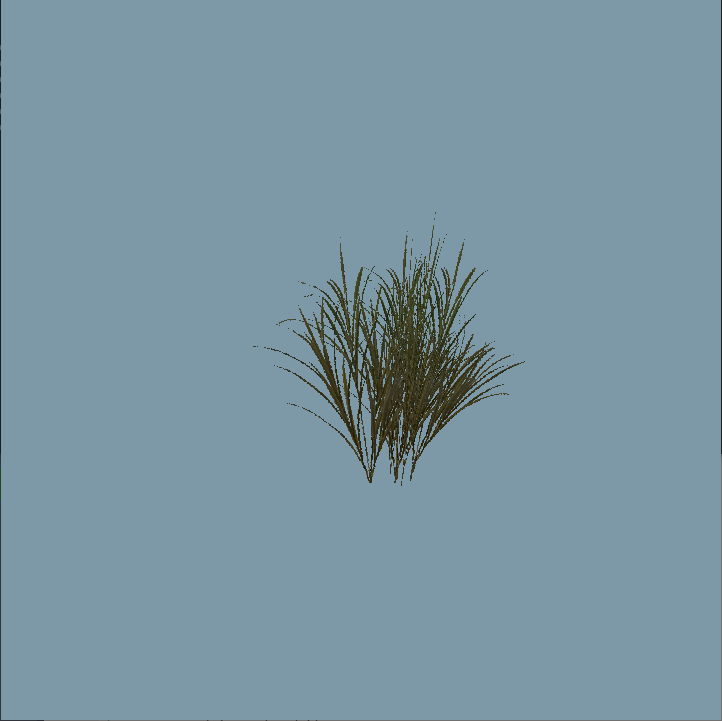
\includegraphics[width=0.5\textwidth]{res/transparency_example.png}
    \caption{Przykład przeźroczystej tekstury}
    \label{fig:transparency_example}
\end{figure}

Wykorzystanie formatu \texttt{.png} pozwala również na użycie kanału alfa do uzyskania przeźroczystych części obiektu (rysunek \ref{fig:transparency_example}). Realizacja tego mechanizmu odbywa się w~jednostce cieniującej fragmentów. Fragmenty posiadające wartość kanału alfa mniejszą od zadanej stałej zostają odrzucone (listing \ref{transparency-frag}).

\lstinputlisting[language=c++, caption=Jednostka cieniująca fragmentów - przeźroczystość, label=transparency-frag]{res/transparency_frag.txt}

\subsubsection{Model oświetlenia}
Model oświetlenia odpowiada za stwierdzenie która część sceny jest widoczna i~w~jakim stopniu. Obiekty posiadają swoje własne tekstury, które definiują jego kolor w~danym pikselu, jednak to od oświetlenia zależy z~jaką intensywnością widoczny jest ten piksel. Kolor światła również ma znaczenie, jest on mieszany z~kolorem danego elementu sceny i~określa odcień odblasku. \\
Na tym etapie źródło światła zostało zdefiniowane poprzez jego pozycję i~kolor. \\
Oświetlenie sceny składa się z~trzech składników:
\begin{itemize}
    \item Światło rozproszone - poziom oświetlenia tym światłem zależy od tego, jak bardzo dana powierzchnia zwrócona jest w~stronę źródła światła (Rysunek \ref{fig:diffuse}). W~celu obliczenia tej wartości wykorzystane zostały normalne wierzchołków zapisane w~pliku \texttt{.obj}. Przy przekazaniu danych z~jednostki cieniującej wierzchołków do jednostki cieniującej fragmentów wartości normalnych są interpolowane po całej powierzchni prymitywu. \par
    \begin{figure}[H]
        \centering
        \begin{subfigure}[b]{0.4\textwidth}
            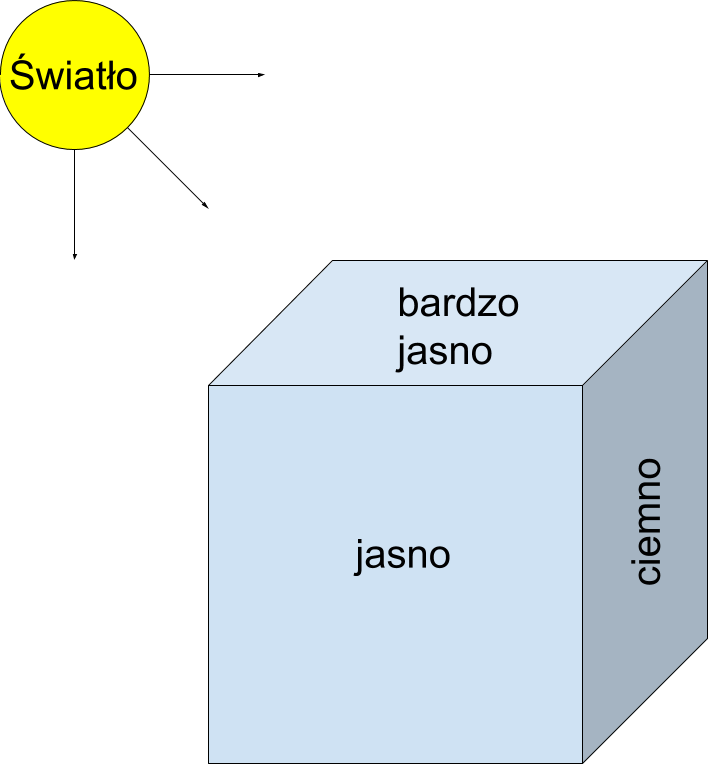
\includegraphics[width=\textwidth]{res/diffuse_brightness.png}
            \captionof{figure}{Wizualizacja oświetlenia obiektu}
            \label{fig:diffuse_brightness}
        \end{subfigure}
        ~ %add desired spacing between images, e. g. ~, \quad, \qquad, \hfill etc. 
        %(or a\,blank line to force the subfigure onto a\,new line)
        \begin{subfigure}[b]{0.5\textwidth}
            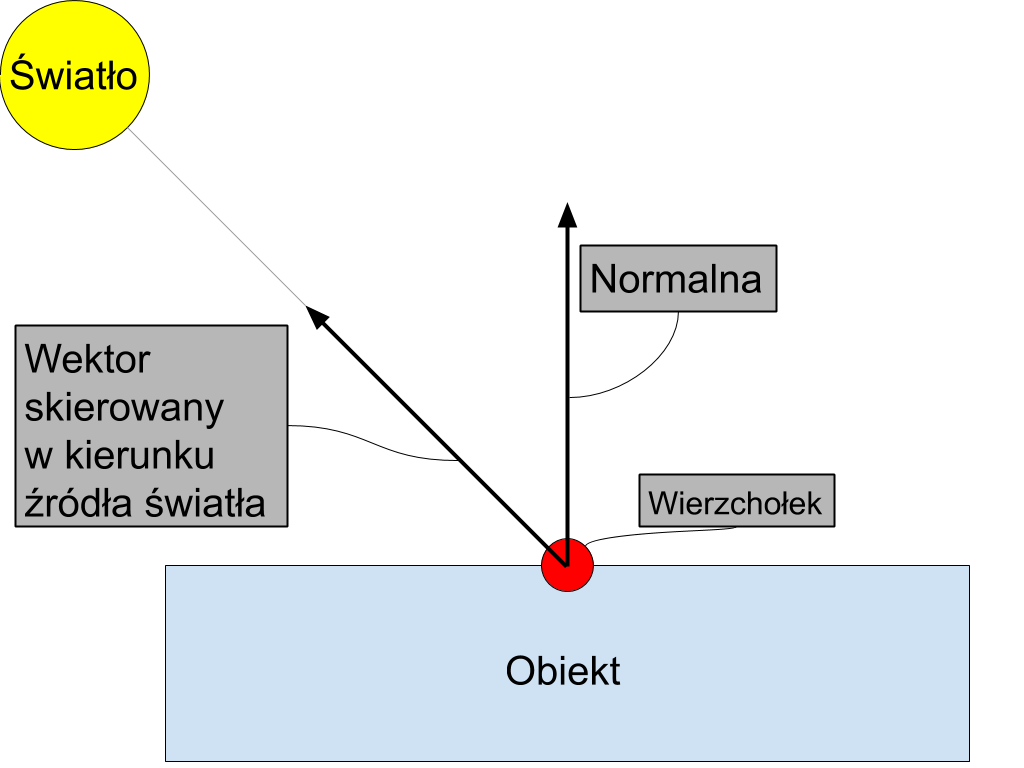
\includegraphics[width=\textwidth]{res/diffuse_vectors.png}
            \captionof{figure}{Wektory potrzebne do wyliczenia współczynnika rozproszenia}
            \label{fig:diffuse_vectors}
        \end{subfigure}
        \captionof{figure}{Zależność nasycenia światła i~obrotu względem źródła światła}
        \label{fig:diffuse}
    \end{figure}
    Jak widać na rysunku \ref{fig:diffuse}b stopień nachylenia powierzchni w~stronę źródła światła można zdefiniować za pomocą iloczynu skalarnego dwóch wektorów:
    \begin{itemize}
        \item wektora normalnego w~danym punkcie,
        \item wektora zwróconego z~danego punktu w~stronę źródła światła.
    \end{itemize}
    Ujemne wartości iloczynu skalarnego zostają zmienione na 0. Otrzymaną w~ten sposób liczbę z~zakresu [0, 1] pozostaje już tylko przemnożyć przez kolor tekstury w~danym punkcie. Większość procesu odbywa się w~jednostce cieniującej fragmentów, której uproszczony do opisanego stanu kod został przedstawiony na listingu \ref{diffuse-frag}.
    
    \lstinputlisting[language=c++, caption=Jednostka cieniująca światła rozproszonego, label=diffuse-frag]{res/diffuse_frag.txt}
    
    \item Światło zwierciadlane - światło odbite od powierzchni obiektu. Nie zastępuje światła rozproszonego, ale jest na nie nakładane. Generalnie dzięki dodaniu tego elementu uzyskany zostaje efekt odblasku.
    \begin{figure}[H]
        \centering
        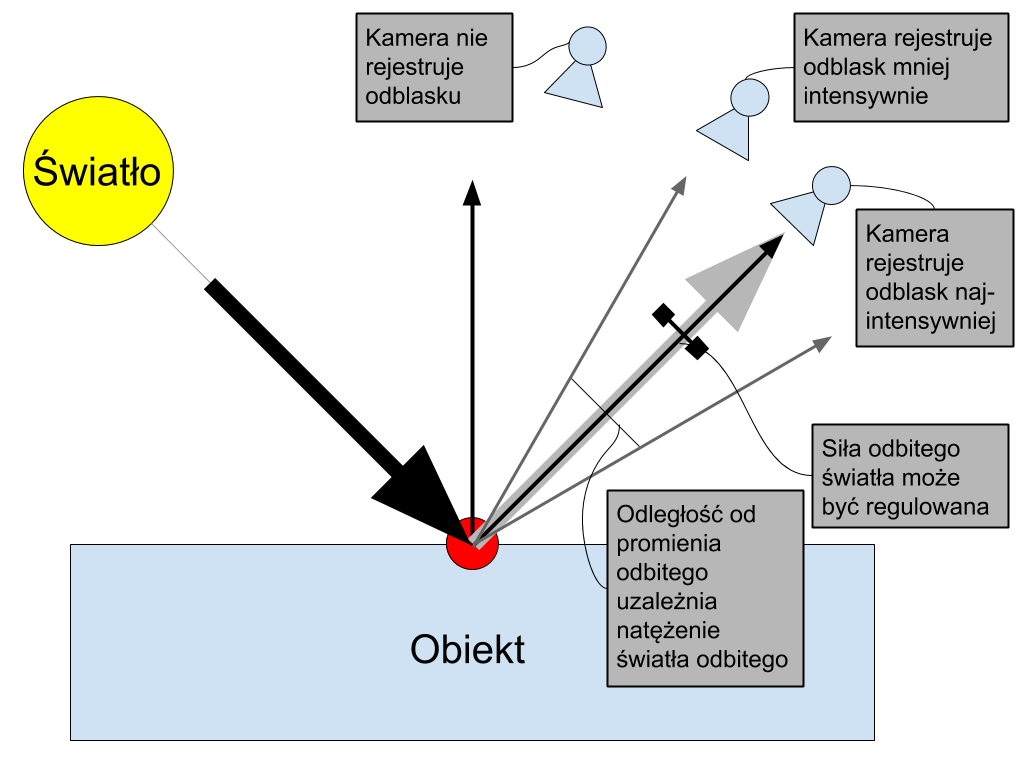
\includegraphics[width=\textwidth]{res/specular_vectors.png}
        \caption{Czynniki wpływające na światło zwierciadlane}
        \label{fig:specular_vectors}
    \end{figure}
    
    Natężenie, zasięg oraz intensywność tego światła zależy od kilku czynników (rysunek \ref{fig:specular_vectors}):
    \begin{itemize}
        \item Położenie źródła światła względem normalnej danego punktu - kąt odbicia jest równy kątowi padania, przy czym oba są liczone od normalnej punktu. 
        \item Zmienna odpowiedzialna za siłę odblasku - światło może zostać całkowicie odbite lub z~pewną stratą, wartość tej straty jest ustawiana za pomocą zmiennej.
        \item Położenie kamery - odblask jest oczywiście widoczny, gdy promień odbity wpada bezpośrednio w~kamerę, ale jest on również widzialny, gdy kamera znajduje się w~pobliżu tego promienia. Im położenie kamery jest bliższe temu stojącemu bezpośrednio na drodze promienia odbitego, tym odbłysk jest bardziej intensywny.
        \item Zmienna tłumienia połysku - to jak daleko kamera może oddalić się od bezpośredniego promienia odbitego i~dalej rejestrować odblask jest ustawiane przy pomocy kolejnej zmiennej.
    \end{itemize}
    
    Do wyliczenia światła zwierciadlanego koniecznym było wyznaczenie dodatkowych wektorów:
    \begin{itemize}
        \item wektora od źródła światła do punktu,
        \item wektora promienia odbitego,
        \item wektora od punktu do kamery.
    \end{itemize}
    Następnie na podstawie zmiennej tłumienia połysku iloczynu skalarnego wektora promienia odbitego oraz wektora od punktu do kamery wyliczony zostaje współczynnik tłumienia. \\
    Wzór na wartość światła zwierciadlanego w~danym punkcie przedstawia się następująco:
    \begin{equation}
        \vec{l} = max(\vec{r} \bullet \vec{c}, 0)^{D} * R * \vec{k}
    \end{equation}
    gdzie:
    \begin{itemize}
        \item $\vec{l}$ - wartość światła zwierciadlanego w~danym punkcie,
        \item $\vec{r}$ - wektor promienia odbitego,
        \item $\vec{c}$ - wektor od punktu do kamery,
        \item D - zmienna tłumienia połysku,
        \item R - zmienna siły odblasku,
        \item $\vec{k}$ - kolor światła,
        \item $\bullet$ - iloczyn skalarny.
    \end{itemize}
    
    Poniżej przedstawiony został kod jednostki cieniującej fragmenty poszerzony o~wyliczenia światła zwierciadlanego dla jednego źródła światła. \\
    
    %\lstinputlisting[language=c++, caption=Jednostka cieniująca światła zwierciadlanego, label=specular-frag]{res/specular_frag.txt}
    
    \lstinputlisting[language=c++, caption=Dodatkowe zmienne wejściowe potrzebne do wyliczenia światła zwierciadlanego, label=specular-new-variables]{res/specular_new_variables.txt}
    
    \lstinputlisting[language=c++, caption=Dodatkowe obliczenia światła zwierciadlanego w~jednostce cieniującej fragmentów, label=specular-calc]{res/specular_calc.txt}
    
    \item Światło otoczenia - służy do zapewnienia bazowej, niewielkiej ilości światła. Jest wszechobecne, a~jego implementacja opiera się o~światło rozproszone - w~jednostce cieniującej fragmentów oznaczonej jako \ref{diffuse-frag} natężenie tego światła wyznaczane było jako wartość większa lub równa 0.
    
    \lstset{firstnumber=26}
    \lstinputlisting[language=c++, caption=Jednostka cieniująca światła rozproszonego - jasność, label=ambient-diffuse]{res/ambient_diffuse.txt}
    
    Światło otoczenia zostało zaimplementowane za pomocą zmiany minimalnej wartości tej wartości na nieco większą od 0.
    
    \lstinputlisting[language=c++, caption=Jednostka cieniująca światła otoczenia, label=ambient-frag]{res/ambient_frag.txt}
    \lstset{firstnumber=1}
    
    Dzięki niemu wszystko na scenie jest widoczne, nic nie pozostaje całkowicie bez koloru.
    
\end{itemize}

Po zsumowaniu wszystkich tych składników otrzymany został model oświetlenia, umożliwiający symulacje światła na scenie. Rysunek \ref{fig:sum_comparasion} przedstawia porównanie wszystkich składowych oraz wyniku końcowego

\begin{figure}[H]
    \centering
    \begin{subfigure}[b]{0.3\textwidth}
        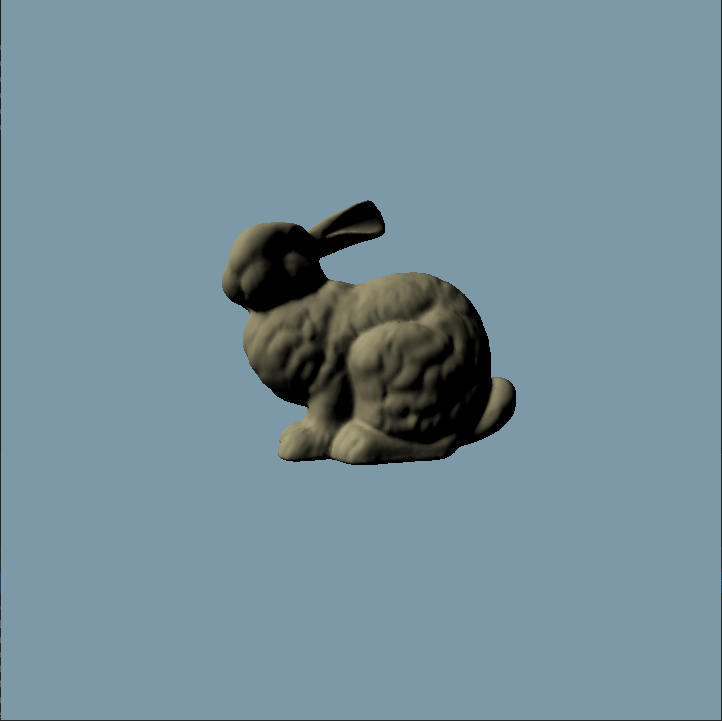
\includegraphics[width=\textwidth]{res/sum_diffuse.png}
        \caption{Światło rozproszone}
        \label{fig:sum_diffuse}
    \end{subfigure}
    ~ %add desired spacing between images, e. g. ~, \quad, \qquad, \hfill etc. 
    %(or a\,blank line to force the subfigure onto a\,new line)
    \begin{subfigure}[b]{0.3\textwidth}
        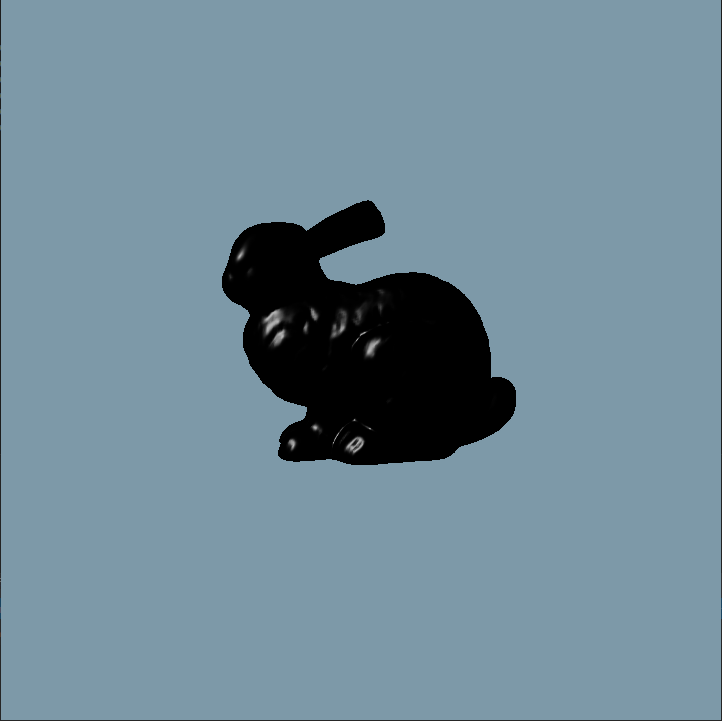
\includegraphics[width=\textwidth]{res/sum_specular.png}
        \caption{Światło zwierciadlane}
        \label{fig:sum_specular}
    \end{subfigure}
    ~ %add desired spacing between images, e. g. ~, \quad, \qquad, \hfill etc. 
    %(or a\,blank line to force the subfigure onto a\,new line)
    \begin{subfigure}[b]{0.3\textwidth}
        
\includegraphics[width=\textwidth]{res/sum_ambient.png}
        \caption{Światło otoczenia}
        \label{fig:sum_ambient}
    \end{subfigure}
    ~ %add desired spacing between images, e. g. ~, \quad, \qquad, \hfill etc. 
    %(or a\,blank line to force the subfigure onto a\,new line)
    \begin{subfigure}[b]{0.5\textwidth}
        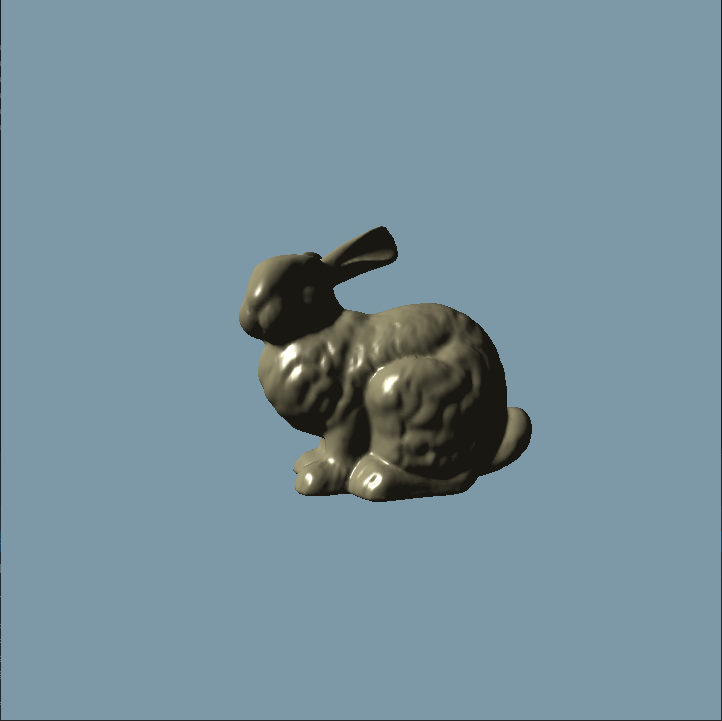
\includegraphics[width=\textwidth]{res/sum_lights.png}
        \caption{Nałożenie świateł}
        \label{fig:sum_lights}
    \end{subfigure}
    \caption{Model oświetlenia}
    \label{fig:sum_comparasion}
\end{figure}

\subsubsection{Generacja terenu}
Do wyświetlania terenu przygotowany został osobny mechanizm renderujący oraz jednostki cieniujące. Jego siatka, w~odróżnieniu od standardowych obiektów, jest prosta, regularna i~powtarzalna, dzięki czemu można ją w~prosty sposób wygenerować bezpośrednio w~programie. Jej schemat został przedstawiony na rysunku \ref{fig:terrain_grid}. \\
Każdy wierzchołek siatki terenu zawiera takie same elementy jak każdy inny obiekt:
\begin{itemize}
    \item wektor współrzędnych,
    \item wektor zmapowanych współrzędnych tekstur,
    \item wektor normalny.
\end{itemize}

\begin{figure}[H]
    \centering
    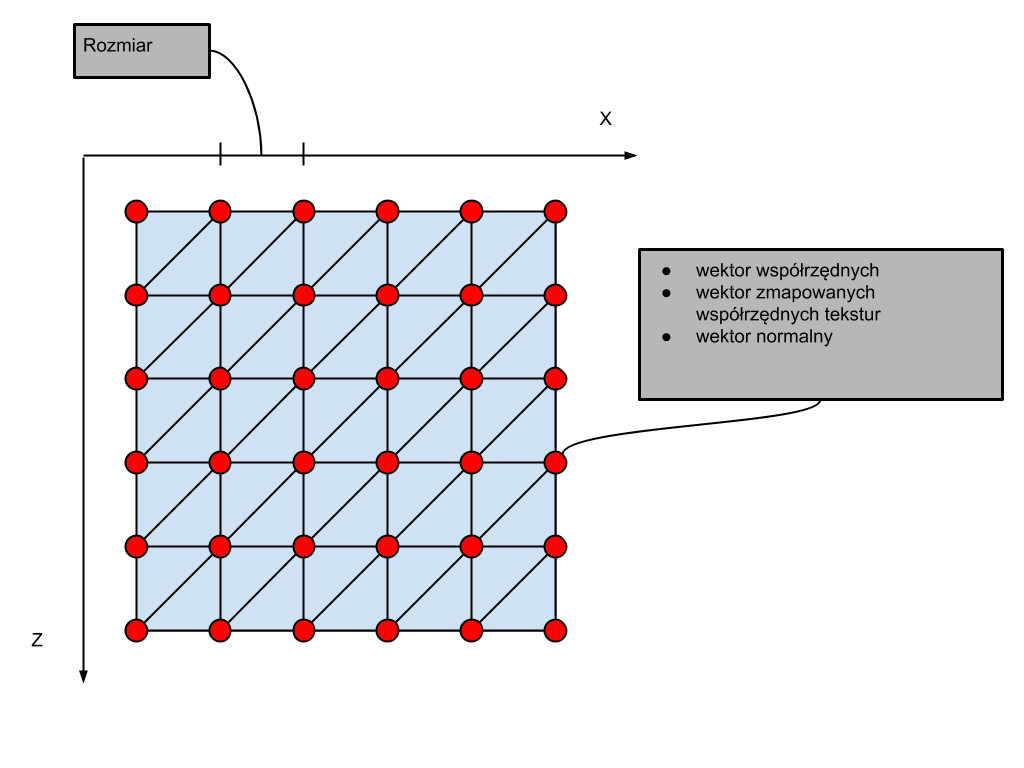
\includegraphics[width=\textwidth]{res/terrain_grid.png}
    \caption{Siatka terenu}
    \label{fig:terrain_grid}
\end{figure}

Generacja terenu polega na utworzeniu czterech tablic, zawierających wyżej wymienione atrybuty oraz tablicy indeksów wierzchołków tworzących trójkąty. Program przechodzi po każdym wierzchołku i~oblicza potrzebne parametry na podstawie zmiennych podstawowych, takich jak: rozmiar, liczba wierzchołków, maksymalna i~minimalna wysokość oraz map wysokości i~map mieszania. Iteracja odbywa się dwukrotnie, za drugim razem wypełniana zostaje tablica indeksów, a~za pierwszym pozostałe parametry. %Całkowity proces generacji terenu obrazuje listing \ref{terrain-gen}. 

%\lstinputlisting[language=c++, caption=Proces generacji terenu, label=terrain-gen]{res/terrain_gen.txt}

Należy również wspomnieć, że do wyliczenia normalnych wierzchołków wykorzystana została metoda różnic skończonych, wykorzystująca dane sąsiednich wierzchołków.

\lstinputlisting[language=c++, caption=Obliczenie wektora normalnego, label=terrain-normal]{res/terrain_normal.txt}

Po utworzeniu wszystkich potrzebnych tablic, zostają one wczytane do VAO, skąd są gotowe do pracy z~OpenGL.

\vspace{\baselineskip}
\textbf{$\bullet$ Mapa wysokości} \\
Do ustalenia wysokości terenu w~danym punkty wykorzystywana jest mapa wysokości. Przyjmuje formę obrazu rastrowego w~skali szarości, zapisanego w~formacie \texttt{.png}. Każdy piksel przechowuje wartości, na podstawie których wyliczona zostaje wysokość na scenie. Im wyższa ta wartość (jaśniejszy piksel) tym wyżej znajduje się dany obszar. W~podstawowej wersji aplikacji badawczej wykorzystywane są mapy wysokości o~wymiarach 256 x 256 pikseli, co daje możliwość zapisu 65536 różnych wartości wysokości. Rysunek \ref{fig:terrain_heightexample} przedstawia efekt zastosowania tej metody.

\begin{figure}[H]
    \centering
    \begin{subfigure}[b]{0.4\textwidth}
        
\includegraphics[width=\textwidth]{res/height_map.png}
        \caption{Przykładowa mapa wysokości}
        \label{fig:height_map}
    \end{subfigure}
    ~ %add desired spacing between images, e. g. ~, \quad, \qquad, \hfill etc. 
    %(or a\,blank line to force the subfigure onto a\,new line)
    \begin{subfigure}[b]{0.55\textwidth}
        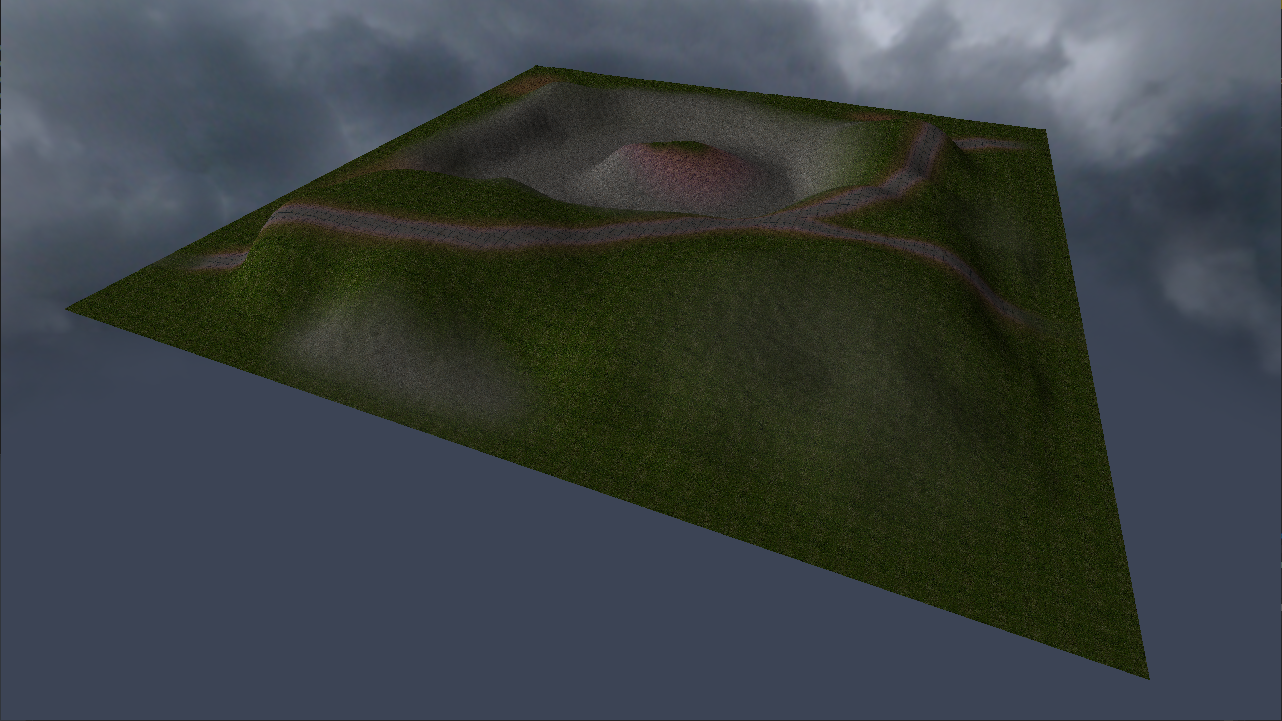
\includegraphics[width=\textwidth]{res/terrain_example.png}
        \caption{Efekt na scenie}
        \label{fig:terrain_example}
    \end{subfigure}
    \caption{Mapa wysokości - przykład}
    \label{fig:terrain_heightexample}
\end{figure}



Wartość koloru piksela nie może być ujemna i~może osiągać bardzo duże liczby, co byłoby problematyczna przy budowie sceny. Wyznaczenie pożądanej wysokości zostało zrealizowane poprzez zdefiniowanie stałej maksymalnej wartości i~uzależnienie od niej zakresu dostępnych danych. To przekształcenie zostało zilustrowane na rysunku \ref{fig:terrain_heighttransform} oraz listingu \ref{terrain-getheight}.

\lstinputlisting[language=c++, caption=Obliczenie wysokości terenu w~punkcie, label=terrain-getheight]{res/terrain_getheight.txt}

\begin{figure}[H]
    \centering
    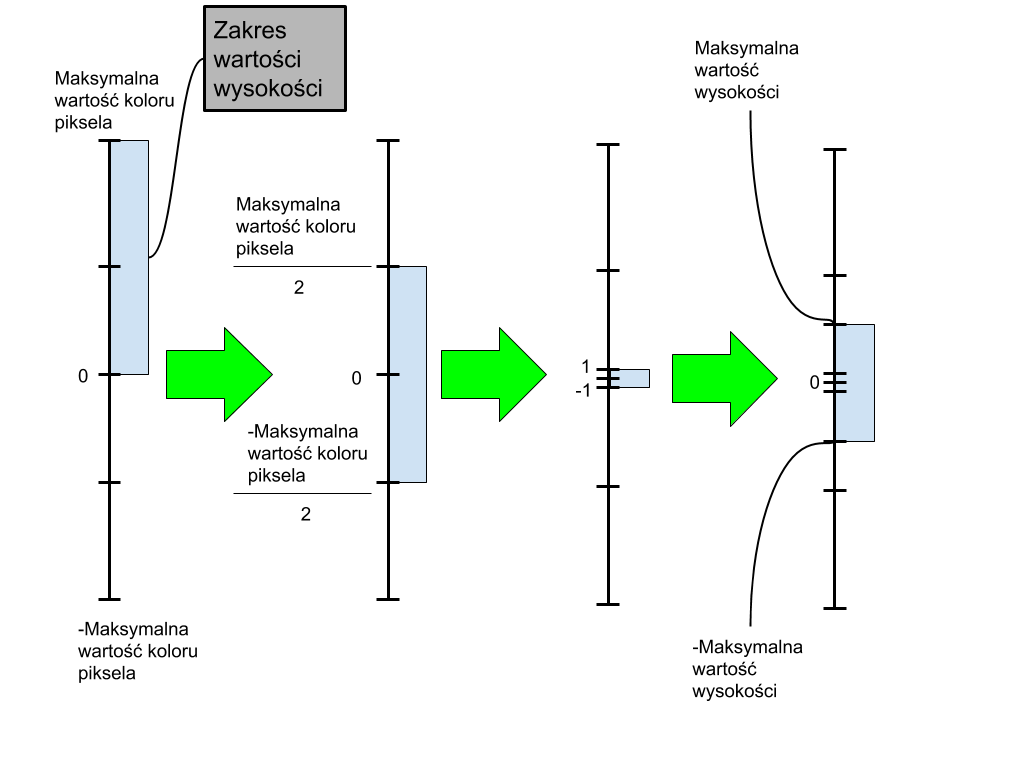
\includegraphics[width=1.2\textwidth]{res/terrain_heighttransform.png}
    \caption{Przekształcenie koloru piksela na wartość wysokości}
    \label{fig:terrain_heighttransform}
\end{figure}


\vspace{\baselineskip}
\textbf{$\bullet$ Mieszanie tekstur} \\
Mapa mieszania - obraz w~modelu RGB, gdzie nasycenia poszczególnych kolorów odpowiadają widoczności wskazanej tekstury. W~pracy zostały wykorzystane obrazy o~wymiarach 256 x 256 pikseli oraz 4 kolory: czerwony, zielony, niebieski oraz czarny. Kolor czarny odpowiada teksturze podstawowej, widocznej gdy żadna inna nie jest używana w~danym obszarze.

\begin{figure}[H]
    \centering
    \begin{subfigure}[b]{0.475\textwidth}
        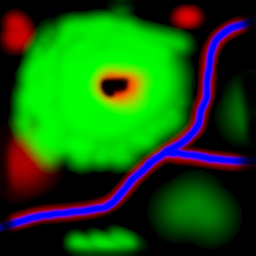
\includegraphics[width=\textwidth]{res/blend_map.png}
        \caption{Przykładowa mapa mieszania}
        \label{fig:blend_map}
    \end{subfigure}
    ~ %add desired spacing between images, e. g. ~, \quad, \qquad, \hfill etc. 
    %(or a\,blank line to force the subfigure onto a\,new line)
    \begin{subfigure}[b]{0.475\textwidth}
        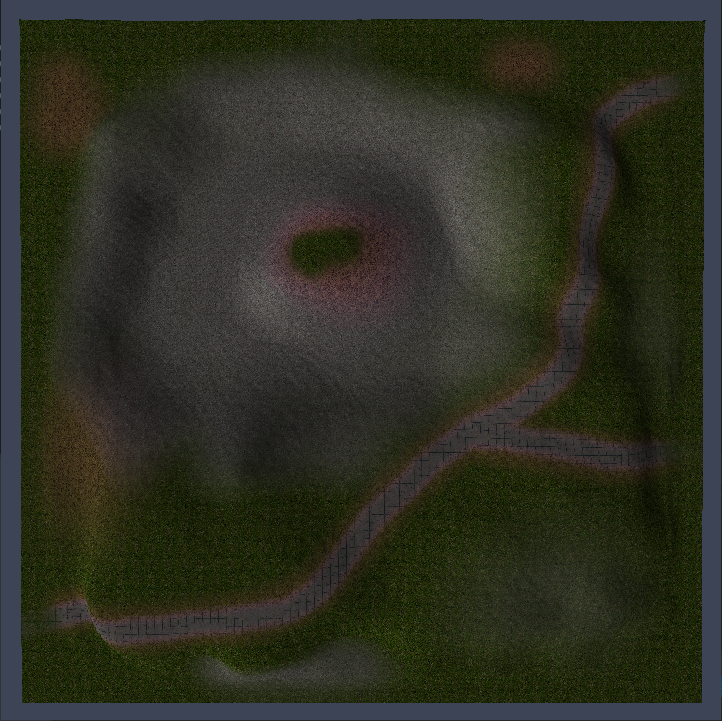
\includegraphics[width=\textwidth]{res/terrain_blend.png}
        \caption{Efekt na scenie}
        \label{fig:terrain_blend}
    \end{subfigure}
    \caption{Mapa mieszania - przykład}
    \label{fig:blend_example}
\end{figure}

Jak widać na rysunkach \ref{fig:blend_example} mieszanie tekstur można wykorzystać do utworzenia różnych rodzajów terenu z~wykorzystaniem grafik o~małym rozmiarze. OpenGL posiada wiele jednostek, w~których można przechowywać informacje o~teksturach. Pożądany efekt został zrealizowany poprzez wczytanie wszystkich potrzebnych tekstur oraz mapy mieszania do osobnych jednostek, a~następnie w~jednostce cieniującej fragmentów terenu kolor tekstury jest wybierany zgodnie z~informacjami zawartymi na mapie mieszania. Proces został przedstawiony na listingu \ref{blend-frag}. \\
Należy zwrócić uwagę na łagodne przejścia między poszczególnymi teksturami, jak można osiągnąć stosując tę technikę. Kolor w~modelu RGB posiada trzy składowe przez co możliwe staje się pobranie części koloru z~jednej tekstury i~drugiej z~innej.

\lstinputlisting[language=c++, caption=Mieszanie tekstur w~jednostce fragmentów terenu, label=blend-frag]{res/blend_frag.txt}

\subsubsection{Generacja panoramy sceny (ang. \ang{Skybox})}
Metoda wykorzystana do utworzenia tła sceny sprowadza się do utworzenia dużego sześcianu, zaopatrzonego w~tekstury widoczne od środka. Środek obiektu wyznacza pozycja kamery. \\
Do zapisu wymaganej tekstury użyta została struktura OpenGL - Sześcienna Mapa Tekstury (ang. \ang{Texture Cube Map}). Obiekt podzielony jest na sześć sekcji, każda z~nich reprezentuje jedną ścianę kostki. Pozwala to zaoszczędzić miejsce - zamiast sześciu tekstur została wykorzystana tylko jedna. Rysunek \ref{fig:skybox_example} pokazuje grafiki składowe tekstury oraz efekt na scenie.

\begin{figure}[H]
    \centering
    \begin{subfigure}[b]{0.475\textwidth}
        
\includegraphics[width=\textwidth]{res/skybox_texture.png}
        \caption{Przykładowa tekstura panoramy}
        \label{fig:skybox_texture}
    \end{subfigure}
    ~ %add desired spacing between images, e. g. ~, \quad, \qquad, \hfill etc. 
    %(or a\,blank line to force the subfigure onto a\,new line)
    \begin{subfigure}[b]{0.475\textwidth}
        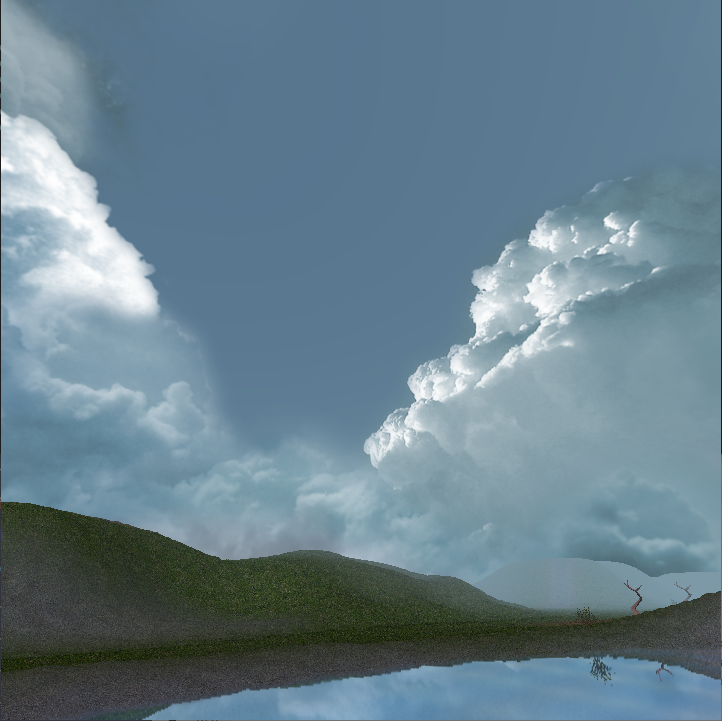
\includegraphics[width=\textwidth]{res/skybox_scene.png}
        \caption{Efekt na scenie}
        \label{fig:skybox_scene}
    \end{subfigure}
    \caption{Panorama sceny - przykład}
    \label{fig:skybox_example}
\end{figure}

\textbf{Efekt mgły} - dodatkowo w~jednostkach cieniujących fragmentów zaimplementowany został efekt wtapiania się elementów sceny w~tło. Wyliczony ostateczny kolor mieszany jest z~barwą podobną do odcienia tekstury dalszego planu. Dzięki temu zabiegowi obiekty na scenie są coraz mniej widoczne i~zostają przygotowane do pracy z~technikami optymalizacyjnymi.

\subsubsection{Symulacja wody}
Symulacja wody jest złożonym procesem, na który składa się wiele mechanizmów i~struktur. Celem tej pracy nie jest jednak ich analiza, dlatego zostaną one opisane bez większego zagłębiania w~szczegóły implementacji. \\
Aby prawidłowo zrealizować zadanie konieczna była implementacja technik imitujących zjawiska fizyczne, które opisują zachowanie się wody. 
\begin{itemize}
    \item Refrakcja i~odbicie - ustalana jest płaszczyzna przycinająca (ang. \ang{clip plane}), która dzieli całą scenę na obszar znajdujący się powyżej tafli wody oraz poniżej. Następnie utworzone zostają dwa FBO \footnote{FBO (ang. \ang{Frame Buffer Object}) - Obiekt Bufora Klatki - obiekty OpenGL, umożliwiające renderowanie do niedomyślnych lokalizacji bufora klatki, to znaczy bez zakłócania ekranu głównego.} (ang. \ang{Frame Buffer Object}). Na pierwszy z~nich renderowany jest widok z~kamery o~niezmienionej pozycji, ale obcięty o~wszystko ponad płaszczyzną przycinającą. Drugi FBO przechowuje widok z~kamery analogicznie spoglądającej w~stronę tafli wody, jednak przesuniętej w~dół o~wartość odpowiadającą dwukrotnej wysokości pierwotnej kamery. W~tym przypadku kamera nie widzi obszaru położonego poniżej płaszczyzny przycinającej. Na koniec obrazy z~obu FBO nakładane są na taflę wody, dodany zostaje delikatny kolor niebieski oraz inne efekty.
    \item Efekt Fresnela - decyduje o~stosunku odbicia do refrakcji. Patrząc na wodę z~góry użytkownik powinien bez przeszkód zobaczyć dno zbiornika, podczas gdy patrząc pod niewielkim kątem należy spodziewać się, że odbicie będzie bardzo wyraźne. Efekt został przedstawiony na rysunku \ref{fig:water_fresnel}.
    
    \begin{figure}[H]
        \centering
        \begin{subfigure}[b]{0.475\textwidth}
            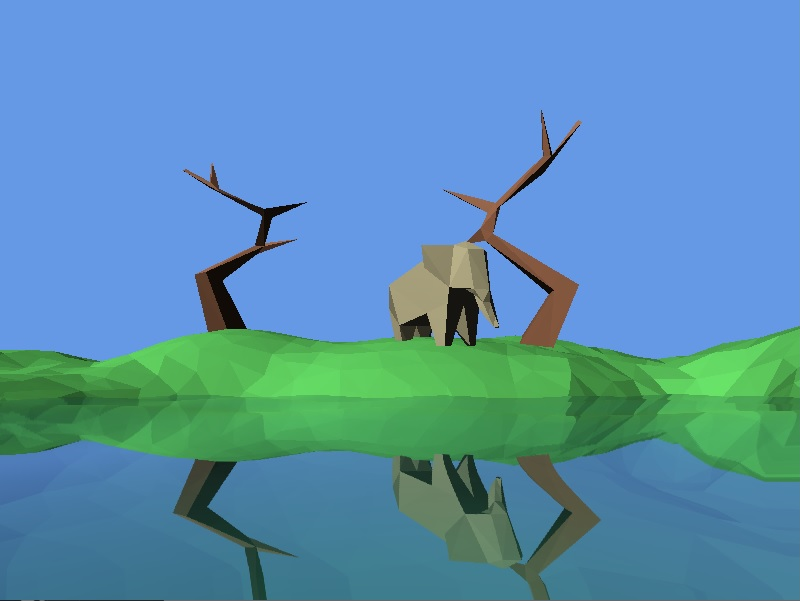
\includegraphics[width=\textwidth]{res/water_fresnel1.png}
            \label{fig:water_fresnel1}
        \end{subfigure}
        ~ %add desired spacing between images, e. g. ~, \quad, \qquad, \hfill etc. 
        %(or a\,blank line to force the subfigure onto a\,new line)
        \begin{subfigure}[b]{0.475\textwidth}
            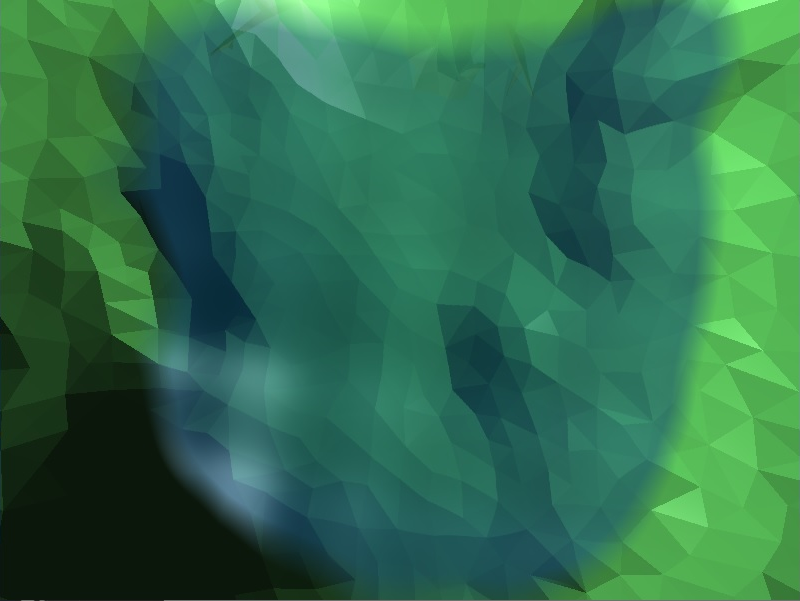
\includegraphics[width=\textwidth]{res/water_fresnel2.png}
            \label{fig:water_fresnel2}
        \end{subfigure}
        \caption{Efekt Fresnela}
        \label{fig:water_fresnel}
    \end{figure}

    \item Efekt mętnej wody - utworzona została mapa głębokości zbiornika wody. Na jej podstawie dodany kolor niebieski jest coraz bardziej intensywny w~niżej położonych obszarach. Nadaje to efekt mętności, w~głębinach trudniej jest dostrzec odbicia i~refrakcji. Do uzyskania tego efektu wykorzystana została mapa głębokości (rysunek \ref{fig:water_depth}) - im jaśniejszy kolor tym głębiej.
    
    \begin{figure}[H]
        \centering
        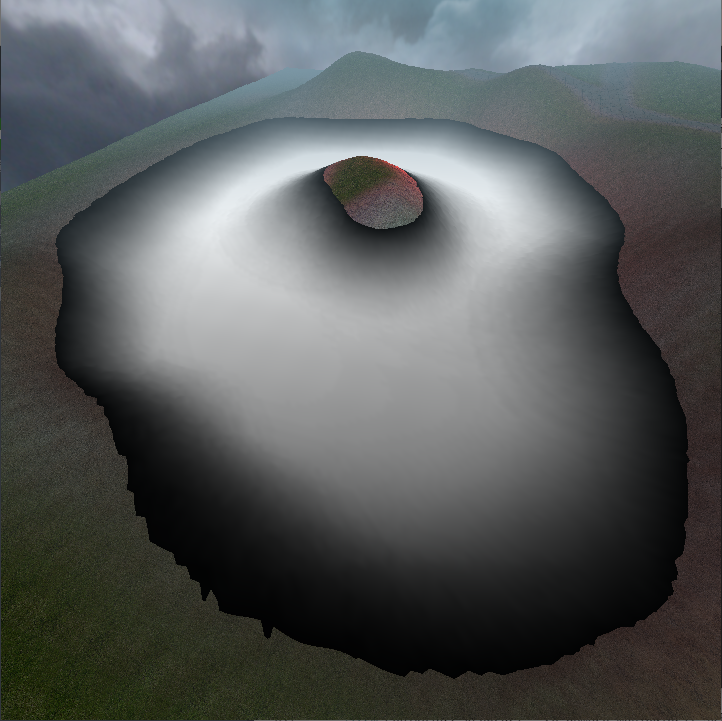
\includegraphics[width=0.6\textwidth]{res/water_depth.png}
        \caption{Mapa głębokości}
        \label{fig:water_depth}
    \end{figure}
    
    \item Zanikające krawędzi - za pomocą manipulacji składowej alfa koloru wody, staje się ona coraz mnie widoczna przy brzegach zbiornika.
    \item Mapy DUDV - w~celu wprawienia wody w~ruch zastosowane zostały dwie metody. Jedna z~nich to mapy DUDV. Z~wczytanych tekstur pobierane są wartości nasycenia kolorów zielonego i~czerwonego, na podstawie których nakładane na wodę zostają zniekształcenia. Tekstura przesuwana jest po tafli wody w~czasie, dzięki czemu woda zdaje się być w~ruchu. Ta technika wykorzystywana jest dla tafli wody o~bardzo prostej siatce wierzchołków - kwadratu, składającego się z~dwóch trójkątów, na który nałożone zostają wszystkie efekty. Metoda jest prosta i~wydajna, ale jej możliwości są ograniczone.
    \item Poruszanie wierzchołków - drugą metodą wprawienia tafli wody w~ruch jest manipulacja siatką wierzchołków, złożoną tym razem z~wielu trójkątów. Struktura generowana jest w~podobny sposób jak siatka terenu. Ruch wierzchołków realizowany jest w~jednostce cieniującej wierzchołków. Jak widać na rysunku \ref{fig:water_vertices} powierzchnia wody składa się z~wielu wierzchołków, co jest bardziej obciążające dla geometrycznego etapu potoku renderującego. Wymagane są tutaj również dodatkowe obliczenia i~zmienne w~jednostkach cieniujących. Mimo to ze względu na bardzo szerokie możliwości tej metody warto z~niej korzystać i~to właśnie ja została użyta w~testach przeprowadzonych w~ramach tej pracy.
    
    \begin{figure}[H]
        \centering
        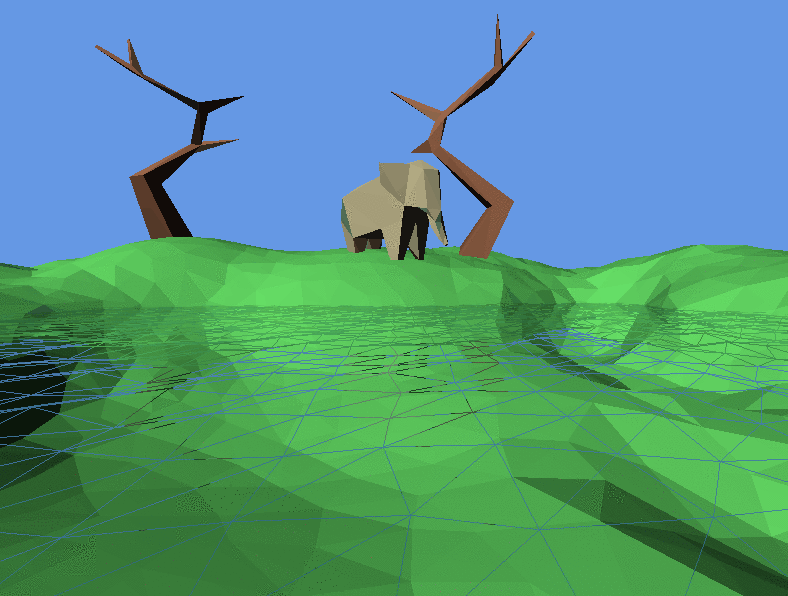
\includegraphics[width=0.6\textwidth]{res/water_vertices.png}
        \caption{Ruchoma siatka wody}
        \label{fig:water_vertices}
    \end{figure}
    
\end{itemize}

\subsubsection{Obsługa wielu źródeł światła, w~tym świateł punktowych}
Obsługa wielu źródeł światła sprowadza się do utworzenia struktury zdolnej do ich przechowywania i~wczytania do środowiska OpenGL oraz zmiany kodu jednostek cieniujących. Zmiany tez zostały przedstawione w~listingu \ref{multilight-frag} na przykładzie jednostki cieniującej fragmentów obiektów. 

\lstinputlisting[language=c++, caption=Jednostka cieniująca fragmentów obiektów - obsługa wielu punktowych źródeł światła, label=multilight-frag]{res/multilight_frag.txt}

Jak widać wszystkie obliczenia wykonywane są tyle razy ile źródeł światła znajduje się na scenie, a~ich wyniki sumowane. Sam proces niewiele różni się od standardowych obliczeń przedstawionych w~modelu oświetlenia. Światło otoczenia musi zostać wyliczone na samym końcu poza pętlą iteracyjną, ponieważ należy dodać je tylko raz, niezależnie od liczby źródeł światła.\\
W wyliczeniach pojawia się również zmienna \texttt{attFactor} zależna od \texttt{attenuation} (z angielskiego tłumienie, osłabianie). Jest to nowy parametr źródła światła, zawierający dane o~zasięgu światła i~stopniu jego zanikania wraz ze zwiększaniem odległości od jego pozycji. Uzyskany efekt ilustruje rysunek \ref{fig:multilight_example}.

\begin{figure}[H]
    \centering
    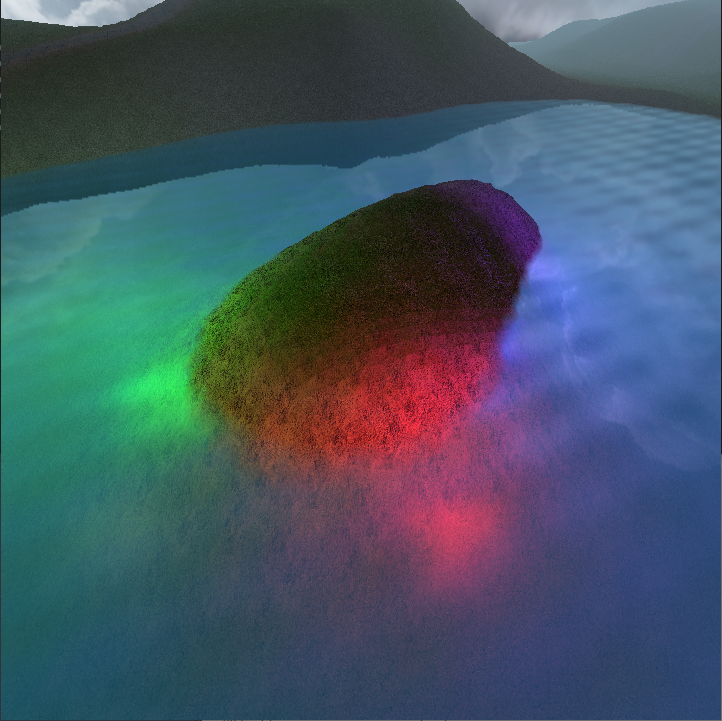
\includegraphics[width=0.6\textwidth]{res/multilight_example.png}
    \caption{Przykład wielu punktowych źródeł światła}
    \label{fig:multilight_example}
\end{figure}


\subsubsection{Obsługa kamery}
Do swobodnego przemieszczania się po scenie zaimplementowana została podstawowa obsługa kamery, korzystająca z~klawiatury i~myszy. Funkcjonalność używa wielu funkcji pomocniczych biblioteki GLFW. W~ramach pracy kamera może:
\begin{itemize}
    \item zmieniać swój kąt obrotu wokół trzech osi, zgodnie z~układem przestrzeni euklidesowej,
    \item przemieszczać się w~dół, górę, lewo, prawo, przód, tył,
    \item przyspieszyć w kierunku zwrotu kamery.
\end{itemize}
W ramach silnika nie została zaimplementowana obsługa kolizji, co wiąże się z~możliwością przejścia kamery przez tekstury sceny. \\
Program umożliwia zmianę czułości ruchów poprzez odpowiednie stałe.

\section{Narzędzia zewnętrzne}
Do konstrukcji scen, w~tym utworzenia modeli i~tekstur obiektów wykorzystane zostały następujące narzędzia zewnętrzne:
\begin{itemize}
    \item Blender 2.80 - pakiet do tworzenia grafik 3D, który oferuje szeroki zakres narzędzi, w~tym modelowanie, renderowanie, animacja, edycja wideo, efekty wizualne, komponowanie, teksturowanie i~wiele rodzajów symulacji. Jest wieloplatformowy i posiada interfejs graficzny oparty o~OpenGL. Można go dostosować za pomocą skryptów Python. Oprogramowanie jest na licencji otwartoźródłowej (ang. \ang{open source}), co oznacza, że korzystanie z~niego jest darmowe oraz użytkownik ma prawo do modyfikowania własnej kopii programu. \cite{bib:blender}
    \item GIMP 2.10.8 (ang. \ang{GNU Image Manipulation Program}) - program GNU (ang. \ang{GNU Not Unix}) do manipulacji obrazami, jest programem przeznaczonym do tworzenia i~edycji obrazów bitmapowych. Oznacza to, że nadaje się zarówno do edycji zdjęć cyfrowych jak i~typowej grafiki komputerowej. Często wykorzystywany jest również do tworzenia własnych obrazów. \\
    Program jest darmowym oprogramowaniem na licencji otwartoźródłowej: nie trzeba za niego płacić, aby z~niego korzystać, a~kod źródłowy jest dostępny dla każdego, kto chce go zbadać, przyczyniać się do jego rozwoju, rozpowszechniać lub uczyć się z~niego. \cite{bib:gimp}
\end{itemize}

\vbox{}

Do pomiaru wartości wskaźników wydajności użyty zostały program pomocniczy:
\begin{itemize}
    \item FPS Monitor - narzędzie przeznaczone do śledzenia stan sprzętu komputera i~wyświetlania tych informacji w~postaci nakładki na okno programu. Interfejs jest modyfikowalny i~zapewnia wgląd do wielu parametrów, takich jak liczba klatek na sekundę, obciążenie procesora czy karty graficznej. \\
    Oprogramowanie jest płatne, ale producent udostępnia darmowe demo aplikacji, które zostało wykorzystane w~ramach pracy. \\
    Na rysunku \ref{fig:fps_monitor} przedstawiono przykład działania programu.
    \begin{figure}[H]
        \centering
        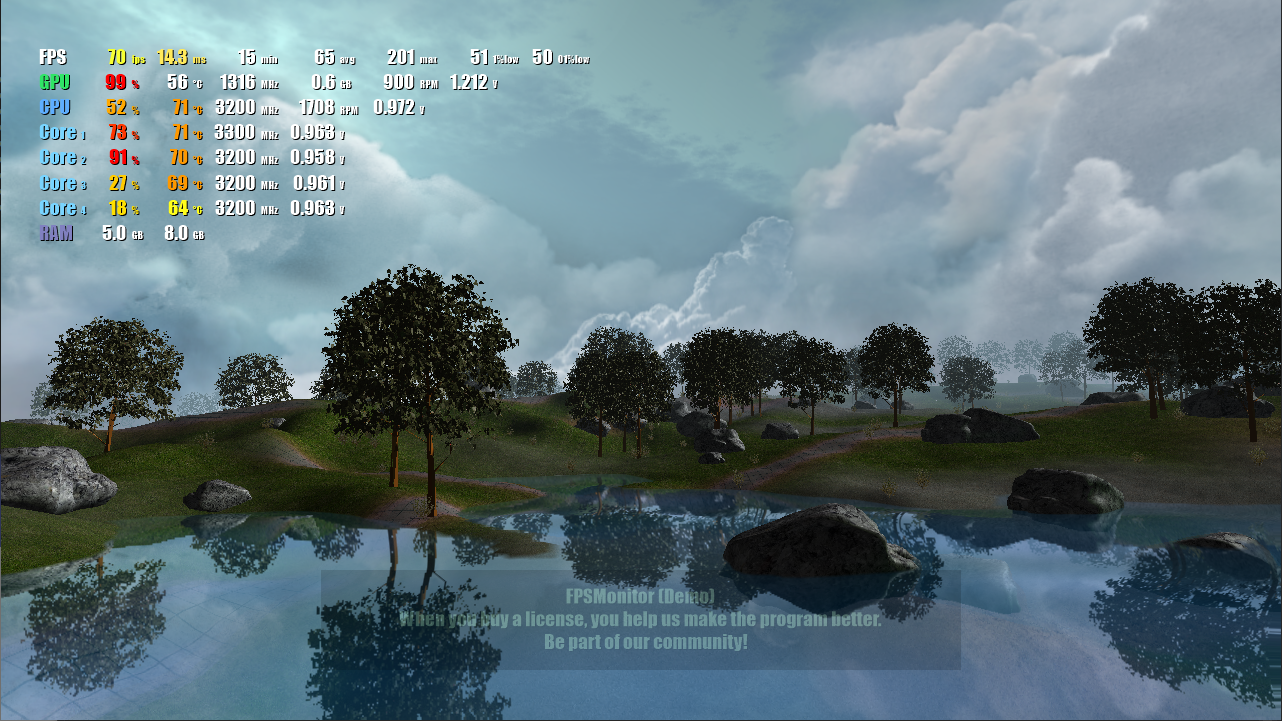
\includegraphics[width=0.8\textwidth]{res/fps_monitor.png}
        \caption{Przykład działania programu FPS Monitor}
        \label{fig:fps_monitor}
    \end{figure}
\end{itemize}

\section{Opis scen}
Do przeprowadzenia testów utworzone zostały dwie różne sceny podstawowe, przy czym każda z~nich występuje w~wielu wariantach w~zależności od aktualnie badanych parametrów. W~ramach aplikacji badawczej elementy sceny zostały podzielone na pięć grup:
\begin{itemize}
    \item Obiekty - podstawowe składniki obrazu, zapisywane przy pomocy plików \texttt{.obj}. Zazwyczaj reprezentują elementy krajobrazu takie jak drzewa, skały czy zwierzęta.
    \item Teren - podłoże, na którym umieszczane są obiekty.
    \item Woda - na ustalonej wysokości renderowana jest tafla wody. Poprawna obsługa tego elementu wymaga dużych zasobów silnika.
    \item Światła - podstawa modelu oświetlania sceny, regulują natężenie kolorów pozostałych elementów.
    \item Panorama - tło sceny - stały obraz, niewchodzący w~interakcję z~pozostałymi elementami.
\end{itemize}
Każdy z~tych elementów posiada własną jednostkę renderującą, zestaw jednostek cieniujących oraz struktury odpowiadające za ich obsługę. \\
W ramach badań wstępnych stwierdzono, że testy dadzą bardziej miarodajne wyniki, gdy zostaną przeprowadzone na mniejszej liczbie scen. Takie podejście pozwala na pomiar wpływu metod optymalizacyjnych w~takim samym środowisku. Większa liczba scen teoretycznie pozwoliłaby na dokładniejsze zbadanie poszczególnych czynników pracy silnika, ale z~drugiej strony trudniejszym zadaniem stałoby się stwierdzenie czy zmiana wyników nastąpiła przez wpływ badanej metody czy przez zmianę środowiska badawczego. Niemniej jednak, w~celu ściślejszej analizy odrębnych technik zwiększających wydajność, wprowadzono warianty scen, które umożliwiają zmianę parametrów środowiskowych, przy jednoczesnym zachowaniu tych samych elementów otoczenia.

\subsection{Scena 1 - Krajobraz}
Pierwsza scena ma odpowiadać scenerii naturalnej, imitującej w~pewnym stopniu naturalne środowisko. Wykorzystuje ona wszystkie dostępne grupy elementów sceny. Na płaszczyźnie, określonej przez 16 tafli terenu o~wymiarach 100 x 100 jednostek, losowo rozkładane są różne obiekty, takie jak: drzewa, trawy czy skały. Jeżeli teren zejdzie poniżej pewnego poziomu odkryta zostaje tafla wody. W~tle widać panoramę sceny w~formie sześciennej tekstury. Przykład sceny przedstawiono na rysunku \ref{fig:scene1_example}. \\

\begin{figure}[H]
    \centering
    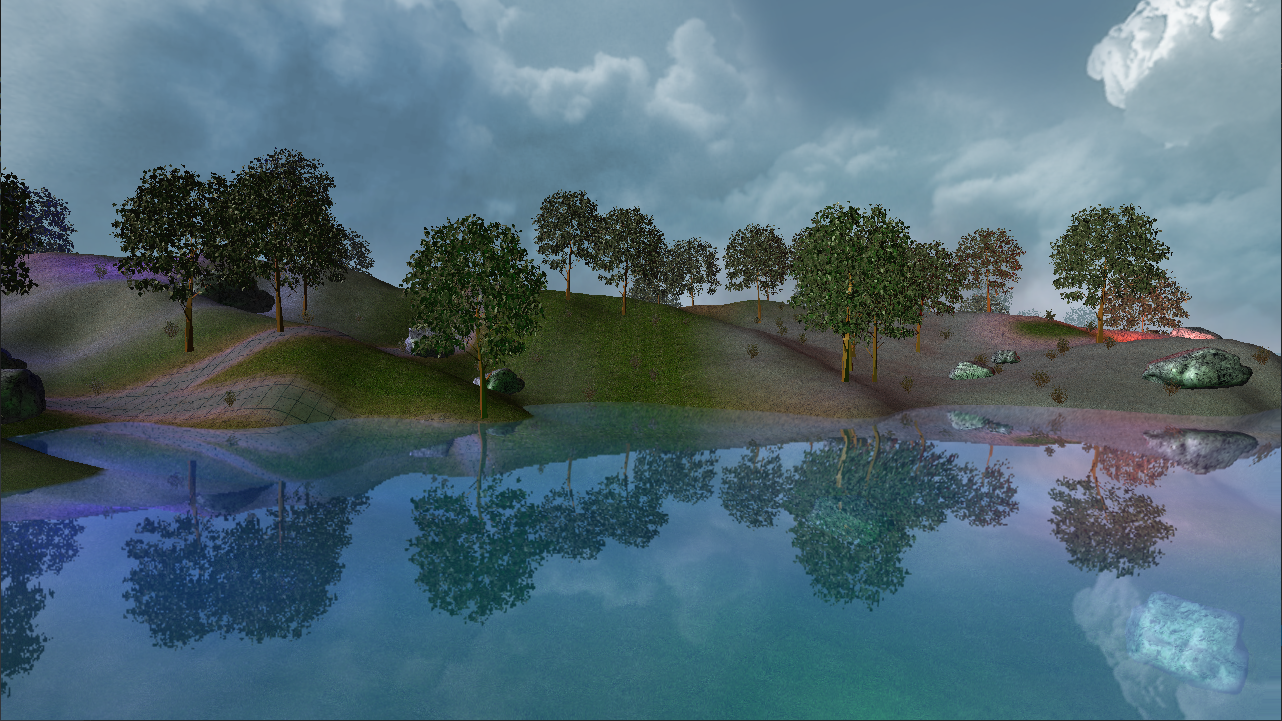
\includegraphics[width=0.9\textwidth]{res/scene1_example.png}
    \caption{Przykład sceny krajobrazu}
    \label{fig:scene1_example}
\end{figure}

Scena pozwala na zbadanie wpływu każdej z~metod na elementy z~każdej grupy składników sceny. W~prosty sposób można zmienić parametry sceny lub dodać czy wykluczyć dowolny zestaw elementów z~procesu renderowania, aby skupić się na wybranych aspektach pracy silnika. \\
Warianty tej sceny przewidują:
\begin{itemize}
    \item modele obiektów o~mniej lub bardziej złożonej strukturze,
    \item zmienną liczbę obiektów,
    \item zmienną wielkość wykorzystanych tekstur.
\end{itemize}

\vbox{}

Stałe pozostają:
\begin{itemize}
    \item liczba źródeł światła = 4,
    \item wykorzystanie powierzchni i~jednostek renderujących wody = 1 duża tafla,
    \item wykorzystanie powierzchni i~jednostek renderujących teren = 16 mniejszych powierzchni,
    \item wykorzystanie panoramy sceny.
\end{itemize}

\subsection{Scena 2 - Chmura obiektów}
Druga scena służy głównie do pracy z~dużą liczbą bytów. Wyznaczony zostaje obszar, w~ramach którego generowane są obiekty w~losowych pozycjach. Nie przewidziano zastosowania tutaj elementów z~innych grup, poza panoramą otoczenia i~źródłami światła. Przykład takiej sceny przedstawiono na rysunku \ref{fig:scene2_example}.

\begin{figure}[H]
    \centering
    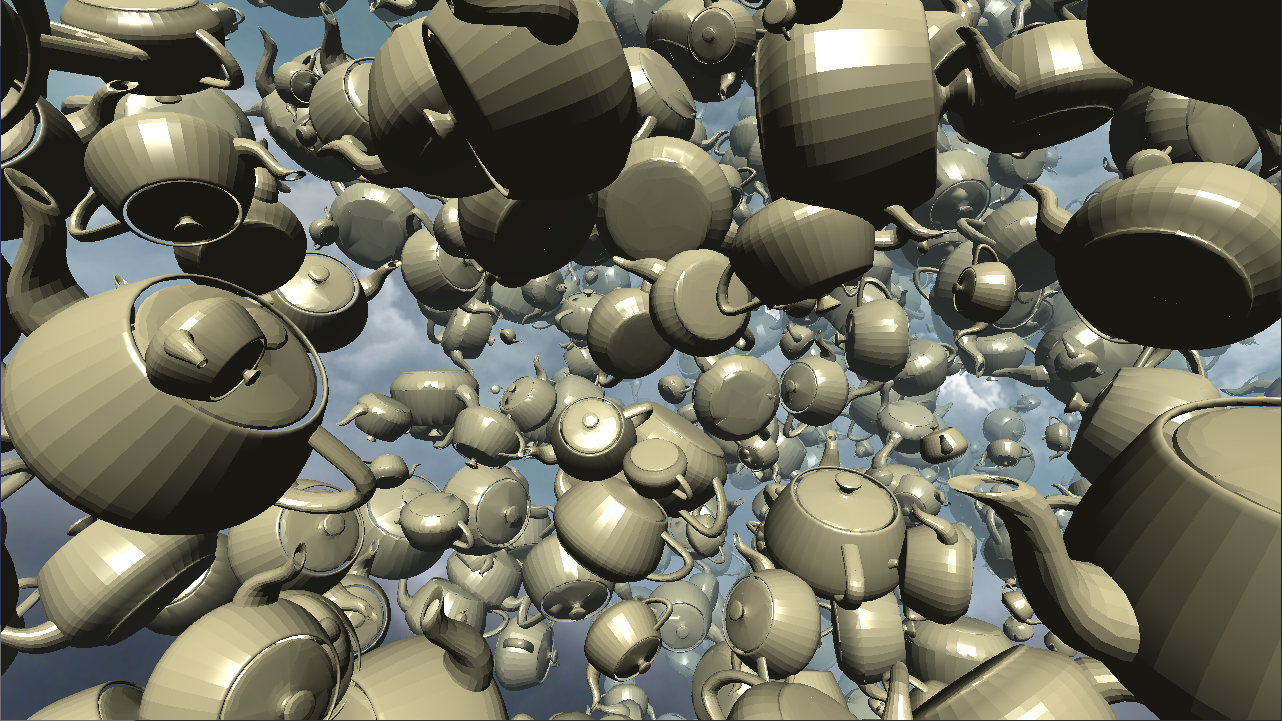
\includegraphics[width=0.9\textwidth]{res/scene2_example.png}
    \caption{Przykład sceny chmury obiektów}
    \label{fig:scene2_example}
\end{figure}

Scena pozwala na bardziej jednostkowe podejście. Możliwe jest wyizolowanie poszczególnego obiektu i~zbadanie każdego z~czynników jaki może wpływać na wydajność jego renderowania. Przykładami może być zmiana tekstury danego obiektu czy zmniejszenie liczby jego wierzchołków. \\

Warianty tej sceny przewidują:
\begin{itemize}
    \item modele obiektów o~mniej lub bardziej złożonej strukturze,
    \item zmienną liczbę obiektów,
    \item zmienną wielkość wykorzystanych tekstur.
\end{itemize}

\vbox{}
\vbox{}

Stałe pozostają:
\begin{itemize}
    \item liczba źródeł światła = 1,
    \item wykorzystanie powierzchni i~jednostek renderujących wody = brak,
    \item wykorzystanie powierzchni i~jednostek renderujących teren = brak,
    \item wykorzystanie panoramy sceny.
\end{itemize}

\section{Wykorzystane wskaźniki wydajności}
\label{section:benchamarks}
Wartości zbierane w~testach, na podstawie których przeprowadzona została analiza wydajności to:
\begin{itemize}
    \item Liczba klatek na sekundę - częstotliwość, z~jaką na ekranie pojawiają się kolejne obrazy, jest uważana za szybkość renderowania. Jedna klatka wymaga wyrysowania i~obsługi wszystkich widocznych obiektów sceny. Bardziej dokładny pomiar można uzyskać, mierząc czas wielu klatek. Na potrzeby analizy z~każdego testu dynamicznego zebrano średnią, maksymalna i~minimalną liczbę klatek na sekundę.
    \item Czas trwania jednej klatki - odwrotność liczby klatek na sekundę, która to nie zawsze jest najlepszym sposobem pomiaru wydajności, ponieważ jest to wartość zmieniająca się nieliniowo w~dziedzinie czasu. W~celu wyjaśnienia problemu przedstawiono dwa przykładowe przypadki:
    \begin{enumerate}[label=(\alph*)]
        \item Na scenę dodano kilka dużych obiektów i~liczba klatek na sekundę zmniejszyła się z~200 na 180. Odnotowano spadek o~20 jednostek, jednak sama ta wartość niewiele mówi, aby sprawdzić o~ile sekund wydłużona została obsługa klatki należy obliczyć czas jej trwania: \\
        \begin{equation}
            1/200 - 1/180 = 0.00056\ sekundy
        \end{equation}
        \item Druga sytuacja ma taki sam przebieg, ale wartość klatek na sekundę zmalała z~30 do 10. Czas trwania jednej klatki został tym samym wydłużony o:
        \begin{equation}
            1/30 - 1/10 = 0.06667\ sekundy
        \end{equation}
    \end{enumerate}
    Chociaż liczba klatek na sekundę spadła w~obu przypadkach o~20, spowolnienie w~pierwszym przypadku nie jest bardzo duże, ale w~drugim przypadku jest zauważalnie większe. \\
    Czas trwania klatki nie jest proporcjonalny do liczby renderowanych obiektów.
    \item Liczba trójkątów na sekundę - zejście na niższy poziom, ta miara może okazać się przydatna przy porównywaniu scen o~wielu nieskomplikowanych obiektach i~scen o~niewielu skomplikowanych obiektach, przyda się również przy badaniu poszczególnych metod zmieniających strukturę modelu.
    \item Liczba renderowanych obiektów - miara określająca ile obiektów na scenie jest aktualnie wyświetlanych i~co za tym idzie obsługiwanych przez potok graficzny. Metody odrzucania elementów powinny obniżać tę wartość.
    \item Liczba renderowanych trójkątów - wszystkie trójkąty wszystkich aktualnie renderowanych elementów, na podstawie tej wartości możliwe staje się nie tylko zbadanie metod manipulacji poziomem detali, ale również porównanie ich do technik odrzucania obiektów.
    \item Obciążenie procesora - miara sprawdzająca stan pracy procesora w~potoku graficznym.
    \item Obciążenie karty graficznej - miara sprawdzająca procent wykorzystania zasobów karty graficznej przez program. Ze względu na brak ograniczeń narzuconych na silnik można się spodziewać, że w~testach zazwyczaj jedna z~wartości: obciążenie procesora lub karty graficznej osiągnie maksymalną wartość 100\% (lub zbliżoną ze względu na inne procesy komputera).
    \item Ilość zajmowanej pamięci - wartość sprawdza ile miejsca potrzebuje program, aby funkcjonować. Głównie wykorzystywana przy rozwoju metod i~aplikacji badawczej, w~celu sprawdzenia wycieków pamięci i~potencjalnych problemów z~rozmiarem danych. Ta miara, obciążenie procesora i~kraty graficznej to standardowe miary pozwalające sprawdzić wpływ aplikacji na sprzęt.
\end{itemize}

\vbox{}

Każda z~dwóch grup testów wykorzystuje nieco inne podzbiory wymienionych wartości:
\begin{itemize}
    \item W~testach statycznych zbierane były:
    \begin{itemize}
        \item średnia liczba wyświetlanych klatek na sekundę,
        \item średni czas trwania klatki,
        \item średnia liczba wyświetlanych trójkątów na sekundę,
        \item średnia liczba wyświetlanych trójkątów w~jednej klatce,
        \item średnia liczba wyświetlanych obiektów w~jednej klatce,
        \item obciążenie procesora,
        \item obciążenie karty graficznej,
        \item ilość zajmowanej pamięci.
    \end{itemize}
    \item W~testach dynamicznych zbierane były:
    \begin{itemize}
        \item średnia liczba wyświetlanych klatek na sekundę,
        \item średni czas trwania klatki,
        \item maksymalny czas trwania klatki,
        \item minimalny czas trwania klatki,
        \item średnia liczba wyświetlanych trójkątów,
        \item średnie czasy trwania dziesięciu kolejnych klatek, na ich podstawie wykreślony został wykres zmian czasu trwania klatek,
        \item średnie liczby wyświetlanych trójkątów w~dziesięciu kolejnych klatkach, na ich podstawie wykreślony został wykres zmian liczby wyświetlanych trójkątów.
    \end{itemize}
\end{itemize}

\vbox{}

W przypadku testów na wersji bazowej silnika, wykres liczby trójkątów jest stały - wartość ta nie zmienia się, ponieważ żadne prymitywy nie są odrzucane z~potoku graficznego. Dlatego w~zestawieniu wyników zostały one pominięte. Podobnie czas trwania klatki został w~tej wersji aplikacji przedstawiony tylko jako wartość średnia.

\section{Środowisko sprzętowe}
Wszystkie testy zostały przeprowadzone na jednym komputerze, z~użyciem tych samych podzespołów oraz tego samego systemu operacyjnego. \\
Środowisko sprzętowe prezentuje się następująca:
\begin{itemize}
    \item System operacyjny: Microsoft Windows 10 Pro 64-bit
    \item Karta graficzna: NVIDIA GeForce GTX 960, 2GB RAM
    \item Procesor: Intel Core i5-4460 3.20GHz, 4 rdzenie, 4 procesory logiczne
    \item Pamięć RAM: Crucial DDR3, 8 GB, 1600MHz
\end{itemize}

\newpage

\section{Wyniki}
\label{section:wyniki}

\subsection{Odrzucanie tylnych ścian}

\subsubsection{Test 1.1}
\begin{tabular}{|l||l|}
\hline
Numer sceny: & 1 \\
\hline
Typ testu: & statyczny \\
\hline
Cechy szczególne: & standard \\
\hline
\end{tabular}\\

\vbox{}

\begin{table}[H]
    \centering
    \caption{Wyniki 1.1}
    \label{tab:backface_test1}
    \begin{tabular}{|l||r|r|r|}
        \hline
        & Wersja bazowa & Odrzucanie tylnych ścian & Różnica \\
        \hline
        Średnia liczba klatek na sekundę & 13.82 & 14.63 & 0.81 \\
        \hline
        Czas trwania klatki [ms] & 72.36 & 68.35 & -4.01 \\
        \hline
        Trójkąty na sekundę & 130250736 & 137884824 & 7634088 \\
        \hline
        Liczba obiektów & 1067 & 1067 & 0 \\
        \hline
        Liczba trójkątów & 9424800 & 9424800 & 0 \\
        \hline
    \end{tabular} \\
    
    \vspace*{0.5 cm}
    
    \begin{tabular}{|l||r|r|}
        \hline
        & Wersja bazowa & Odrzucanie tylnych ścian \\
         \hline
        Obciążenie procesora & 29\% & 28\% \\
        \hline
        Obciążenie karty graficznej & 100\% & 100\% \\
        \hline
        Ilość zajmowanej pamięci & 84.4 MB & 78.9 MB \\
        \hline
    \end{tabular}
\end{table}

\newpage

\subsubsection{Test 1.2}
\begin{tabular}{|l||l|}
\hline
Numer sceny: & 2 \\
\hline
Typ testu: & statyczny \\
\hline
Cechy szczególne: & standard \\
\hline
\end{tabular}\\

\vbox{}

\begin{table}[H]
    \centering
    \caption{Wyniki 1.2}
    \label{tab:backface_test2}
    \begin{tabular}{|l||r|r|r|}
        \hline
        & Wersja bazowa & Odrzucanie tylnych ścian & Różnica \\
        \hline
        Średnia liczba klatek na sekundę & 30.05 & 34.41 & 4.36 \\
        \hline
        Czas trwania klatki [ms] & 33.28 & 29.06 & -4.22 \\
        \hline
        Trójkąty na sekundę & 379200000 & 429760000 & 50560000 \\
        \hline
        Liczba obiektów & 2000 & 2000 & 0 \\
        \hline
        Liczba trójkątów & 12640000 & 12640000 & 0 \\
        \hline
    \end{tabular} \\
    
    \vspace*{0.5 cm}
    
    \begin{tabular}{|l||r|r|}
         \hline
        & Wersja bazowa & Odrzucanie tylnych ścian \\
         \hline
        Obciążenie procesora & 51\% & 55\% \\
        \hline
        Obciążenie karty graficznej & 100\% & 100\% \\
        \hline
        Ilość zajmowanej pamięci & 61.1 MB & 62.3 MB \\
        \hline
    \end{tabular}
\end{table}

\subsubsection{Opracowanie wyników}
\begin{itemize}
    \item Wszystkie testy przeprowadzone zostały w~trybie statycznym, ponieważ położenie kamery nie wpływa na proces wyświetlania grafiki.
    \item Liczba obsługiwanych prymitywów nie zmieniła się, ale dzięki wykorzystaniu metody tylko jedna strona trójkątów jest renderowana. Jednostka cieniująca wierzchołków dalej zajmuję się taką samą liczbą wierzchołków, jednak przy składaniu powierzchni trójkątów dalej w~potoku graficznym przechodzą tylko te o~zadanym skręcie.
    \item Jednostka cieniująca fragmentów została odciążona, obliczenia dotyczące modelu oświetlenia oraz te wyznaczające kolor danego fragmentu nie są wykonywane dla powierzchni odwróconych od środka bryły obiektu.
    \item Wyniki obydwu testów spisane w~tabelach \ref{tab:backface_test1} i~\ref{tab:backface_test2} prezentują się podobnie i~wskazują poprawę wydajności względem wersji bazowej aplikacji.
    \item Należy pamiętać o~możliwych artefaktach przy obiektach opisanych bryłami otwartymi (rysunek \ref{fig:backface_culling_example}b).
    \item Technika jest ograniczona - modele drzew i~traw na scenie mają wiele prymitywów, gdzie nie można wykorzystać tej techniki. Korzystają z~płaskich powierzchni dla liści oraz źdźbeł o~przezroczystych obszarach tekstury. Płaskie prymitywy powinny być obustronnie widoczne, ponieważ nie są składowymi bryły zamkniętej.
    \item Jak widać w~tabelach  \ref{tab:backface_test1} i~\ref{tab:backface_test2} karta graficzna była stale wykorzystywana w~100\%. Taka wartość wskazuje na sprzętowe wąskie gardło.
    \item Obciążenie procesora oraz ilość zajmowanej pamięci w~teście 1.1 pozostają na podobnym w~miarę niskim poziomie, jednak w~teście 1.2 obciążenie procesora wzrosło. Może to być spowodowane zwiększeniem liczby wierzchołków, a~co za tym idzie danych przetwarzanych przez jednostkę centralną.
\end{itemize}

\newpage

\subsection{Odrzucanie obszarów spoza bryły widoku}
\subsubsection{Test 2.1}
\begin{tabular}{|l||l|}
\hline
Numer sceny: & 1 \\
\hline
Typ testu: & statyczny \\
\hline
Cechy szczególne: & standard \\
\hline
\end{tabular}\\

\vbox{}

\begin{table}[H]
    \centering
    \caption{Wyniki 2.1}
    \label{tab:frustrum_test1}
    \begin{tabular}{|l||r|r|r|}
        \hline
        & Wersja bazowa & Bez odrzuconych & Różnica \\
        \hline
        Średnia liczba klatek na sekundę & 13.82 & 31.13 & 17.18 \\
        \hline
        Średni czas trwania klatki [ms] & 72.36 & 32.26 & -40.1 \\
        \hline
        Trójkąty na sekundę & 130250736 & 129551232 & -699504 \\
        \hline
        Liczba obiektów & 1067 & 242 & -825 \\
        \hline
        Liczba trójkątów & 9424800 & 4179072 & -5245728 \\
        \hline
    \end{tabular} \\
    
    \vspace*{0.5 cm}
    
    \begin{tabular}{|l||r|r|}
         \hline
        & Wersja bazowa & Bez odrzuconych \\
         \hline
        Obciążenie procesora & 29\% & 41.90\% \\
        \hline
        Obciążenie karty graficznej & 100\% & 100\% \\
        \hline
        Ilość zajmowanej pamięci & 84.4 MB & 78.0 MB \\
        \hline
    \end{tabular}
\end{table}

\subsubsection{Test 2.2}
\begin{tabular}{|l||l|}
\hline
Numer sceny: & 1 \\
\hline
Typ testu: & dynamiczny \\
\hline
Cechy szczególne: & standard \\
\hline
\end{tabular}\\

\vbox{}

\begin{table}[H]
    \centering
    \caption{Wyniki 2.2}
    \label{tab:frustrum_test2}
    \begin{tabular}{|l||r|r|r|}
        \hline
        & Wersja bazowa & Bez odrzuconych & Różnica \\
        \hline
        Średnia liczba klatek na sekundę & 14.85 & 33.08 & 18.23 \\
        \hline
        Czas trwania klatki [ms] & 67.35 & 30.22 & -37.12 \\
        \hline
        Maksymalny czas trwania klatki [ms] & 26.31 & 69.02 & 42.71 \\
        \hline
        Minimalny czas trwania klatki [ms] & 12.92 & 18.67 & 5.75 \\
        \hline
        Średnia liczba trójkątów na sekundę & 9424892 & 3700988.25 & -5723903.75 \\
        \hline
    \end{tabular}
\end{table}

\vbox{}

\begin{figure}[H]
\centering
\begin{tikzpicture}[trim axis left]
\begin{axis}[
scale only axis, % The height and width argument only apply to the actual axis
height=4cm,
width=0.9\textwidth,
grid=both,
max space between ticks=40, % To control the number of major ticks
minor x tick num=4,
minor y tick num=4,
major tick length=0.15cm,
minor tick length=0.075cm,
tick style={semithick,color=black},
xlabel={liczba obsłużonych klatek},
ylabel={czas trwania klatki [ms]}
]

\addplot table[mark=none, x index=0, y index=1] {res/plots/dynamic_plot_frustrum2_met.txt};

\end{axis}
\end{tikzpicture}\\

\vbox{}

\begin{tikzpicture}[trim axis left]
\begin{axis}[
scale only axis, % The height and width argument only apply to the actual axis
height=4cm,
width=0.9\textwidth,
grid=both,
max space between ticks=40, % To control the number of major ticks
minor x tick num=4,
minor y tick num=4,
major tick length=0.15cm,
minor tick length=0.075cm,
tick style={semithick,color=black},
xlabel={liczba wyświetlonych klatek},
ylabel={liczba trójkątów w~klatce}
]

\addplot table[mark=none, x index=0, y index=2] {res/plots/dynamic_plot_frustrum2_met.txt};



\end{axis}
\end{tikzpicture}
\caption{Porównanie czasu trwania klatki i~liczby renderowanych trójkątów - odrzucanie spoza widoku}
\label{fig:dynamic_plot_frustrum2_met}
\end{figure}

\vbox{}

\subsubsection{Test 2.3}
\begin{tabular}{|l||l|}
\hline
Numer sceny: & 1 \\
\hline
Typ testu: & dynamiczny \\
\hline
Cechy szczególne: & -większa liczba obiektów \\
& -obiekty mniej skomplikowane \\
& -liczba trójkątów podobna do standardowej \\
\hline
\end{tabular}\\

\vbox{}

\begin{table}[H]
    \centering
    \caption{Wyniki 2.3}
    \label{tab:frustrum_test3}
    \begin{tabular}{|l||r|r|r|}
        \hline
        & Wersja bazowa & Bez odrzuconych & Różnica \\
        \hline
        Średnia liczba klatek na sekundę & 14.38 & 30.91 & 16.53 \\
        \hline
        Średni czas trwania klatki [ms] & 69.53 & 32.36 & -37.18 \\
        \hline
        Maksymalny czas trwania klatki [ms] & 16.89 & 71.36 & 54.47 \\
        \hline
        Minimalny czas trwania klatki [ms] & 58.11 & 19.76 & -38.35 \\
        \hline
        Średnia liczba trójkątów na sekundę & 9351952 & 3702627 & -5649325 \\
        \hline
    \end{tabular}
\end{table}

\vbox{}

\begin{figure}[H]
\centering
\begin{tikzpicture}[trim axis left]
\begin{axis}[
scale only axis, % The height and width argument only apply to the actual axis
height=4cm,
width=0.9\textwidth,
grid=both,
max space between ticks=40, % To control the number of major ticks
minor x tick num=4,
minor y tick num=4,
major tick length=0.15cm,
minor tick length=0.075cm,
tick style={semithick,color=black},
xlabel={liczba wyświetlonych klatek},
ylabel={czas trwania klatki [ms]}
]

\addplot table[mark=none, x index=0, y index=1] {res/plots/dynamic_plot_frustrum3_met.txt};



\end{axis}
\end{tikzpicture}\\

\vbox{}

\begin{tikzpicture}[trim axis left]
\begin{axis}[
scale only axis, % The height and width argument only apply to the actual axis
height=4cm,
width=0.9\textwidth,
grid=both,
max space between ticks=40, % To control the number of major ticks
minor x tick num=4,
minor y tick num=4,
major tick length=0.15cm,
minor tick length=0.075cm,
tick style={semithick,color=black},
xlabel={liczba wyświetlonych klatek},
ylabel={liczba trójkątów w~klatce}
]

\addplot table[mark=none, x index=0, y index=2] {res/plots/dynamic_plot_frustrum3_met.txt};



\end{axis}
\end{tikzpicture}
\caption{Porównanie czasu trwania klatki i~liczby renderowanych trójkątów - odrzucanie spoza widoku}
\label{fig:dynamic_plot_frustrum3_met}
\end{figure}


\vbox{}

\subsubsection{Test 2.4}
\begin{tabular}{|l||l|}
\hline
Numer sceny: & 2 \\
\hline
Typ testu: & dynamiczny \\
\hline
Cechy szczególne: & standard \\
\hline
\end{tabular}\\

\vbox{}

\begin{table}[H]
    \centering
    \caption{Wyniki 2.4}
    \label{tab:frustrum_test4}
    \begin{tabular}{|l||r|r|r|}
        \hline
        & Wersja bazowa & Bez odrzuconych & Różnica \\
        \hline
        Średnia liczba klatek na sekundę & 112.41 & 360.49 & 248.08 \\
        \hline
        Średni czas trwania klatki [ms] & 8.90 & 2.77 & -6.12 \\
        \hline
        Maksymalny czas trwania klatki [ms] & 15.19 & 11.04 & -4.15 \\
        \hline
        Minimalny czas trwania klatki [ms] & 6.21 & 0.03 & -6.18 \\
        \hline
        Średnia liczba trójkątów na sekundę & 3160060.75 & 431106.6875 & -2728954.063 \\
        \hline
    \end{tabular}
\end{table}

\begin{figure}[H]
\centering
\begin{tikzpicture}[trim axis left]
\begin{axis}[
scale only axis, % The height and width argument only apply to the actual axis
height=3cm,
width=0.9\textwidth,
grid=both,
max space between ticks=40, % To control the number of major ticks
minor x tick num=4,
minor y tick num=4,
major tick length=0.15cm,
minor tick length=0.075cm,
tick style={semithick,color=black},
xlabel={liczba wyświetlonych klatek},
ylabel={czas trwania klatki [ms]}
]

\addplot table[mark=none, x index=0, y index=1] {res/plots/dynamic_plot_frustrum4_met.txt};



\end{axis}
\end{tikzpicture}\\

\vbox{}

\begin{tikzpicture}[trim axis left]
\begin{axis}[
scale only axis, % The height and width argument only apply to the actual axis
height=3cm,
width=0.9\textwidth,
grid=both,
max space between ticks=40, % To control the number of major ticks
minor x tick num=4,
minor y tick num=4,
major tick length=0.15cm,
minor tick length=0.075cm,
tick style={semithick,color=black},
xlabel={liczba wyświetlonych klatek},
ylabel={liczba trójkątów w~klatce}
]

\addplot table[mark=none, x index=0, y index=2] {res/plots/dynamic_plot_frustrum4_met.txt};



\end{axis}
\end{tikzpicture}
\caption{Porównanie czasu trwania klatki i~liczby renderowanych trójkątów - odrzucanie spoza widoku}
\label{fig:dynamic_plot_frustrum4_met}
\end{figure}

\subsubsection{Test 2.5}
\begin{tabular}{|l||l|}
\hline
Numer sceny: & 2 \\
\hline
Typ testu: & dynamiczny \\
\hline
Cechy szczególne: & -inne obiekty o~mniejszej liczbie wierzchołków \\
& -20000 obiektów (10 razy więcej) \\
\hline
\end{tabular}\\

\begin{table}[H]
    \centering
    \caption{Wyniki 2.5}
    \label{tab:frustrum_test5}
    \begin{tabular}{|l||r|r|r|}
        \hline
        & Wersja bazowa & Bez odrzuconych & Różnica \\
        \hline
        Średnia liczba klatek na sekundę & 15.96 & 51.49 & 35.53 \\
        \hline
        Średni czas trwania klatki [ms] & 62.64 & 19.42 & -43.22 \\
        \hline
        Maksymalny czas trwania klatki [ms] & 89.97 & 71.52 & -18.45 \\
        \hline
        Minimalny czas trwania klatki [ms] & 43.89 & 1.6 & -42.29 \\
        \hline
        Średnia liczba trójkątów na sekundę & 21719446 & 2864843 & -18854603 \\
        \hline
    \end{tabular}
\end{table}

\begin{figure}[H]
\centering
\begin{tikzpicture}[trim axis left]
\begin{axis}[
scale only axis, % The height and width argument only apply to the actual axis
height=3cm,
width=0.9\textwidth,
grid=both,
max space between ticks=40, % To control the number of major ticks
minor x tick num=4,
minor y tick num=4,
major tick length=0.15cm,
minor tick length=0.075cm,
tick style={semithick,color=black},
xlabel={liczba wyświetlonych klatek},
ylabel={czas trwania klatki [ms]}
]

\addplot table[mark=none, x index=0, y index=1] {res/plots/dynamic_plot_frustrum5_met.txt};



\end{axis}
\end{tikzpicture}\\

\vbox{}

\begin{tikzpicture}[trim axis left]
\begin{axis}[
scale only axis, % The height and width argument only apply to the actual axis
height=3cm,
width=0.9\textwidth,
grid=both,
max space between ticks=40, % To control the number of major ticks
minor x tick num=4,
minor y tick num=4,
major tick length=0.15cm,
minor tick length=0.075cm,
tick style={semithick,color=black},
xlabel={liczba wyświetlonych klatek},
ylabel={liczba trójkątów w~klatce}
]

\addplot table[mark=none, x index=0, y index=2] {res/plots/dynamic_plot_frustrum5_met.txt};



\end{axis}
\end{tikzpicture}
\caption{Porównanie czasu trwania klatki i~liczby renderowanych trójkątów - odrzucanie spoza widoku}
\label{fig:dynamic_plot_frustrum5_met}
\end{figure}

\subsubsection{Opracowanie wyników}
\begin{itemize}
    \item Został wykonany tylko jeden test statyczny (tabela \ref{tab:frustrum_test1}). Metoda odrzucania elementów spoza bryły widoku uwzględnia położenie i~rotację kamery, dlatego większa część testów wykorzystała dynamiczny wariant eksperymentu.
    \item Test statyczny uwypuklił jedną ważną rzecz: obciążenie procesora było większe przy włączonej metodzie. To właśnie procesor zajmuje się wyliczaniem płaszczyzn tworzących bryłę widoku oraz stwierdza które obiekty się w~niej znajdują, a~które nie.
    \item Już na pierwszym teście, jak i~na każdym kolejnym, zauważyć można duży wzrost wydajności. Średni czas trwania klatki zazwyczaj jest dwukrotnie (lub więcej) niższy, gdy program korzysta z~badanej techniki. Uzasadnienie tego faktu można zauważyć przy analizie liczby wyświetlanych trójkątów na scenie. Na teście statycznym 1.1 silnik obsługuje ponad cztery razy mniej obiektów niż wariant bazowy. Na wykresach \ref{fig:dynamic_plot_frustrum2_met}, \ref{fig:dynamic_plot_frustrum3_met}, \ref{fig:dynamic_plot_frustrum4_met}, \ref{fig:dynamic_plot_frustrum5_met} widać zależność między czasem trwania klatki a~liczbą renderowanych trójkątów. Redukcja liczby obsługiwanych trójkątów silnie obniża wartości czasu trwania klatki.
    \item Z~tabel \ref{tab:frustrum_test4} i~\ref{tab:frustrum_test5} wynika, że w~tych testach metoda radziła sobie jeszcze lepiej niż w~pozostały. Wynika to z~faktu, że te testy zostały przeprowadzone na scenie 2, która to nie wykorzystuje jednostek renderujących wody oraz terenu.
    \item Porównując testy dynamiczne na scenie 1 (tabele \ref{tab:frustrum_test2}, \ref{tab:frustrum_test3}) zauważyć można jedynie małe różnice: zmniejszenie czasu trwania klatki na korzyść metody odrzucania obiektów spoza bryły widoku jest niemal identyczne. Można na tej podstawie wywnioskować, że zarówno metoda jak i~wersja podstawowa silnika radzi sobie bardzo podobnie z~mniejszą liczbą bardziej skomplikowanych obiektów i~z~większą liczbą mniej skomplikowanych obiektów (zakładając, że liczba wierzchołków pozostaje podobna).
    \item Z~wykresów \ref{fig:dynamic_plot_frustrum2_met}, \ref{fig:dynamic_plot_frustrum3_met}, \ref{fig:dynamic_plot_frustrum4_met}, \ref{fig:dynamic_plot_frustrum5_met} widać, że liczba trójkątów cały czas się zmienia, bryła widoku wciąż jest zmieniana, inne obiekty zostają odrzucane, a~inne wyświetlane.
    \item Maksymalny i~minimalny czas trwania klatki są niższe w~testach 1.4 i~1.5, ale w~tabeli \ref{tab:frustrum_test3} maksymalny czas trwania klatki jest wyższy, gdy wykorzystywana jest metoda odrzucania obiektów spoza bryły widoku, podobnie jest w~przypadku tabeli \ref{tab:frustrum_test2}, tam również czas minimalny jest gorszy niż w~wersji bazowej. Nie udało się dokładnie ustalić przyczyny tych rozbieżności, ale podejrzewa się, że może mieć to związek z~dużą liczbą obiektów o~bardzo wielu wierzchołkach, dla takich elementów trudniej wyznaczyć sfery ograniczające, a~co za tym idzie sprawdzić czy leżą wewnątrz bryły widoku. Może to prowadzić do powstania wąskiego gardła procesora.
    \item W~testach 1.4 i~1.5 z~użyciem metody poprawy wydajności czas trwania klatki w~niektórych miejscach osiągał wartości bliskie zeru. W~tym czasie kamera wyświetlała bardzo małą liczbę obiektów lub w~ogóle ich nie wyświetla, ponieważ nie znajdują się w~bryle widoku.
\end{itemize}



\subsection{Poziom szczegółowości}
\subsubsection{Test 3.1}
\begin{tabular}{|l||l|}
\hline
Numer sceny: & 1 \\
\hline
Typ testu: & statyczny \\
\hline
Cechy szczególne: & standard \\
\hline
\end{tabular}\\

\vbox{}

\begin{table}[H]
    \centering
    \caption{Wyniki 3.1}
    \label{tab:lod_test1}
    \begin{tabular}{|l||r|r|r|}
        \hline
        & Wersja bazowa & Poziomy szczegółów & Różnica \\
        \hline
        Średnia liczba klatek na sekundę & 13.82 & 46.0 & 32.18 \\
        \hline
        Średni czas trwania klatki [ms] & 72.36 & 21.74 & -50.62 \\
        \hline
        Trójkąty na sekundę & 130250736 & 181914452 & 51663716 \\
        \hline
        Liczba obiektów & 1067 & 1067 & 0 \\
        \hline
        Liczba trójkątów & 9424800 & 3954662 & -5470138 \\
        \hline
    \end{tabular} \\
    
    \vspace*{0.5 cm}
    
    
    \begin{tabular}{|l||r|r|}
         \hline
        & Wersja bazowa & Poziomy szczegółów \\
         \hline
        Obciążenie procesora & 29.10\% & 29.70\% \\
        \hline
        Obciążenie karty graficznej & 100\% & 100\% \\
        \hline
        Ilość zajmowanej pamięci & 84.4 MB & 72.4MB \\
        \hline
    \end{tabular}
\end{table}

\subsubsection{Test 3.2}
\begin{tabular}{|l||l|}
\hline
Numer sceny: & 1 \\
\hline
Typ testu: & dynamiczny \\
\hline
Cechy szczególne: & standard \\
\hline
\end{tabular}\\

\begin{table}[H]
    \centering
    \caption{Wyniki 3.2}
    \label{tab:lod_test2}
    \begin{tabular}{|l||r|r|r|}
        \hline
        & Wersja bazowa & Poziomy szczegółów & Różnica \\
        \hline
        Średnia liczba klatek na sekundę & 14.85 & 52.74 & 37.89 \\
        \hline
        Średni czas trwania klatki [ms] & 67.35 & 18.96 & -48.39 \\
        \hline
        Maksymalny czas trwania klatki [ms] & 26.09 & 37.66 & 11.57 \\
        \hline
        Minimalny czas trwania klatki [ms] & 13.96 & 12.01 & -1.95 \\
        \hline
        Średnia liczba trójkątów na sekundę & 9424892 & 3961918 & -5462974 \\
        \hline
    \end{tabular}
\end{table}

\vbox{}

\begin{figure}[H]
\centering
\begin{tikzpicture}[trim axis left]
\begin{axis}[
scale only axis, % The height and width argument only apply to the actual axis
height=3cm,
width=0.9\textwidth,
grid=both,
max space between ticks=40, % To control the number of major ticks
minor x tick num=4,
minor y tick num=4,
major tick length=0.15cm,
minor tick length=0.075cm,
tick style={semithick,color=black},
xlabel={liczba wyświetlonych klatek},
ylabel={czas trwania klatki [ms]}
]

\addplot table[mark=none, x index=0, y index=1] {res/plots/dynamic_plot_lod2_met.txt};

\end{axis}
\end{tikzpicture}\\

\vbox{}

\begin{tikzpicture}[trim axis left]
\begin{axis}[
scale only axis, % The height and width argument only apply to the actual axis
height=3cm,
width=0.9\textwidth,
grid=both,
max space between ticks=40, % To control the number of major ticks
minor x tick num=4,
minor y tick num=4,
major tick length=0.15cm,
minor tick length=0.075cm,
tick style={semithick,color=black},
xlabel={liczba wyświetlonych klatek},
ylabel={liczba trójkątów w~klatce}
]

\addplot table[mark=none, x index=0, y index=2] {res/plots/dynamic_plot_lod2_met.txt};



\end{axis}
\end{tikzpicture}
\caption{Porównanie czasu trwania klatki i~liczby renderowanych trójkątów - manipulacja poziomem szczegółów}
\label{fig:dynamic_plot_lod2_met}
\end{figure}

\subsubsection{Test 3.3}
\begin{tabular}{|l||l|}
\hline
Numer sceny: & 1 \\
\hline
Typ testu: & dynamiczny \\
\hline
Cechy szczególne: & inne obiekty o~mniejszej liczbie wierzchołków \\
\hline
\end{tabular}\\

\begin{table}[H]
    \centering
    \caption{Wyniki 3.3}
    \label{tab:lod_test3}
    \begin{tabular}{|l||r|r|r|}
        \hline
        & Wersja bazowa & Poziomy szczegółów & Różnica \\
        \hline
        Średnia liczba klatek na sekundę & 35.07 & 118.81 & 83.74 \\
        \hline
        Średni czas trwania klatki [ms] & 28.52 & 8.42 & -20.10 \\
        \hline
        Maksymalny czas trwania klatki [ms] & 49.87 & 13.91 & -35.96 \\
        \hline
        Minimalny czas trwania klatki [ms] & 20.58 & 6.02 & -14.56 \\
        \hline
        Średnia liczba trójkątów na sekundę & 4978578 & 2816400.75 & -2162177.25 \\
        \hline
    \end{tabular}
\end{table}

\begin{figure}[H]
\centering
\begin{tikzpicture}[trim axis left]
\begin{axis}[
scale only axis, % The height and width argument only apply to the actual axis
height=3cm,
width=0.9\textwidth,
grid=both,
max space between ticks=40, % To control the number of major ticks
minor x tick num=4,
minor y tick num=4,
major tick length=0.15cm,
minor tick length=0.075cm,
tick style={semithick,color=black},
xlabel={liczba wyświetlonych klatek},
ylabel={czas trwania klatki [ms]}
]

\addplot table[mark=none, x index=0, y index=1] {res/plots/dynamic_plot_lod3_met.txt};



\end{axis}
\end{tikzpicture}\\

\vbox{}

\begin{tikzpicture}[trim axis left]
\begin{axis}[
scale only axis, % The height and width argument only apply to the actual axis
height=3cm,
width=0.9\textwidth,
grid=both,
max space between ticks=40, % To control the number of major ticks
minor x tick num=4,
minor y tick num=4,
major tick length=0.15cm,
minor tick length=0.075cm,
tick style={semithick,color=black},
xlabel={liczba wyświetlonych klatek},
ylabel={liczba trójkątów w~klatce}
]

\addplot table[mark=none, x index=0, y index=2] {res/plots/dynamic_plot_lod3_met.txt};



\end{axis}
\end{tikzpicture}
\caption{Porównanie czasu trwania klatki i~liczby renderowanych trójkątów - manipulacja poziomem szczegółów}
\label{fig:dynamic_plot_lod3_met}
\end{figure}

\subsubsection{Test 3.4}
\begin{tabular}{|l||l|}
\hline
Numer sceny: & 2 \\
\hline
Typ testu: & dynamiczny \\
\hline
Cechy szczególne: & standard \\
\hline
\end{tabular}\\

\begin{table}[H]
    \centering
    \caption{Wyniki 3.4}
    \label{tab:lod_test4}
    \begin{tabular}{|l||r|r|r|}
        \hline
        & Wersja bazowa & Poziomy szczegółów & Różnica \\
        \hline
        Średnia liczba klatek na sekundę & 31.58 & 148.41 & 116.83 \\
        \hline
        Średni czas trwania klatki [ms] & 31.67 & 6.74 & -24.93 \\
        \hline
        Maksymalny czas trwania klatki [ms] & 50.74 & 10.17 & -40.57 \\
        \hline
        Minimalny czas trwania klatki [ms] & 24.34 & 4.42 & -19.92 \\
        \hline
        Średnia liczba trójkątów na sekundę & 12640243 & 2273504.5 & -10366738.55 \\
        \hline
    \end{tabular}
\end{table}

\begin{figure}[H]
\centering
\begin{tikzpicture}[trim axis left]
\begin{axis}[
scale only axis, % The height and width argument only apply to the actual axis
height=3cm,
width=0.9\textwidth,
grid=both,
max space between ticks=40, % To control the number of major ticks
minor x tick num=4,
minor y tick num=4,
major tick length=0.15cm,
minor tick length=0.075cm,
tick style={semithick,color=black},
xlabel={liczba wyświetlonych klatek},
ylabel={czas trwania klatki [ms]}
]

\addplot table[mark=none, x index=0, y index=1] {res/plots/dynamic_plot_lod4_met.txt};



\end{axis}
\end{tikzpicture}\\

\vbox{}

\begin{tikzpicture}[trim axis left]
\begin{axis}[
scale only axis, % The height and width argument only apply to the actual axis
height=3cm,
width=0.9\textwidth,
grid=both,
max space between ticks=40, % To control the number of major ticks
minor x tick num=4,
minor y tick num=4,
major tick length=0.15cm,
minor tick length=0.075cm,
tick style={semithick,color=black},
xlabel={liczba wyświetlonych klatek},
ylabel={liczba trójkątów w~klatce}
]

\addplot table[mark=none, x index=0, y index=2] {res/plots/dynamic_plot_lod4_met.txt};



\end{axis}
\end{tikzpicture}
\caption{Porównanie czasu trwania klatki i~liczby renderowanych trójkątów - manipulacja poziomem szczegółów}
\label{fig:dynamic_plot_lod4_met}
\end{figure}

\subsubsection{Test 3.5}
\begin{tabular}{|l||l|}
\hline
Numer sceny: & 2 \\
\hline
Typ testu: & dynamiczny \\
\hline
Cechy szczególne: & inne obiekty o~mniejszej liczbie wierzchołków \\
\hline
\end{tabular}\\

\begin{table}[H]
    \centering
    \caption{Wyniki 3.5}
    \label{tab:lod_test5}
    \begin{tabular}{|l||r|r|r|}
        \hline
        & Wersja bazowa & Poziomy szczegółów & Różnica \\
        \hline
        Średnia liczba klatek na sekundę & 25.05 & 316.66 & 291.60 \\
        \hline
        Średni czas trwania klatki [ms] & 39.92 & 3.16 & -36.76 \\
        \hline
        Maksymalny czas trwania klatki [ms] & 47.02 & 6.81 & -40.21 \\
        \hline
        Minimalny czas trwania klatki [ms] & 35.97 & 2.01 & -33.96 \\
        \hline
        Średnia liczba trójkątów na sekundę & 17405756 & 1100649.5 & -16305106.5 \\
        \hline
    \end{tabular}
\end{table}

\begin{figure}[H]
\centering
\begin{tikzpicture}[trim axis left]
\begin{axis}[
scale only axis, % The height and width argument only apply to the actual axis
height=3cm,
width=0.9\textwidth,
grid=both,
max space between ticks=40, % To control the number of major ticks
minor x tick num=4,
minor y tick num=4,
major tick length=0.15cm,
minor tick length=0.075cm,
tick style={semithick,color=black},
xlabel={liczba wyświetlonych klatek},
ylabel={czas trwania klatki [ms]}
]

\addplot table[mark=none, x index=0, y index=1] {res/plots/dynamic_plot_lod5_met.txt};



\end{axis}
\end{tikzpicture}\\

\vbox{}

\begin{tikzpicture}[trim axis left]
\begin{axis}[
scale only axis, % The height and width argument only apply to the actual axis
height=3cm,
width=0.9\textwidth,
grid=both,
max space between ticks=40, % To control the number of major ticks
minor x tick num=4,
minor y tick num=4,
major tick length=0.15cm,
minor tick length=0.075cm,
tick style={semithick,color=black},
xlabel={liczba wyświetlonych klatek},
ylabel={liczba trójkątów w~klatce}
]

\addplot table[mark=none, x index=0, y index=2] {res/plots/dynamic_plot_lod5_met.txt};



\end{axis}
\end{tikzpicture}
\caption{Porównanie czasu trwania klatki i~liczby renderowanych trójkątów - manipulacja poziomem szczegółów}
\label{fig:dynamic_plot_lod5_met}
\end{figure}

\subsubsection{Opracowanie wyników}
\begin{itemize}
    \item Został wykonany tylko jeden test statyczny (tabela \ref{tab:lod_test1}). Metoda manipulacji poziomem szczegółów uwzględnia położenie kamery, dlatego większa część testów wykorzystała dynamiczny wariant eksperymentu.
    \item W~ramach wszystkich testów czas trwania klatki zmalał o~znaczną część. Wynika to z~prostego faktu zmniejszenia liczby wierzchołków, a~co za tym idzie trójkątów, które należało obsłużyć. W~tabeli \ref{tab:lod_test1} na scenie statycznej liczba wyświetlanych trójkątów została zredukowana o~5470138, co stanowi 58.04\% wszystkich trójkątów na scenie. W~dynamicznym odpowiedniku tego testu (tabela \ref{tab:lod_test2}) wartość ta jest bardzo podobna.
    \item W~testach 3.3 i~3.5 (tabele \ref{tab:lod_test3} i~\ref{tab:lod_test5}) wykorzystane zostały inne obiekty niż w~pozostałych wersjach scen. Poziomy szczegółowości różnych obiektów przebiegają nieco inaczej, ale proporcje są mniej więcej zachowane, dlatego też wyniki nie odbiegają od siebie w~dużym stopniu.
    \item Na wszystkich wykresach \ref{fig:dynamic_plot_lod2_met}, \ref{fig:dynamic_plot_lod3_met}, \ref{fig:dynamic_plot_lod4_met}, \ref{fig:dynamic_plot_lod5_met} przy analizie liczby trójkątów, obsługiwanych w~jednej klatce, w~okolicach czterechsetnej klatki liczba trójkątów zaczyna gwałtownie spadać, by później po około stu klatkach znów się podnieść. Prawdopodobnie to zjawisko jest spowodowane trasą obieraną przez kamerę i~akurat w~tym trakcie trwania tych klatek oddala się ona od wielu obiektów jednocześnie.
    \item Na wszystkich wykresach \ref{fig:dynamic_plot_lod2_met}, \ref{fig:dynamic_plot_lod3_met}, \ref{fig:dynamic_plot_lod4_met}, \ref{fig:dynamic_plot_lod5_met} przy analizie liczby trójkątów odnotowano odcinki, gdzie wykres jest stały. Są to okresy, w~których kamera nie zmienia swojej pozycji, zmienia tylko rotację. Ta obserwacja stanowi potwierdzenie zależności metody jedynie od przemieszczenia kamery.
    \item Największa wartość liczby klatek na sekundę została osiągnięta w~teście 3.5 oraz 3.4 (tabela \ref{tab:lod_test5}). W~ramach sceny 2 nie pracuje jednostka renderująca teren, ani wodę, co pozwala na osiągnięcie takich efektów. Wywnioskować stąd można, że system obsługi poziomów szczegółów działa lepiej dla samych obiektów niż dla pozostałych elementów.
    \item Nie zdarzyła się tutaj sytuacja podobna do tej w~testach metody odrzucania obiektów spoza bryły widoku, gdzie czas trwania klatki osiągnął prawie zero. W~przypadku poziomów szczegółów zawsze pewien element jest renderowany, więc trudno uzyskać takie wyniki.
    \item Jeżeli chodzi o~maksymalne i~minimalne czasy trwania klatki to we wszystkich przypadkach, poza jednym, stwierdzono poprawę wydajności. Jedynie w~tabeli \ref{tab:lod_test2} zauważona została większa maksymalna wartość tego parametru niż w~wersji bazowej. Znów nie ma pewności skąd wzięła się ta rozbieżność, możliwą przyczyną jest wąskie gardło przesyłu danych pomiędzy procesorem a~kartą graficzną lub duże obciążenie procesora w~danej chwili.
\end{itemize}



\subsection{Renderowanie instancyjne}
\subsubsection{Test 4.1}
\begin{tabular}{|l||l|}
\hline
Numer sceny: & 1 \\
\hline
Typ testu: & statyczny \\
\hline
Cechy szczególne: & standard \\
\hline
\end{tabular}\\

\vbox{}

\begin{table}[H]
    \centering
    \caption{Wyniki 4.1}
    \label{tab:instancing_test1}
    \begin{tabular}{|l||r|r|r|}
        \hline
        & Wersja bazowa & Instancjonowanie & Różnica \\
        \hline
        Średnia liczba klatek na sekundę & 13.82 & 14.21 & 0.39 \\
        \hline
        Średni czas trwania klatki [ms] & 72.36 & 70.37 & -1.99 \\
        \hline
        Trójkąty na sekundę & 130250736 & 122522400 & 3675672 \\
        \hline
        Liczba obiektów & 1067 & 1067 & 0 \\
        \hline
        Liczba trójkątów & 9424800 & 9424800 & 0 \\
        \hline
    \end{tabular} \\
    
    \vspace*{0.5 cm}
    
    \begin{tabular}{|l||r|r|}
         \hline
        & Wersja bazowa & Instancjonowanie \\
         \hline
        Obciążenie procesora & 29\% & 30.80\% \\
        \hline
        Obciążenie karty graficznej & 100\% & 100\% \\
        \hline
        Ilość zajmowanej pamięci & 84.4 MB & 106.2 MB \\
        \hline
    \end{tabular}
\end{table}

\subsubsection{Test 4.2}
\begin{tabular}{|l||l|}
\hline
Numer sceny: & 2 \\
\hline
Typ testu: & statyczny \\
\hline
Cechy szczególne: & wiele obiektów o~niewielkiej liczbie wierzchołków \\
\hline
\end{tabular}\\

\begin{table}[H]
    \centering
    \caption{Wyniki 4.2}
    \label{tab:instancing_test2}
    \begin{tabular}{|l||r|r|r|}
        \hline
        & Wersja bazowa & Instancjonowanie & Różnica \\
        \hline
        Średnia liczba klatek na sekundę & 14.61 & 14.99 & 0.38 \\
        \hline
        Średni czas trwania klatki [ms] & 68.42 & 66.70 & -1.72 \\
        \hline
        Trójkąty na sekundę & 317432461.3 & 325632318.9 & 8199857.619 \\
        \hline
        Liczba obiektów & 20000 & 20000 & 0 \\
        \hline
        Liczba trójkątów & 21720000 & 21720000 & 0 \\
        \hline
    \end{tabular} \\
    
    \vspace*{0.5 cm}
    
    \begin{tabular}{|l||r|r|}
         \hline
        & Wersja bazowa & Instancjonowanie \\
         \hline
        Obciążenie procesora & 29\% & 30.80\% \\
        \hline
        Obciążenie karty graficznej & 100\% & 100\% \\
        \hline
        Ilość zajmowanej pamięci & 80.2 MB & 74.1 MB \\
        \hline
    \end{tabular}
\end{table}

\subsubsection{Test 4.3}
\begin{tabular}{|l||l|}
\hline
Numer sceny: & 2 \\
\hline
Typ testu: & statyczny \\
\hline
Cechy szczególne: & bardzo dużo obiektów o~bardzo \\
& małej liczbie wierzchołków \\
\hline
\end{tabular}\\

\begin{table}[H]
    \centering
    \caption{Wyniki 4.3}
    \label{tab:instancing_test3}
    \begin{tabular}{|l||r|r|r|}
        \hline
        & Wersja bazowa & Instancjonowanie & Różnica \\
        \hline
        Średnia liczba klatek na sekundę & 4.78 & 5.75 & 0.99 \\
        \hline
        Średni czas trwania klatki [ms] & 209.34 & 173.76 & -35.58 \\
        \hline
        Trójkąty na sekundę & 5732192.155 & 6905912.013 & 1173719.859 \\
        \hline
        Liczba obiektów & 300000 & 300000 & 0 \\
        \hline
        Liczba trójkątów & 1200000 & 1200000 & 0 \\
        \hline
    \end{tabular} \\
    
    \vspace*{0.5 cm}
    
    \begin{tabular}{|l||r|r|}
         \hline
        & Wersja bazowa & Instancjonowanie \\
         \hline
        Obciążenie procesora & 29.20\% & 29.70\% \\
        \hline
        Obciążenie karty graficznej & 28.40\% & 30.70\% \\
        \hline
        Ilość zajmowanej pamięci & 221.2 MB & 243.2 MB \\
        \hline
    \end{tabular}
\end{table}

\subsubsection{Opracowanie wyników}
\begin{itemize}
    \item Praca metody nie jest zależna od pozycji, ani od rotacji kamery, dlatego też analiza odbyła się tylko na scenach statycznych. Z~tego też względu liczba renderowanych obiektów oraz prymitywów nie zmienia się względem wersji podstawowej aplikacji.
    \item Instancjonowanie pozytywnie wpływa na wydajność silnika. W~każdym z~testów czas trwania klatki zmalał w~stosunku do wersji bazowej aplikacji. Testy skupiały się na dużej liczebności obiektów na scenie, przez co osiągane wartości liczby klatek na sekundę nie są wysokie, ale mimo to stopień poprawy jest widoczny poprzez czas trwania klatki.
    \item Pomimo pozytywnych wyników spodziewano się większego wpływu renderowania instancyjnego na potok graficzny. Najmniejszy przyrost liczby klatek na sekundę został odnotowany w~teście 4.1 (tabela \ref{tab:instancing_test1}). Spowodowane jest to stosunkowo dużą różnorodnością elementów sceny 1. Znajdują się tam zarówno powierzchnie terenu, jak i~tafla wody oraz różnorakie obiekty. Renderowanie instancyjne bardziej odnajduje zastosowanie przy dużej liczbie tych samych elementów.
    \item Na podstawie tabel \ref{tab:instancing_test2} oraz \ref{tab:instancing_test3} można wysnuć następujący wniosek: w~miarę zwiększania liczby obiektów oraz zmniejszania liczby ich wierzchołków zysk wydajnościowy wydaje się coraz większy.
    \item Jednak w~miarę zmniejszania liczby wierzchołków renderowanych obiektów można zauważyć jeszcze jedną ciekawą rzecz. Mianowicie karta graficzna przestaje pracować na poziomie 100\%, a~ilość zajmowanej pamięci rośnie. Możliwe, że w~ostatni teście 4.3 (tabela \ref{tab:instancing_test3}) osiągnięty został limit danych, które jednostki cieniujące są w~stanie przetworzyć przez co spowolniony zostaje przesył danych z~procesora do karty graficznej. Sytuacja ta występuje zarówno przy korzystaniu z~metody renderowania instancyjnego oraz nawet w~większym stopniu w~wersji bazowej silnika.
\end{itemize}



\subsection{Mipmapping i~filtrowanie anizotropowe}
\subsubsection{Test 5.1 - Mipmapping}
\begin{tabular}{|l||l|}
\hline
Numer sceny: & 1 \\
\hline
Typ testu: & statyczny \\
\hline
Cechy szczególne: & standard \\
\hline
\end{tabular}\\

\vbox{}

\begin{table}[H]
    \centering
    \caption{Wyniki 5.1}
    \label{tab:mipmapping_test1}
    \begin{tabular}{|l||r|r|r|}
        \hline
        & Wersja bazowa & Mipmapping & Różnica \\
        \hline
        Średnia liczba klatek na sekundę & 13.82 & 14.14 & 0.32 \\
        \hline
        Średni czas trwania klatki [ms] & 70.71 & 70.37 & -1.65 \\
        \hline
        Trójkąty na sekundę & 130250736 & 133281751.7 & 3031015.68 \\
        \hline
        Liczba obiektów & 1067 & 1067 & 0 \\
        \hline
        Liczba trójkątów & 9424800 & 9424800 & 0 \\
        \hline
    \end{tabular} \\
    
    \vspace*{0.5 cm}
    
    \begin{tabular}{|l||r|r|}
         \hline
        & Wersja bazowa & Mipmapping \\
         \hline
        Obciążenie procesora & 29\% & 29\% \\
        \hline
        Obciążenie karty graficznej & 100\% & 100\% \\
        \hline
        Ilość zajmowanej pamięci & 84.4 MB & 81.9 MB \\
        \hline
    \end{tabular}
\end{table}

\vbox{}

\subsubsection{Test 5.2 - Mipmapping}
\begin{tabular}{|l||l|}
\hline
Numer sceny: & 1 \\
\hline
Typ testu: & dynamiczny \\
\hline
Cechy szczególne: & standard \\
\hline
\end{tabular}\\

\vbox{}

\begin{table}[H]
    \centering
    \caption{Wyniki 5.2}
    \label{tab:mip_test2}
    \begin{tabular}{|l||r|r|r|}
        \hline
        & Wersja bazowa & Mipmapping & Różnica \\
        \hline
        Średnia liczba klatek na sekundę & 14.85 & 14.83 & -0.02 \\
        \hline
        Średni czas trwania klatki [ms] & 67.35 & 67.42 & 0.07 \\
        \hline
        Maksymalny czas trwania klatki [ms] & 26.12 & 92.0 & 65.88 \\
        \hline
        Minimalny czas trwania klatki [ms] & 13.99 & 55.44 & 41.45 \\
        \hline
        Średnia liczba trójkątów na sekundę & 9424892 & 9424892 & 0 \\
        \hline
    \end{tabular}
\end{table}

\vbox{}

\begin{figure}[H]
\centering
\begin{tikzpicture}[trim axis left]
\begin{axis}[
scale only axis, % The height and width argument only apply to the actual axis
height=4cm,
width=0.9\textwidth,
grid=both,
max space between ticks=40, % To control the number of major ticks
minor x tick num=4,
minor y tick num=4,
major tick length=0.15cm,
minor tick length=0.075cm,
tick style={semithick,color=black},
xlabel={liczba wyświetlonych klatek},
ylabel={czas trwania klatki [ms]}
]

\addplot table[mark=none, x index=0, y index=1] {res/plots/dynamic_plot_mip2_met.txt};



\end{axis}
\end{tikzpicture}

\caption{Czas trwania klatki - mipmapping}
\label{fig:dynamic_plot_mip2_met}
\end{figure}

\newpage

\subsubsection{Test 5.3 - Mipmapping}
\begin{tabular}{|l||l|}
\hline
Numer sceny: & 2 \\
\hline
Typ testu: & dynamiczny \\
\hline
Cechy szczególne: & -obiekty o~mniejszej liczbie wierzchołków \\
& -tekstury o~dużej rozdzielczości (4096 x 4096 pikseli) \\
\hline
\end{tabular}\\

\vbox{}

\begin{table}[H]
    \centering
    \caption{Wyniki 5.3}
    \label{tab:mip_test3}
    \begin{tabular}{|l||r|r|r|}
        \hline
        & Wersja bazowa & Mipmapping & Różnica \\
        \hline
        Średnia liczba klatek na sekundę & 111.40 & 109.82 & -1.58 \\
        \hline
        Średni czas trwania klatki [ms] & 8.98 & 9.11 & 0.13 \\
        \hline
        Maksymalny czas trwania klatki [ms] & 19.07 & 13.22 & -5.85 \\
        \hline
        Minimalny czas trwania klatki [ms] & 7.96 & 8.01 & 0.05 \\
        \hline
        Średnia liczba trójkątów na sekundę & 40000 & 40000 & 0 \\
        \hline
    \end{tabular}
\end{table}

\vbox{}

\begin{figure}[H]
\centering
\begin{tikzpicture}[trim axis left]
\begin{axis}[
scale only axis, % The height and width argument only apply to the actual axis
height=4cm,
width=0.9\textwidth,
grid=both,
max space between ticks=40, % To control the number of major ticks
minor x tick num=4,
minor y tick num=4,
major tick length=0.15cm,
minor tick length=0.075cm,
tick style={semithick,color=black},
xlabel={liczba wyświetlonych klatek},
ylabel={czas trwania klatki [ms]}
]

\addplot table[mark=none, x index=0, y index=1] {res/plots/dynamic_plot_mip3_met.txt};



\end{axis}
\end{tikzpicture}

\caption{Czas trwania klatki - mipmapping}
\label{fig:dynamic_plot_mip3_met}
\end{figure}

\newpage

\subsubsection{Test 6.1 - Filtrowanie anizotropowe}
\begin{tabular}{|l||l|}
\hline
Numer sceny: & 1 \\
\hline
Typ testu: & dynamiczny \\
\hline
Cechy szczególne: & standard \\
\hline
\end{tabular}\\

\begin{table}[H]
    \centering
    \caption{Wyniki 6.1}
    \label{tab:ani_test1}
    \begin{tabular}{|l||r|r|r|}
        \hline
        & Wersja bazowa & Anizotropia x4 & Anizotropia x16 \\
        \hline
        Średnia liczba klatek na sekundę & 14.85 & 14.87 & 14.78 \\
        \hline
        Średni czas trwania klatki [ms] & 67.35 & 67.31 & 67.67 \\
        \hline
        Maksymalny czas trwania klatki [ms] & 26.26 & 86.83 & 90.07 \\
        \hline
        Minimalny czas trwania klatki [ms] & 14.0 & 57.42 & 56.02 \\
        \hline
        Średnia liczba trójkątów na sekundę & 9424892 & 9424892 & 9424892 \\
        \hline
    \end{tabular}
\end{table}

\begin{figure}[H]
\centering
\begin{tikzpicture}[trim axis left]
\begin{axis}[
scale only axis, % The height and width argument only apply to the actual axis
height=3cm,
width=0.9\textwidth,
grid=both,
max space between ticks=40, % To control the number of major ticks
minor x tick num=4,
minor y tick num=4,
major tick length=0.15cm,
minor tick length=0.075cm,
tick style={semithick,color=black},
xlabel={liczba wyświetlonych klatek},
ylabel={czas trwania klatki [ms]}
]

\addplot table[mark=none, x index=0, y index=1] {res/plots/dynamic_plot_ani1_4.txt};

\end{axis}
\end{tikzpicture}

\caption{Czas trwania klatki - filtrowanie anizotropowe x4}
\label{fig:dynamic_plot_ani1_4}
\end{figure}

\begin{figure}[H]
\centering
\begin{tikzpicture}[trim axis left]
\begin{axis}[
scale only axis, % The height and width argument only apply to the actual axis
height=3cm,
width=0.9\textwidth,
grid=both,
max space between ticks=40, % To control the number of major ticks
minor x tick num=4,
minor y tick num=4,
major tick length=0.15cm,
minor tick length=0.075cm,
tick style={semithick,color=black},
xlabel={liczba wyświetlonych klatek},
ylabel={czas trwania klatki [ms]}
]

\addplot table[mark=none, x index=0, y index=1] {res/plots/dynamic_plot_ani1_16.txt};

\end{axis}
\end{tikzpicture}\\

\caption{Czas trwania klatki - filtrowanie anizotropowe x16}
\label{fig:dynamic_plot_ani1_16}
\end{figure}

\subsubsection{Test 6.2 - Filtrowanie anizotropowe}
\begin{tabular}{|l||l|}
\hline
Numer sceny: & 1 \\
\hline
Typ testu: & statyczny \\
\hline
Cechy szczególne: & standard \\
\hline
\end{tabular}\\

\begin{table}[H]
    \centering
    \caption{Wyniki 6.2}
    \label{tab:ni_test2}
    \begin{tabular}{|l||r|r|r|}
        \hline
        & Wersja bazowa & Anizotropia x4 & Anizotropia x16 \\
        \hline
        Średnia liczba klatek na sekundę & 13.82 & 14.12 & 13.38 \\
        \hline
        Średni czas trwania klatki [ms] & 70.71 & 70.83 & 74.75 \\
        \hline
        Trójkąty na sekundę & 132837843.6 & 133064038.8 & 126081204.5 \\
        \hline
        Liczba obiektów & 1067 & 1067 & 1067 \\
        \hline
        Liczba trójkątów & 99424800 & 9424800 & 9424800 \\
        \hline
    \end{tabular} \\
    
    \vspace*{0.5 cm}
    
    \begin{tabular}{|l||r|r|r|}
         \hline
        & Wersja bazowa & Anizotropia x4 & Anizotropia x16 \\
        \hline
        Obciążenie procesora & 29\% & 29\% & 29\% \\
        \hline
        Obciążenie karty graficznej & 100\% & 100\% & 100\% \\
        \hline
        Ilość zajmowanej pamięci & 84.4 MB & 79.2 MB & 82.5 MB \\
        \hline
    \end{tabular}
\end{table}

\subsubsection{Opracowanie wyników}
\begin{itemize}
    \item Zarówno mipmapping, jak i~filtrowanie anizotropowe nie zawsze poprawiają wydajność systemu.
    \item Liczba renderowanych obiektów i~trójkątów jest stała zarówno w~wariancie bazowym silnika, jak i~tym, wykorzystującym mipmapping lub filtrowanie anizotropowe. Te metody nie mają wpływu na wymienione parametry. Z~tego też powodu ich wykresy nie zostały przedstawione w~pracy.
    \item Jeżeli chodzi o~mipmapping to wyniki są bardzo zbliżone to tych z~wersji bazowej. W~teście 5.1 (tabela \ref{tab:mipmapping_test1}) wariant korzystający z~tej techniki sprawdza się lepiej o~1.65 ms w~czasie trwania ramki. Jednak w~testach 5.2 oraz 5.3 (tabele \ref{tab:mip_test2}, \ref{tab:mip_test3}) wersja bazowa osiąga lepsze wyniki. Spowodowane jest to prawdopodobnie trybem przeprowadzonych testów: test 5.1 jest statyczny, a~testy 5.2 i~5.3 dynamiczne. OpenGL na bieżąco przelicza i~dopasowuje odpowiednie rozmiary tekstur w~ramach mechanizmu mipmappingu. Te dodatkowe obliczenia wpływają na wydajność.
    \item Nawet w~przypadku dużej rozdzielczości tekstur renderowanych obiektów wariant bazowy jest w~stanie osiągać lepsze wyniki - tabela \ref{tab:mip_test3}.
    \item Wykres \ref{fig:dynamic_plot_mip2_met} kształtem podobnie jak kilka wcześniej omawianych wykresów z~testów dynamicznych na scenie 1 (\ref{fig:dynamic_plot_lod3_met}, \ref{fig:dynamic_plot_frustrum5_met}) posiada dwa wypiętrzenia w~trakcie swojego przebiegu, nie są tak ostre jak w~pozostałych przypadkach, ale ich przyczyna jest podobna. W~tych miejscach kamera musiała znajdować się w~miejscu dużego zagęszczenia obiektów, co spowodowało potrzebę zwiększenia nakładu pracy silnika, powodując tym samym wzrost czasu trwania klatki.
    \item W~przypadku filtrowania anizotropowego wyniki podzielone zostały dodatkowo na próbkowanie x4 i~x16. To drugie, jak należało się spodziewać, powoduje spadek wydajności względem dwóch pozostałych oraz mipmappingu w~teście statycznym oraz dynamicznym (tabele \ref{tab:ni_test2}, \ref{tab:ani_test1}). Obliczenia potrzebne na właściwą obsługę takiego filtrowania wymagają stosunkowo dużych zasobów. Za to próbkowanie x4 daje zadowalające rezultaty. Różnice są niewielkie, ale jednak czas trwania klatki w~obu testach był niższy niż wersja bazowa programu. Co ciekawe wartości minimalnego oraz maksymalnego czasu trwania klatki są gorsze w~przypadku wariantu wykorzystującego filtrowanie anizotropowe.
    \item Wykresy porównawcze próbkowania x4 oraz x16 (\ref{fig:dynamic_plot_ani1_4}, \ref{fig:dynamic_plot_ani1_16}) są zbliżone kształtem, ale próbkowanie x16 przebiega bardziej w~sposób bardziej chaotyczny, posiada różne odchylenia i~nagłe skoki wartości.
    \item Jak opisane zostało w~rozdziale \ref{chapter:analiza} te dwie metody nie zawsze są w~stanie zapewnić poprawę wydajności, przeprowadzone testy potwierdzają to stwierdzenie.
\end{itemize}


\subsection{Powiązanie wszystkich metod}
\subsubsection{Test 7.1}
\begin{tabular}{|l||l|}
\hline
Numer sceny: & 1 \\
\hline
Typ testu: & statyczny \\
\hline
Cechy szczególne: & standard \\
\hline
\end{tabular}\\

\begin{table}[H]
    \centering
    \caption{Wyniki 7.1}
    \label{tab:all_test1}
    \begin{tabular}{|l||r|r|r|}
        \hline
        & Wersja bazowa & Wszystkie metody & Różnica \\
        \hline
        Średnia liczba klatek na sekundę & 13.82 & 130.0 & 116.18 \\
        \hline
        Średni czas trwania klatki [ms] & 72.36 & 7.69 & -64.67 \\
        \hline
        Trójkąty na sekundę & 130250736 & 367611920 & 237361184 \\
        \hline
        Liczba obiektów & 1067 & 241 & -826 \\
        \hline
        Liczba trójkątów & 9424800 & 2827784 & -6597016 \\
        \hline
    \end{tabular} \\
    
    \vspace*{0.5 cm}
    
    \begin{tabular}{|l||r|r|}
         \hline
        & Wersja bazowa & Wszystkie metody \\
         \hline
        Obciążenie procesora & 29\% & 43.20\% \\
        \hline
        Obciążenie karty graficznej & 100\% & 100\% \\
        \hline
        Ilość zajmowanej pamięci & 84.4 MB & 69.4 MB \\
        \hline
    \end{tabular}
\end{table}

\subsubsection{Test 7.2}
\begin{tabular}{|l||l|}
\hline
Numer sceny: & 1 \\
\hline
Typ testu: & dynamiczny \\
\hline
Cechy szczególne: & standard \\
\hline
\end{tabular}\\

\begin{table}[H]
    \centering
    \caption{Wyniki 7.2}
    \label{tab:all_test2}
    \begin{tabular}{|l||r|r|r|}
        \hline
        & Wersja bazowa & Wszystkie metody & Różnica \\
        \hline
        Średnia liczba klatek na sekundę & 14.85 & 127.21 & 112.36 \\
        \hline
        Średni czas trwania klatki [ms] & 67.35 & 7.86 & -59.49 \\
        \hline
        Maksymalny czas trwania klatki [ms] & 26.20 & 12.56 & -13.64 \\
        \hline
        Minimalny czas trwania klatki [ms] & 14.0 & 5.17 & -8.83 \\
        \hline
        Średnia liczba trójkątów na sekundę & 9424892 & 2732943.25 & -6691948.75 \\
        \hline
    \end{tabular}
\end{table}

\begin{figure}[H]
\centering
\begin{tikzpicture}[trim axis left]
\begin{axis}[
scale only axis, % The height and width argument only apply to the actual axis
height=4cm,
width=0.9\textwidth,
grid=both,
max space between ticks=40, % To control the number of major ticks
minor x tick num=4,
minor y tick num=4,
major tick length=0.15cm,
minor tick length=0.075cm,
tick style={semithick,color=black},
xlabel={liczba wyświetlonych klatek},
ylabel={czas trwania klatki [ms]}
]

\addplot table[mark=none, x index=0, y index=1] {res/plots/dynamic_plot_all2_met.txt};



\end{axis}
\end{tikzpicture}\\

\vbox{}

\begin{tikzpicture}[trim axis left]
\begin{axis}[
scale only axis, % The height and width argument only apply to the actual axis
height=4cm,
width=0.9\textwidth,
grid=both,
max space between ticks=40, % To control the number of major ticks
minor x tick num=4,
minor y tick num=4,
major tick length=0.15cm,
minor tick length=0.075cm,
tick style={semithick,color=black},
xlabel={liczba wyświetlonych klatek},
ylabel={liczba trójkątów w~klatce}
]

\addplot table[mark=none, x index=0, y index=2] {res/plots/dynamic_plot_all2_met.txt};



\end{axis}
\end{tikzpicture}
\caption{Porównanie czasu trwania klatki i~liczby renderowanych trójkątów - wszystkie metody}
\label{fig:dynamic_plot_all2_met}
\end{figure}

\vbox{}

\subsubsection{Test 7.3}
\begin{tabular}{|l||l|}
\hline
Numer sceny: & 2 \\
\hline
Typ testu: & dynamiczny \\
\hline
Cechy szczególne: & -obiekty o~większej liczbie wierzchołków \\
& -tekstury o~dużej rozdzielczości 4096 x 4096 \\
& -zwiększona liczba obiektów (dziesięć razy) \\
\hline
\end{tabular}\\

\vbox{}

\begin{table}[H]
    \centering
    \caption{Wyniki 7.3}
    \label{tab:all_test3}
    \begin{tabular}{|l||r|r|r|}
        \hline
        & Wersja bazowa & Wszystkie metody & Różnica \\
        \hline
        Średnia liczba klatek na sekundę & 3.33 & 70.47 & 67.14 \\
        \hline
        Średni czas trwania klatki [ms] & 300.05 & 14.19 & -285.86 \\
        \hline
        Maksymalny czas trwania klatki [ms] & 392.45 & 44.04 & -348.41 \\
        \hline
        Minimalny czas trwania klatki [ms] & 259.41 & 0.02 & -259.39 \\
        \hline
        Średnia liczba trójkątów na sekundę & 126403864 & 3262087.5 & -123141776.5 \\
        \hline
    \end{tabular}
\end{table}

\vbox{}

\begin{figure}[H]
\centering
\begin{tikzpicture}[trim axis left]
\begin{axis}[
scale only axis, % The height and width argument only apply to the actual axis
height=4cm,
width=0.9\textwidth,
grid=both,
max space between ticks=40, % To control the number of major ticks
minor x tick num=4,
minor y tick num=4,
major tick length=0.15cm,
minor tick length=0.075cm,
tick style={semithick,color=black},
xlabel={liczba wyświetlonych klatek},
ylabel={czas trwania klatki [ms]}
]

\addplot table[mark=none, x index=0, y index=1] {res/plots/dynamic_plot_all3_met.txt};



\end{axis}
\end{tikzpicture}\\

\vbox{}

\begin{tikzpicture}[trim axis left]
\begin{axis}[
scale only axis, % The height and width argument only apply to the actual axis
height=4cm,
width=0.9\textwidth,
grid=both,
max space between ticks=40, % To control the number of major ticks
minor x tick num=4,
minor y tick num=4,
major tick length=0.15cm,
minor tick length=0.075cm,
tick style={semithick,color=black},
xlabel={liczba wyświetlonych klatek},
ylabel={liczba trójkątów w~klatce}
]

\addplot table[mark=none, x index=0, y index=2] {res/plots/dynamic_plot_all3_met.txt};



\end{axis}
\end{tikzpicture}
\caption{Porównanie czasu trwania klatki i~liczby renderowanych trójkątów - wszystkie metody}
\label{fig:dynamic_plot_all3_met}
\end{figure}

\vbox{}


\subsubsection{Opracowanie wyników}
\begin{itemize}
    \item Wyniki przedstawione w~tabelach \ref{tab:all_test1}, \ref{tab:all_test2}, \ref{tab:all_test3} oraz na wykresach \ref{fig:dynamic_plot_all2_met} i~\ref{fig:dynamic_plot_all3_met} stanowią zwieńczenie pracy i~prezentują maksymalny poziom wydajności jaki jest możliwy do osiągnięcia w~ramach aplikacji badawczej.
    \item Wartość prawie każdego parametru w~każdym teście została mocno poprawiona w~wyniku zastosowania metod. W~teście 7.3 (tabela \ref{tab:all_test3}), w~ramach którego przedstawione zostały największe rozbieżności pomiędzy wersjami silnika, czas trwania klatki został zmniejszony o~285.86 ms, co stanowi 95.27\% wartości osiągniętej bez wykorzystania żadnej z~metod.
    \item Jedynym parametrem przemawiającym na korzyść wariantu bazowego jest obciążenie procesora w~teście statycznym na scenie 1 (test 7.1 - tabela \ref{tab:all_test1}). Metody poprawiające wydajność w~celu poprawnego funkcjonowania potrzebują większych zasobów procesora do obliczenia niezbędnych parametrów.
    \item Minimalna wartość czasu trwania klatki w~teście 7.3, dla wariantu używającego wszystkich metod, jest bliska zeru, ze względu na ruch kamery po scenie, który wpływa na odrzucanie obiektów spoza bryły widoku oraz optymalizację tych elementów, które pozostają w~potoku graficznym. Te zależności obrazują wykresy \ref{fig:dynamic_plot_all2_met} i~\ref{fig:dynamic_plot_all3_met}.
    \item Z~tabel prezentujących wyniki (\ref{tab:all_test1}, \ref{tab:all_test2}, \ref{tab:all_test3}) można wyłuskać wpływy poszczególnych metod na ogół pracy silnika. Na przykład zmieniająca się, za sprawą odrzucania obiektów spoza bryły widoku i~manipulacji poziomem detali, liczba obsługiwanych trójkątów na wykresach \ref{fig:dynamic_plot_all2_met} i~\ref{fig:dynamic_plot_all3_met} lub poprawiona obsługa dużych ilości obiektów w~teście 7.3, dzięki renderowaniu instancyjnemu.
\end{itemize}

\newpage

\subsection{Wnioski ogólne}
\begin{itemize}
    \item Każda z~zaprezentowanych metod w~pewnym stopniu zwiększa wydajność silnika graficznego.
    \item Mipmapping oraz filtrowanie anizotropowe (zwłaszcza przy wyższych wartościach próbkowania) mogą negatywnie wpłynąć na sprawność programu.
    \item Niektóre metody są zależne od pozycji i~rotacji kamery na scenie, są to: odrzucanie obiektów spoza bryły widoku, manipulacja poziomem szczegółowości oraz mipmapping i~filtrowanie anizotropowe.
    \item Krótszy czas trwania czasem wiąże się z~większym obciążeniem innych części potoku graficznego, na przykład odrzucanie obiektów spoza bryły widoku.
    \item Renderowanie instancyjne poprawia wydajność silnika przy dużej liczbie obiektów o~małej liczbie wierzchołków w mniejszym stopniu, niż początkowo zakładano.
    \item Jeżeli na scenie renderowanych jest dużo obiektów o~odpowiednio małej liczbie wierzchołków obciążenie pamięci lub mechanizmów przesyłu danych może uniemożliwić wykorzystanie pełnej mocy zasobów procesora i~karty graficznej.
    \item Czas trwania klatki jest zazwyczaj proporcjonalny do liczby renderowanych trójkątów.
    \item Metody, które przynoszą największe korzyści wydajnościowych, to manipulacja poziomem detali oraz odrzucanie obiektów spoza bryły widoku.
    \item Podział na warianty dynamiczne i~statyczne scen był użyteczny do analizy poszczególnych aspektów metod zależnych od pozycji lub rotacji kamery.
    \item Należy ostrożnie używać metody odrzucania tylnych ścian. Jeżeli model nie jest zamknięty, utracone mogą zostać pewne dane widoczne dla kamery.
    \item W~zdecydowanej większości testów to kartka graficzna stanowiła ograniczenie sprzętowe, była wykorzystywana w~100\%.
    \item Wykresy liczby trójkątów w~klatce oraz czasu trwania klatki dobrze ilustrują przebieg testów dynamicznych. Można na ich podstawie wywnioskować jakie akcje podejmowała kamera w~danych klatkach.
    \item Podejście testów dynamicznych trwających skończoną liczbę klatek, a~nie sekund, pozwoliło na przebadanie metod w~tych samych warunkach.
    \item Podejście małej liczby scen z~wieloma wariantami sprawdziło się dla zestawu testów wykonanych w~ramach tej pracy i dało zadowalające wyniki.
    \item Połączenie wszystkich metod daje bardzo dobre rezultaty, w~ramach pracy tych technik czas trwania klatki może zostać zredukowany o~nawet 95\%.
\end{itemize}



\chapter{Podsumowanie}

W ramach niniejszej pracy przeprowadzona została analiza optymalizacji sprawności w~środowisku graficznym. Pojęcie wydajności zostało gruntownie przebadane z~pomocą literatury naukowej. Podjęto również temat pomiaru i~wskaźników pomiarowych skuteczności oprogramowania renderującego. \\
Następnie przedstawione zostały wybrane metody poprawy wydajności silnika graficznego. Wybór technik uzasadniono i~przedstawiono alternatywy i~inne sposoby implementacji wspomnianych systemów. Przy selekcji brany pod uwagę był etap potoku graficznego, na który wpływa dana metoda, jej popularność w~środowiskach naukowych, sposób jej implementacji oraz potencjalne korzyści wydajnościowe. \\
Po tych przygotowaniach przystąpiono do konstrukcji środowiska badawczego. Zaprojektowana, zaimplementowana i~opisana została aplikacja badawcza, pozwalająca na przegląd pracy silnika graficznego oraz wygenerowanie scen, w~ramach których zostały przeprowadzone testy. Program do analizy podzielono na część bazową - nie zawierającą żadnych metod poprawy wydajności oraz część, w~której te systemy funkcjonują zgodnie z~przeznaczeniem. Techniki można w~zależności od potrzeb włączyć lub wyłączyć. Aplikacja badawcza wykorzystuje wiele mechanizmów i~efektów, znajdujących zastosowanie w~profesjonalnych programach graficznych. \\
Zaprojektowane zostały sceny i~ich warianty oraz wyznaczono wskaźniki wydajności. Następnie na ich podstawie przeprowadzono testy, badające różne aspekty pracy silnika graficznego oraz analizowanych metod. Wyniki zostały przedstawione w~tabelach oraz wykresach, po czym podjęto próby ich przestudiowania. Wnioski i~owoce tej analizy spisano w~tej sekcji \ref{section:wyniki}.

\vbox{}

Cel pracy został zrealizowany - wpływ metod, które bez uszczerbku na jakości generowanego obrazu, były w~stanie znacznie poprawić wydajność silnika graficznego, został dokładnie przeanalizowany i~przetestowany. W~trakcie prac zaznajomiono się również ze szczegółami teoretycznymi i implementacyjnymi aplikacji renderujących.

\section{Kierunki dalszego rozwoju}
\begin{itemize}
    \item Analiza innych metod poprawy wydajności.
    \item Porównanie tych samych metod i~testów opartych na graficznym interfejsie programowania aplikacji innym niż OpenGL.
    \item Rozbudowa scen aplikacji badawczej.
    \item Rozbudowa bazowej wersji silnika graficznego.
    \item Porównanie aktualnych wersji technik poprawy wydajności z~innymi podejściami do tych samych metod.
\end{itemize}



%%%%%%%%%%%%%%%%%%%%%%%%%%%%%%%%%%%%%%%%%%
\backmatter
\pagenumbering{Roman}
\stepcounter{stronyPozaNumeracja}
\setcounter{page}{\value{stronyPozaNumeracja}}

\pagestyle{tylkoNumeryStron}

%%%%%%%%%%% bibliografia %%%%%%%%%%%%
\bibliographystyle{plplain}
\bibliography{bibliografia}


%%%%%%%%%  DODATKI %%%%%%%%%%%%%%%%%%% 


\begin{appendices} 


\chapter*{Dokumentacja techniczna}

\chapter*{Spis skrótów i~symboli}

\begin{itemize}
\item[ang.] angielski
\item[OpenGL] Otwarta Biblioteka Graficzna (ang. \ang{Open Graphics Library})
\item[GLM] Matematyka Biblioteki Graficznej (ang. \ang{Graphics Library Mathematics})
\item[GLFW] Środowisko Biblioteki Graficznej (ang. \ang{Graphics Library Framework})
\item[GLEW] Treser Rozszerzeń Biblioteki Graficznej (ang. \ang{Graphics Library Extension Wrangler})
\item[GLSL] Język Cieniowania Biblioteki Graficznej (ang. \ang{Graphics Library Shading Language})
\item[VAO] Obiekt Tablicy Wierzchołków (ang. \ang{Vertex Array Object})
\item[VBO] Obiekt Bufora Wierzchołków (ang. \ang{Vertex Buffer Object})
\item[FBO] Obiekt Bufora Klatki (ang. \ang{Frame Buffer Object})
\item[GIMP] Program GNU do Manipulacji Obrazem (ang. \ang{GNU Image Manipulation Program})
\item[GNU] GNU to nie Unix (ang. \ang{GNU's not Unix})
\item[CPU] Centralna Jednostka Obliczeniowa (ang. \ang{Central Processing Unit})
\item[GPU] Graficzna Jednostka Obliczeniowa (ang. \ang{Graphics Processing Unit})
\end{itemize}

 

\chapter*{Zawartość dołączonej płyty}

Do pracy dołączona jest płyta CD z~następującą zawartością:
\begin{itemize}
\item praca w~formacie \texttt{pdf},
\item źródła programu.
\end{itemize}

\listoffigures
\listoftables
\renewcommand\lstlistlistingname{Listingi}
\lstlistoflistings
	
\end{appendices}


\end{document}


%% Finis coronat opus.